\section{Group -- Unitary Equipment}\label{group-unitary-equipment}

\subsection{Furnace and Unitary Systems}\label{furnace-and-unitary-systems}

The components

\begin{itemize}
\item
  \hyperref[airloophvacunitarysystem]{AirLoopHVAC:UnitarySystem}
\item
  \hyperref[airloophvacunitaryfurnaceheatonly]{AirLoopHVAC:Unitary:Furnace:HeatOnly}
\item
  \hyperref[airloophvacunitaryfurnaceheatcool]{AirLoopHVAC:Unitary:Furnace:HeatCool}
\item
  \hyperref[airloophvacunitaryheatonly]{AirLoopHVAC:UnitaryHeatOnly}
\item
  \hyperref[airloophvacunitaryheatcool]{AirLoopHVAC:UnitaryHeatCool}
\item
  \hyperref[airloophvacunitaryheatpumpairtoair]{AirLoopHVAC:UnitaryHeatPump:AirToAir}
\item
  \hyperref[airloophvacunitaryheatpumpairtoairmultispeed]{AirLoopHVAC:UnitaryHeatPump:AirToAir:MultiSpeed}
\end{itemize}

are compound components usually placed in the primary air loop as the sole component. On the zone equipment side they are usually connected to one or more zones through uncontrolled terminal units (i.e., \hyperref[airterminalsingleductconstantvolumenoreheat]{AirTerminal:SingleDuct:ConstantVolume:NoReheat} objects). The maximum or design air flow rate through the furnace or unitary system should usually be set equal to the sum of the maximum air flow rates through the terminal unit objects. However, the simulation program can usually account for unequal air flows if the user wishes to model this scenario.

The following HVAC equipment types are allowed in the air loop. The component matrix shows which coils and fans are allowed with which equipment models.

\begin{figure}[htbp]
\centering
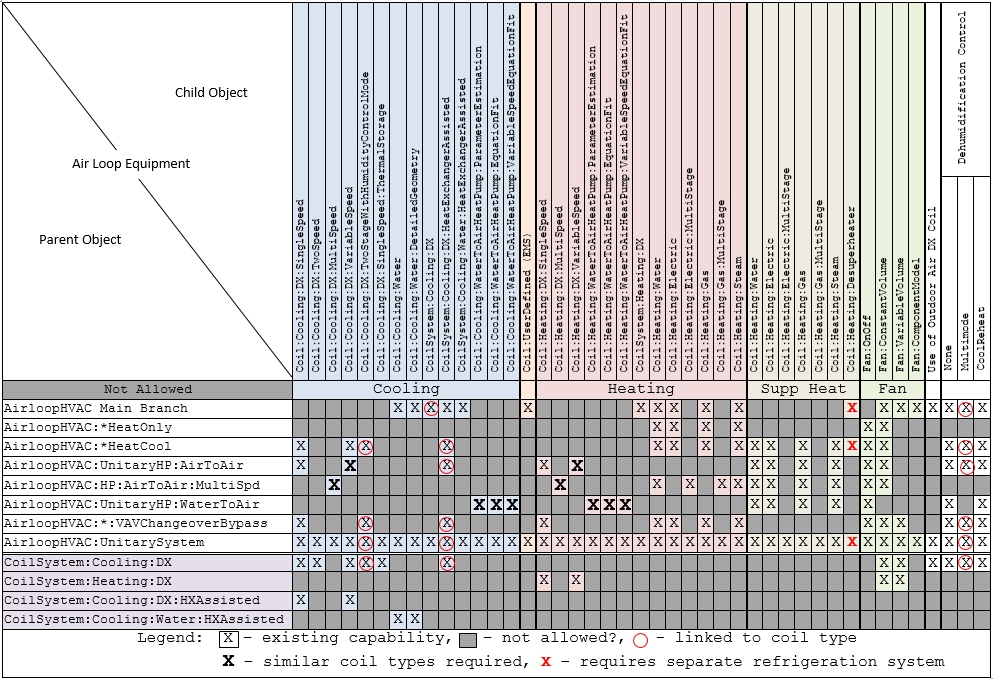
\includegraphics{media/AirLoopComponentMatrix.png}
\caption{}
\end{figure}

\subsection{AirLoopHVAC:UnitarySystem}\label{airloophvacunitarysystem}

The AirloopHVAC:UnitarySystem object is intended to replace all other air loop equipment, although other system types are still available. This system is unique in that it can accommodate all fan and coil types whereas other system types are specific to the type of fan and coil available for simulation. Additionally, although the AirloopHVAC:UnitarySystem is intended for use in the primary airloop, this object can be modeled as zone equipment (i.e., listed in a \hyperref[zonehvacequipmentlist]{ZoneHVAC:EquipmentList}) or as an outside air system component (i.e., listed in a \hyperref[airloophvacoutdoorairsystemequipmentlist]{AirLoopHVAC:OutdoorAirSystem:EquipmentList}). Water coil controllers are not required when these coil types are used with the AirloopHVAC:UnitarySystem object (i.e., leave the controller list name blank in the \hyperref[airloophvac]{AirLoopHVAC} object if water coils are used exclusively within the Unitary System).

The AirLoopHVAC:UnitarySystem object is a ``virtual'' component that consists of a fan component (OnOff, ConstantVolume, VariableVolume, or ComponentModel), a cooling coil component, a heating coil component, and a reheat coil as shown in Figure~\ref{fig:schematic-of-the-energyplus-unitary-system}. When a draw through configuration is desired, the fan is placed directly after the heating coil. If dehumidification control is selected, a reheat coil component is also required. If the reheat coil is present and the dehumidification control type input is not specified as CoolReheat, the reheat coil will not be active. All of the fan and coil components are optional which allows the AirLoopHVAC:UnitarySystem object to be configured for fan-only, heating-only, cooling-only, or both heating and cooling. It may also be applied without a fan, controlling one or more coils, similar to the function of \hyperref[coilsystemcoolingdx]{CoilSystem:Cooling:DX}.

\begin{figure}[hbtp] % fig 1
\centering
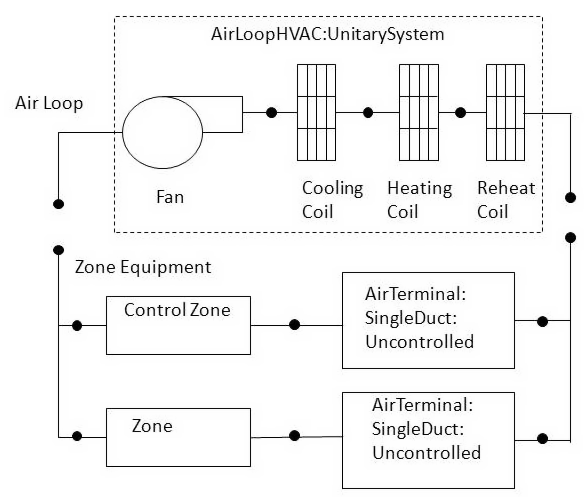
\includegraphics[width=0.9\textwidth, height=0.9\textheight, keepaspectratio=true]{media/image294.png}
\caption{Schematic of the EnergyPlus Unitary System \protect \label{fig:schematic-of-the-energyplus-unitary-system}}
\end{figure}

Links to the fan, cooling coil, heating coil and reheat coil specifications are provided in the unitary system input data syntax. In addition, the control zone name and the system design operating conditions are specified by the unitary system inputs.

\paragraph{Schedules And Availability Manager}

For unitary systems, don't use the night cycle manager. Use a scheduled availability manager and let the system be always on. Then use the Supply Air Fan Operating Mode Schedule Name in the unitary system to switch between continuous fan (for ventilation) during occupied periods and switch to cycling fan for unoccupied. The system will cycle on as the thermostat requests, and this way it will run just enough to meet the load - no need for a minimum cycle time.

Multi-speed fan chilled and hot water coils Air Handling Unit (AHU) can be modeled using Airloop Unitary System HVAC object (AirloopHVAC:UnitarySystem). AHU with chilled and hot water coils is setup by specifying \hyperref[fanonoff]{Fan:OnOff} and DesignSpecificationPerformance:MultiSpeed objects in Unitary System. The design specification performance object allows running the chilled and hot water coils capacity control using a multi-speed supply air fan. The multi-speed fan capacity control for chilled and hot water coil AHU is performed by modulating the supply air flow rate while maintaining a constant water flow rate. The chilled or hot water flow rates is set at maximum fixed flow rate when there is cooling or heating load and the water flow rate is set to zero when there is no load. Such control strategy is called two-position cooling or heating coil control. The fan speed selection depends on the current load, at lower load the fan is operated at minimum speed (Speed = 1) and the fan speed level increases progressively as the load increases until it reaches the maximum speed level specified. The multi-speed fan operation is modulated between the speeds to meet the current load. When the supply air fan is cycling between consecutive speeds levels, the speed ratio is calculated that indicates what fraction of the time step that the system run at the higher of the two speeds. At lower load, the fan may cycle on-off or run continuously depending the fan operating schedule specified. When the fan is cycling a part-load ratio is calculated to reflect the proportion of the system timestep the fan and coils were operating. In continuous fan operating mode only the coil cycles on-off and the part-load ratio applies to the coil only. Multi-speed fan capacity control is allowed with load based control type only.

\subsubsection{Inputs}\label{inputs-049}

\paragraph{Field: Name}\label{field-name-048}

This alpha field contains the identifying name for the unitary system.

\paragraph{Field: Control Type}\label{field-control-type-004}

This alpha field contains control type i.e.~load based or setpoint based for the unitary system. Valid choices are \textbf{Load}, \textbf{SetPoint} and \textbf{SingleZoneVAV}. Load and SingleZoneVAV control requires a Controlling Zone name. SetPoint control requires set points at each coil outlet node. A single set point at the outlet of the system is allowed but not recommended. If setpoint control is used and the system represents a heat pump (i.e., cooling and heating coils are both DX coils) then only one of these coils may operate at a time. SingleZoneVAV requires two distinct fan flow rates, namely the Cooling and Heating Supply Air Flow Rate and a lower No Load Supply Air Flow Rate which is used during times of reduced cooling or heating loads. SingleZoneVAV allows load control at low speed fan until the load exceeds available capacity or the outlet air temperature exceeds the specified limits where the fan speed is then increased. For the SingleZoneVAV control type, temperature limits are identified in the input fields for Minimum and Maximum Supply Air Temperature. Additionally, specific coil types are required for the SingleZoneVAV control type. The cooling coil types are \hyperref[coilcoolingwater]{Coil:Cooling:Water}, \hyperref[coilcoolingwaterdetailedgeometry]{Coil:Cooling:Water:DetailedGeometry} and \hyperref[coilcoolingdxsinglespeed]{Coil:Cooling:DX:SingleSpeed} while the heating coil types are \hyperref[coilheatingwater]{Coil:Heating:Water}, \hyperref[coilheatinggas-000]{Coil:Heating:Fuel}, \hyperref[coilheatingelectric]{Coil:Heating:Electric} and \hyperref[coilheatingdxsinglespeed]{Coil:Heating:DX:SingleSpeed}. If alternate coil types are used they are modeled using the load based control method.

\paragraph{Field: Controlling Zone or Thermostat Location}\label{field-controlling-zone-or-thermostat-location}

This alpha field contains the identifying zone name where the thermostat controlling the unitary system is located. This field is required when Load or SingleZoneVAV control type is selected.

\paragraph{Field: Dehumidification Control Type}\label{field-dehumidification-control-type-001}

This alpha field contains the type of dehumidification control. The following options are valid for this field:

\textbf{None} - meet sensible load only, no active dehumidification control. None is required when Control Type = SingleZoneVAV.

\textbf{Multimode} - activate enhanced dehumidification mode as needed and meet sensible load. This option is used to model DX equipment with a controllable heat exchanger assisting the DX cooling coil for improved dehumidification. It is valid only with cooling coil type = \hyperref[coilsystemcoolingdxheatexchangerassisted]{CoilSystem:Cooling:DX:HeatExchangerAssisted}.

\textbf{CoolReheat} - cool beyond the dry-bulb temperature set point as required to meet the high humidity setpoint. If cooling coil type = \hyperref[coilsystemcoolingdxheatexchangerassisted]{CoilSystem:Cooling:DX:HeatExchangerAssisted}, then the heat exchanger is assumed to always transfer energy between the cooling coil's inlet and outlet airstreams when the cooling coil is operating.

The default is \textbf{None}. For the other dehumidification control modes, the maximum humidity setpoint is used. This must be set using a \textbf{\hyperref[zonecontrolhumidistat]{ZoneControl:Humidistat}} object. When extra dehumidification is required, the system may not be able to meet the humidity setpoint if its full capacity is not adequate. If the dehumidification control type is specified as \textbf{CoolReheat}, then two additional inputs (reheat coil type and name) are also required as shown below. Although the reheat coil is required only when \textbf{CoolReheat} is selected, the optional reheat coil may be present for any of the allowed Dehumidification Control Types. If the reheat coil is present and the dehumidification control type is not specified as \textbf{CoolReheat}, the reheat coil will not be active,

\paragraph{Field: Availability Schedule Name}\label{field-availability-schedule-name-017}

This alpha field contains the schedule name which contains information on the availability of the unitary system to operate. A schedule value equal to 0 denotes that the unitary system must be off for that time period. A value greater than 0 denotes that the unitary system is available to operate during that time period. This schedule may be used to completely disable the unitary system as required. If this field is left blank, the schedule has a value of 1 for all time periods.

\paragraph{Field: Unitary System Air Inlet Node Name}\label{field-unitary-system-air-inlet-node-name}

This alpha field contains the unitary system air inlet node name.

\paragraph{Field: Unitary System Air Outlet Node Name}\label{field-unitary-system-air-outlet-node-name}

This alpha field contains the unitary system air outlet node name.

\paragraph{Field: Supply Fan Object Type}\label{field-supply-fan-object-type-000}

This alpha field contains the identifying type of supply air fan specified for the unitary system. Fan type must be \textbf{\hyperref[fanonoff]{Fan:OnOff},} \textbf{\hyperref[fanconstantvolume]{Fan:ConstantVolume}, \hyperref[fanvariablevolume]{Fan:VariableVolume}, or \hyperref[fancomponentmodel]{Fan:ComponentModel}}. \hyperref[fanconstantvolume]{Fan:ConstantVolume} is used when the Supply Air Fan Operating Mode Schedule values are never 0 and the fan operates continuously. \hyperref[fanonoff]{Fan:OnOff} is used when the fan cycles on and off with the cooling or heating coil (i.e.~Supply Air Fan Operating Mode Schedule values are at times 0). \hyperref[fanvariablevolume]{Fan:VariableVolume} is used for variable air volume systems or multi- or variable-speed coils. The \hyperref[fancomponentmodel]{Fan:ComponentModel} may be used in place of the ConstantVolume or VariableVolume fan types to more accurately represent fan performance.

\paragraph{Field: Supply Fan Name}\label{field-supply-fan-name}

This alpha field contains the unique identifying name given to the unitary system fan.

\paragraph{Field: Fan Placement}\label{field-fan-placement}

This alpha field has two choices: \textbf{BlowThrough} or \textbf{DrawThrough}. The first choice stands for ``blow through fan''. This means that the unit consists of a fan followed by the main cooling and heating coils and supplemental heating coil. The fan ``blows through'' the cooling and heating coils. The second choice stands for ``draw through fan''. This means that the unit consists of the main cooling/heating coil(s) followed by a fan, with the supplemental heater located at the outlet of the fan. The fan ``draws air through'' the cooling/heating coil(s). If this field is left blank, the default is blow through.

\paragraph{Field: Supply Air Fan Operating Mode Schedule Name}\label{supply-air-fan-operating-mode-schedule-name}

This alpha field specifies the name of the supply air fan operating mode schedule. The supply air fan operating mode may vary during the simulation based on time-of-day or with a change of season. Schedule values of 0 denote that the unitary system supply air fan and the heating or cooling coil cycle on and off together to meet the heating or cooling load (a.k.a. AUTO fan). Schedule values other than 0 denote that the supply fan runs continuously while the heating or cooling coil cycles to meet the load. The SingleZoneVAV control type is only active when the supply air fan runs continuously (i.e., during cycling fan operation the Control Type = Load model is used).

\paragraph{Field: Heating Coil Object Type}\label{field-heating-coil-object-type-002}

This alpha field contains the identifying type of heating coil specified in the unitary system. The hot water and steam heating coils require specifying plant loop, branches, and connector objects to support the heating coils, and are placed on the demand side of the plantloop. Only specific coil types are allowed when Control Type = SingleZoneVAV as noted. Allowable coil types are:

\begin{itemize}
\item
  \hyperref[coilheatingdxsinglespeed]{Coil:Heating:DX:SingleSpeed}
\item
  Coil:Heating:DX:TwoSpeed
\item
  \hyperref[coilheatingdxmultispeed]{Coil:Heating:DX:MultiSpeed}
\item
  \hyperref[coilheatingdxvariablespeed]{Coil:Heating:DX:VariableSpeed}
\item
  \hyperref[coilheatingwatertoairheatpumpparameterestimation]{Coil:Heating:WaterToAirHeatPump:ParameterEstimation}
\item
  \hyperref[coilheatingwatertoairheatpumpequationfit]{Coil:Heating:WaterToAirHeatPump:EquationFit}
\item
  \hyperref[coilheatingwatertoairheatpumpvariablespeedequationfit]{Coil:Heating:WaterToAirHeat\hyperref[pumpvariablespeed]{Pump:VariableSpeed}EquationFit}
\item
  \hyperref[coilheatinggas-000]{Coil:Heating:Fuel}
\item
  \hyperref[coilheatinggasmultistage]{Coil:Heating:Gas:MultiStage}
\item
  \hyperref[coilheatingelectric]{Coil:Heating:Electric}
\item
  \hyperref[coilheatingelectricmultistage]{Coil:Heating:Electric:MultiStage}
\item
  \hyperref[coilheatingwater]{Coil:Heating:Water}
\item
  \hyperref[coilheatingsteam]{Coil:Heating:Steam}
\item
  \hyperref[coilheatingdesuperheater]{Coil:Heating:Desuperheater}
\item
  \hyperref[coiluserdefined]{Coil:UserDefined}
\end{itemize}

\paragraph{Field: Heating Coil Name}\label{field-heating-coil-name-002}

This alpha field contains the identifying name given to the unitary system heating coil.

\paragraph{Field: DX Heating Coil Sizing Ratio}\label{field-dx-heating-coil-sizing-ratio}

This numeric field is used to adjust heat pump heating capacity with respect to DX cooling capacity. It is used only for DX heat pump configurations (i.e., a DX cooling and heating coil is used).

\paragraph{Field: Cooling Coil Object Type}\label{field-cooling-coil-object-type-002}

This alpha field contains the identifying type of cooling coil specified in the unitary system. Allowable coil types are:

\begin{itemize}
\item
  \hyperref[coilcoolingdxsinglespeed]{Coil:Cooling:DX:SingleSpeed}
\item
  \hyperref[coilcoolingdxsinglespeedthermalstorage]{Coil:Cooling:DX:SingleSpeed:ThermalStorage}
\item
  \hyperref[coilcoolingdxtwospeed]{Coil:Cooling:DX:TwoSpeed}
\item
  \hyperref[coilcoolingdxmultispeed]{Coil:Cooling:DX:MultiSpeed}
\item
  \hyperref[coilcoolingdxvariablespeed]{Coil:Cooling:DX:VariableSpeed}
\item
  \hyperref[coilcoolingdxtwostagewithhumiditycontrolmode]{Coil:Cooling:DX:TwoStageWithHumidityControlMode}
\item
  \hyperref[coilsystemcoolingdxheatexchangerassisted]{CoilSystem:Cooling:DX:HeatExchangerAssisted}
\item
  \hyperref[coilcoolingwatertoairheatpumpparameterestimation]{Coil:Cooling:WaterToAirHeatPump:ParameterEstimation}
\item
  \hyperref[coilcoolingwatertoairheatpumpequationfit]{Coil:Cooling:WaterToAirHeatPump:EquationFit}
\item
  \hyperref[coilcoolingwatertoairheatpumpvariablespeedequationfit]{Coil:Cooling:WaterToAirHeat\hyperref[pumpvariablespeed]{Pump:VariableSpeed}EquationFit}
\item
  \hyperref[coilcoolingwater]{Coil:Cooling:Water}
\item
  \hyperref[coilcoolingwaterdetailedgeometry]{Coil:Cooling:Water:DetailedGeometry}
\item
  \hyperref[coilsystemcoolingwaterheatexchangerassisted]{CoilSystem:Cooling:Water:HeatExchangerAssisted}
\item
  \hyperref[coiluserdefined]{Coil:UserDefined}
\end{itemize}

\paragraph{Field: Cooling Coil Name}\label{field-cooling-coil-name-002}

This alpha field contains the identifying name given to the unitary system cooling coil.

\paragraph{Field: Use DOAS DX Cooling Coil}\label{field-use-doas-dx-cooling-coil}

This input field enables DX Cooling coils to be used for 100\% outdoor air dedicated outdoor air system applications. There are two choices Yes or No. If Yes, the DX coil is used as 100\% outdoor DX coil. If No, the DX coil is used as regular DX coil. This input field is optional and the default is No. No should be specified when selecting the SingleZoneVAV control type.

\paragraph{Field: Minimum Supply Air Temperature}

When Use DOAS DX Cooling Coil is specified as Yes, this input field is the DX Cooling coils leaving minimum air temperature for frost control. The DX cooling coil leaving air temperature is not allowed to exceed this minimum air temperature. The DX cooling coil frost controller adjusts or limits the desired coil outlet air setpoint temperature when the coil outlet temperature exceeds this minimum temperature limit specified. The minimum and maximum values of this input field are 0.0\(^{o}\)C and 7.5\(^{o}\)C, and the default value is 2.0\(^{o}\)C. This field is not autosizable when the input for Use DOAS DX Cooling Coil = Yes. When Control Type = SingleZoneVAV, enter the minimum air temperature limit for reduced fan speed in cooling mode. For SingleZoneVAV, the maximum limit for the minimum supply air temperature is 20.0\(^{o}\)C. Additionally, for the SingleZoneVAV model this input does not limit the minimum supply air temperature resulting from cooling coil operation at high fan speed.


\paragraph{Field: Latent Load Control}\label{field-latent-load-control}

This alpha field defines the latent load control method. Available choices are SensibleOnlyLoadControl, LatentOnlyLoadControl, LatentWithSensibleLoadControl, or LatentOrSensibleLoadControl. The default choice is SensibleOnlyLoadControl. The SensibleOnlyLoadControl choice will operate to meet only a sensible load and is also required when SingleZoneVAV control is selected. The LatentOnlyLoadConrol will operate to meet only a latent load. The LatentWithSensibleLoadControl will operate to meet the latent load only if there is a sensible load. The LatentOrSensibleLoadControl will operate to meet either a latent or sensible load.

\paragraph{Field: Supplemental Heating Coil Object Type}\label{field-supplemental-heating-coil-object-type}

This alpha field contains the identifying type of supplemental heating coil specified in the unitary system. The hot water and steam heating coils require specifying plant loop, branches, and connector objects to support the heating coils, and are placed on the demand side of the plant loop. The \hyperref[coiluserdefined]{Coil:UserDefined} object must be configured as a heating coil. Supplemental heating type must be one of:

\begin{itemize}
\item
  \hyperref[coilheatingelectric]{Coil:Heating:Electric}
\item
  \hyperref[coilheatinggas-000]{Coil:Heating:Fuel}
\item
  \hyperref[coilheatingdesuperheater]{Coil:Heating:Desuperheater}
\item
  \hyperref[coilheatingwater]{Coil:Heating:Water}
\item
  \hyperref[coilheatingsteam]{Coil:Heating:Steam}
\item
  \hyperref[coiluserdefined]{Coil:UserDefined}
\end{itemize}

\paragraph{Field: Supplemental Heating Coil Name}\label{field-supplemental-heating-coil-name}

This alpha field contains the identifying name given to the unitary system supplemental or reheat coil object. This coil provides supplemental heat during heating mode operation, or reheats the supply air during dehumidification mode operation. For set point based control, all coils will control to their respective outlet air temperature set point.

\paragraph{Field: Cooling Supply Air Flow Rate Method}\label{field-cooling-supply-air-flow-rate-method-000}

This alpha field defines the supply air flow method during cooling operation. Available choices are SupplyAirFlowRate, FlowPerFloorArea, FractionOfAutosizedCoolingValue, FlowPerCoolingCapacity. For each of the choices, a corresponding air flow rate for cooling must be specified. If the system does not have a cooling coil a 0 may be entered for cooling air flow rate and/or no load supply air flow rate to turn the fan off when cooling is not required.

\paragraph{Field: Cooling Supply Air Flow Rate}\label{field-cooling-supply-air-flow-rate-001}

This numeric field defines the supply air flow rate leaving the unitary system in cubic meters per second when the cooling coil is operating. Values must be greater than 0 if the cooling coil is present or this field is autosizable. Required field when Cooling Supply Air Flow Rate Method is \textbf{SupplyAirFlowRate}.

\paragraph{Field: Cooling Supply Air Flow Rate Per Floor Area}\label{field-cooling-supply-air-flow-rate-per-floor-area}

This numeric field defines the supply air flow rate per floor area leaving the unitary system in meters per second when the cooling coil is operating. Values must be greater than 0 if the cooling coil is present or this field is autosizable. Required field when Cooling Supply Air Flow Rate Method is \textbf{FlowPerFloorArea}.

\paragraph{Field: Cooling Fraction of Autosized Design Cooling Supply Air Flow Rate}\label{field-cooling-fraction-of-autosized-design-cooling-supply-air-flow-rate}

This numeric field defines the fraction of autosized supply air flow rate leaving the unitary system when the cooling coil is operating. Values must be greater than 0 if the cooling coil is present or this field is autosizable. Required field when Cooling Supply Air Flow Rate Method is \textbf{FractionOfAutosizedCoolingValue}.

\paragraph{Field: Cooling Supply Air Flow Rate Per Unit of Capacity}\label{field-cooling-supply-air-flow-rate-per-unit-of-capacity}

This numeric field defines the supply air flow rate per unit of capacity leaving the unitary system when the cooling coil is operating. Values must be greater than 0 if the cooling coil is present or this field is autosizable. Required field when Cooling Supply Air Flow Rate Method is \textbf{FlowPerCoolingCapacity}.

\paragraph{Field: Heating Supply Air Flow Rate Method}\label{field-heating-supply-air-flow-rate-method-000}

This alpha field defines the supply air flow method during heating operation. Available choices are SupplyAirFlowRate, FlowPerFloorArea, FractionOfAutosizedHeatingValue, FlowPerHeatingCapacity. For each of the choices, a corresponding air flow rate for heating must be specified. If the system does not have a heating coil a 0 may be entered for heating air flow rate and/or no load supply air flow rate to turn the fan off when heating is not required.

\paragraph{Field: Heating Supply Air Flow Rate}\label{field-heating-supply-air-flow-rate-001}

This numeric field defines the supply air flow rate leaving the unitary system in cubic meters per second when the heating coil is operating. Values must be greater than 0 if the heating coil is present or this field is autosizable. Required field when Heating Supply Air Flow Rate Method is \textbf{SupplyAirFlowRate}.

\paragraph{Field: Heating Supply Air Flow Rate Per Floor Area}\label{field-heating-supply-air-flow-rate-per-floor-area}

This numeric field defines the supply air flow rate per floor area leaving the unitary system in meters per second when the heating coil is operating. Values must be greater than 0 if the heating coil is present or this field is autosizable. Required field when Heating Supply Air Flow Rate Method is \textbf{FlowPerFloorArea}.

\paragraph{Field: Heating Fraction of Autosized Design Heating Supply Air Flow Rate}\label{field-heating-fraction-of-autosized-design-heating-supply-air-flow-rate}

This numeric field defines the fraction of autosized supply air flow rate leaving the unitary system when the heating coil is operating. Values must be greater than 0 if the heating coil is present or this field is autosizable. Required field when Heating Supply Air Flow Rate Method is \textbf{FractionOfAutosizedHeatingValue}.

\paragraph{Field: Heating Supply Air Flow Rate Per Unit of Capacity}\label{field-heating-supply-air-flow-rate-per-unit-of-capacity}

This numeric field defines the supply air flow rate per unit of capacity leaving the unitary system when the heating coil is operating. Values must be greater than 0 if the heating coil is present or this field is autosizable. Required field when Heating Supply Air Flow Rate Method is \textbf{FlowPerHeatingCapacity}.

\paragraph{Field: No Load Supply Air Flow Rate Method}\label{field-no-load-supply-air-flow-rate-method}

This alpha field defines the supply air flow method when neither cooling or heating is required. Available choices are SupplyAirFlowRate, FlowPerFloorArea, FractionOfAutosizedCoolingValue, FractionOfAutosizedHeatingValue, FlowPerCoolingCapacity, FlowPerHeatingCapacity. For each of the choices, a corresponding air flow rate must be specified. The following fields are also used to specify the lower air flow rate for the SingleZoneVAV control method with recommendations of greater than or equal to 67\% of the Cooling or Heating Supply Air Flow Rate when any DX coil is used and 50\% for other coil types.

\paragraph{Field: No Load Supply Air Flow Rate}\label{field-no-load-supply-air-flow-rate-000}

This numeric field defines the supply air flow rate leaving the unitary system in cubic meters per second when neither cooling or heating is required (i.e., main cooling/heating coils and supplemental heater are off but the supply air fan operates). This field is only used when the unitary system operating mode is specified as continuous fan operation. Values must be greater than or equal to 0, or this field is autosizable. If this field is autosized, then it is sized to the minimum of the heating and cooling lowest speed supply air flow rate. If the unitary system operating mode is specified as continuous fan operation and this value is set to zero or this field is left blank, then the model assumes that the supply air flow rate when no cooling/heating is needed is equal to the supply air flow rate when the compressor was last operating (for cooling operation or heating operation).

\paragraph{Field: No Load Supply Air Flow Rate Per Floor Area}\label{field-no-load-supply-air-flow-rate-per-floor-area}

This numeric field defines the supply air flow rate per floor area leaving the unitary system in meters per second when neither cooling or heating coil is operating. Values must be greater than or equal to 0 or this field is autosizable. Required field when No Load Supply Air Flow Rate Method During is \textbf{FlowPerFloorArea}.

\paragraph{Field: No Load Fraction of Autosized Cooling Supply Air Flow Rate}\label{field-no-load-fraction-of-autosized-cooling-supply-air-flow-rate}

This numeric field defines the fraction of autosized supply air flow rate leaving the unitary system when neither cooling or heating coil is operating. Values must be greater than or equal to 0 or this field is autosizable. Required field when No Load Supply Air Flow Rate Method is \textbf{FractionOfAutosizedCoolingValue}.

\paragraph{Field: No Load Fraction of Autosized Heating Supply Air Flow Rate}\label{field-no-load-fraction-of-autosized-heating-supply-air-flow-rate}

This numeric field defines the fraction of autosized supply air flow rate leaving the unitary system when the neither cooling or heating coil is operating. Values must be greater than or equal to 0 or this field is autosizable. Required field when No Load Supply Air Flow Rate Method is \textbf{FractionOfAutosizedHeatingValue}.

\paragraph{Field: No Load Supply Air Flow Rate Per Unit of Capacity During Cooling Operation}\label{field-no-load-supply-air-flow-rate-per-unit-of-capacity-during-cooling-operation}

This numeric field defines the supply air flow rate per unit of capacity leaving the unitary system when neither cooling or heating is operating. Values must be greater than or equal to 0 or this field is autosizable. Required field when No Load Supply Air Flow Rate Method is \textbf{FlowPerCoolingCapacity}.

\paragraph{Field: No Load Supply Air Flow Rate Per Unit of Capacity During Heating Operation}\label{field-no-load-supply-air-flow-rate-per-unit-of-capacity-during-heating-operation}

This numeric field defines the supply air flow rate per unit of capacity leaving the unitary system when neither cooling or heating is operating. Values must be greater than or equal to 0 or this field is autosizable. Required field when No Load Supply Air Flow Rate Method is \textbf{FlowPerHeatingCapacity}.

\paragraph{Field: Maximum Supply Air Temperature}\label{field-maximum-supply-air-temperature-000}

This numeric field contains the design operating air outlet temperature in degrees C when the unitary system is heating. If this input field is left blank, the default value is 80 C. When Control Type = SingleZoneVAV, enter the maximum air temperature limit for reduced fan speed in heating model. For the SingleZoneVAV model this input does not limit the maximum supply air temperature resulting from heating or supplemental heating coil operation at high fan speed.  This field is autosizable.


\paragraph{Field: Maximum Outdoor Dry-Bulb Temperature for Supplemental Heater Operation}\label{field-maximum-outdoor-dry-bulb-temperature-for-supplemental-heater-operation}

This numeric field defines the outdoor air dry-bulb temperature above which the heat pump supplemental heating coil is disabled.~ The temperature for this input field must be less than or equal to 21 C. If this input field is left blank, the default value is 21 C.

\paragraph{Field: Outdoor Dry-Bulb Temperature Sensor Node Name}\label{field-outdoor-dry-bulb-temperature-sensor-node-name}

This alpha field specifies the name of the outdoor node which controls the operation of the supplemental heating coil. If this field is left blank, the outdoor temperature is based solely on the weather data. If this field is not blank, the node name specified must also be listed in an \hyperref[outdoorairnode]{OutdoorAir:Node} object where the height of the node is taken into consideration when calculating outdoor temperature from the weather data. Alternately, the node name must be specified in an \hyperref[outdoorairnodelist]{OutdoorAir:NodeList} object where the outdoor temperature is taken directly from the weather data.

\paragraph{Field: Maximum Cycling Rate}\label{field-maximum-cycling-rate-001}

This numeric field contains the maximum on-off cycling rate for the compressor, which occurs at 50\% run time fraction. Suggested values are shown in Figure~\ref{fig:suggested-values-for-maximum-cycling-rate}. (Henderson et al. 1999):

\begin{figure}[htbp]
\centering
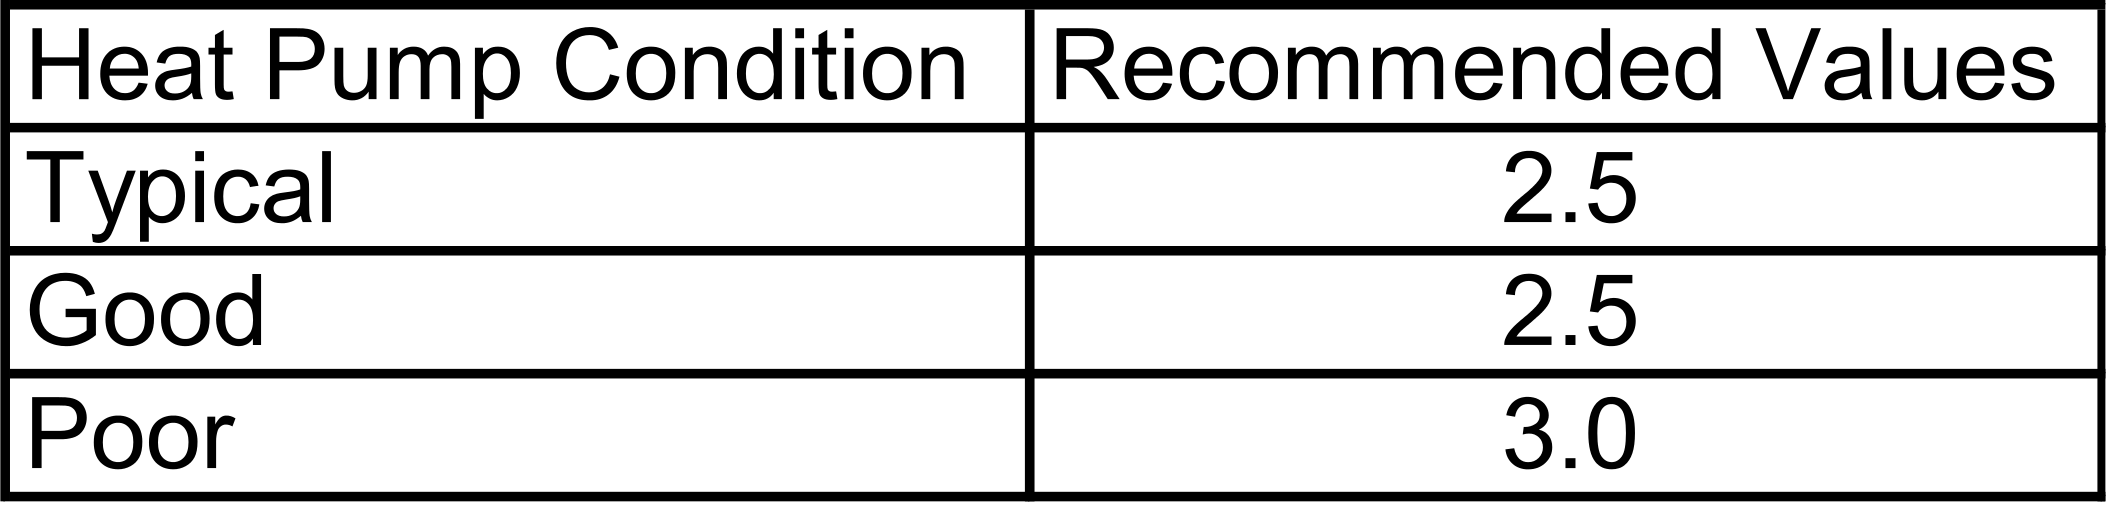
\includegraphics{media/image295.png}
\caption{Suggested values for maximum cycling rate \protect \label{fig:suggested-values-for-maximum-cycling-rate}}
\end{figure}

\paragraph{Field: Heat Pump Time Constant}\label{field-heat-pump-time-constant-000}

This numeric field contains the time constant for the cooling coil's capacity to reach steady state after startup. Suggested values are shown in Figure~\ref{fig:suggested-values-for-heat-pump-time-constant}. (Henderson et al. 1999):

\begin{figure}[htbp]
\centering
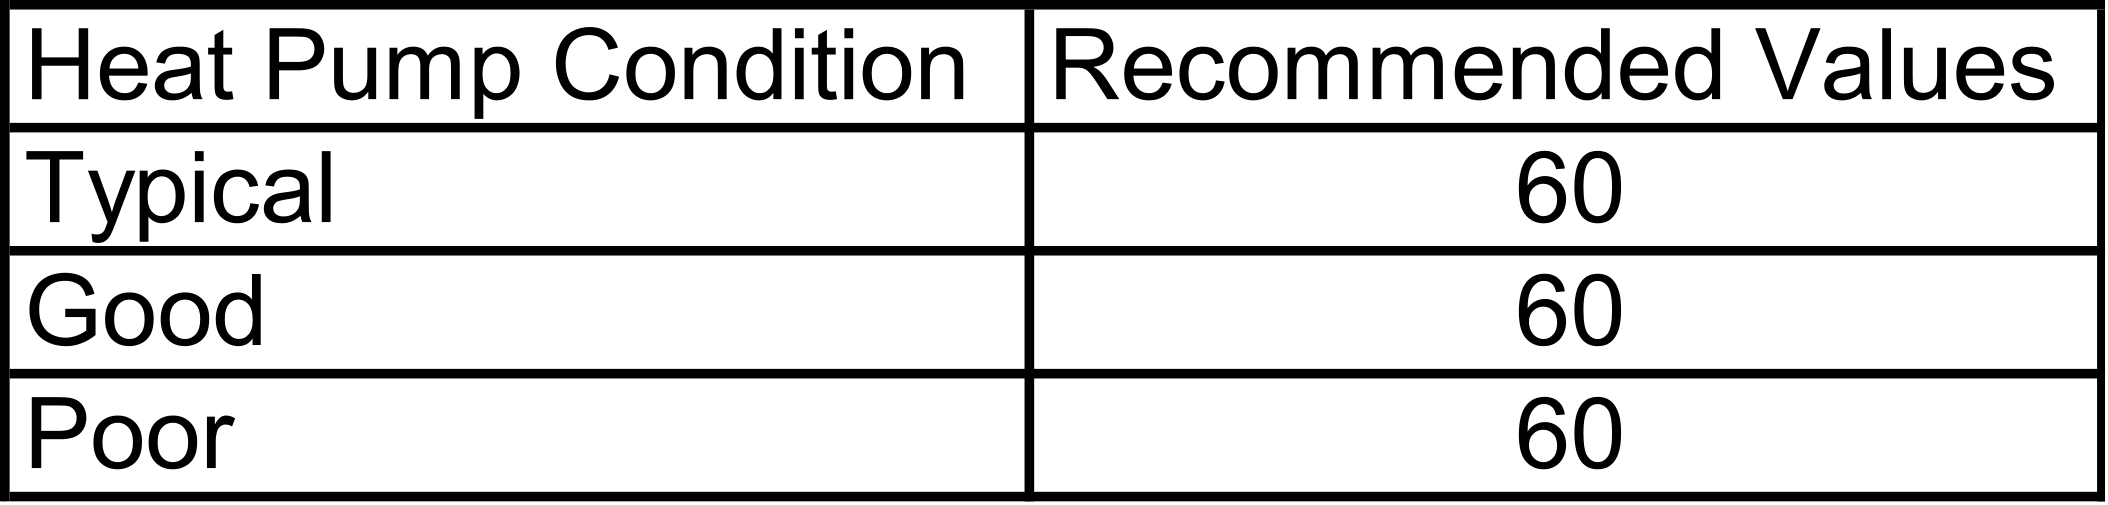
\includegraphics{media/image296.png}
\caption{Suggested values for heat pump time constant \protect \label{fig:suggested-values-for-heat-pump-time-constant}}
\end{figure}

\paragraph{Field: Fraction of On-Cycle Power Use}\label{field-fraction-of-on-cycle-power-use-000}

This numeric field contains the fraction of on-cycle power use to adjust the part load fraction based on the off-cycle power consumption due to crankcase heaters, controls, fans, and etc. Suggested value values are shown in Figure~\ref{fig:suggested-values-for-fraction-of-on-cycle-power-use}. (Henderson et al. 1999):

\begin{figure}[htbp]
\centering
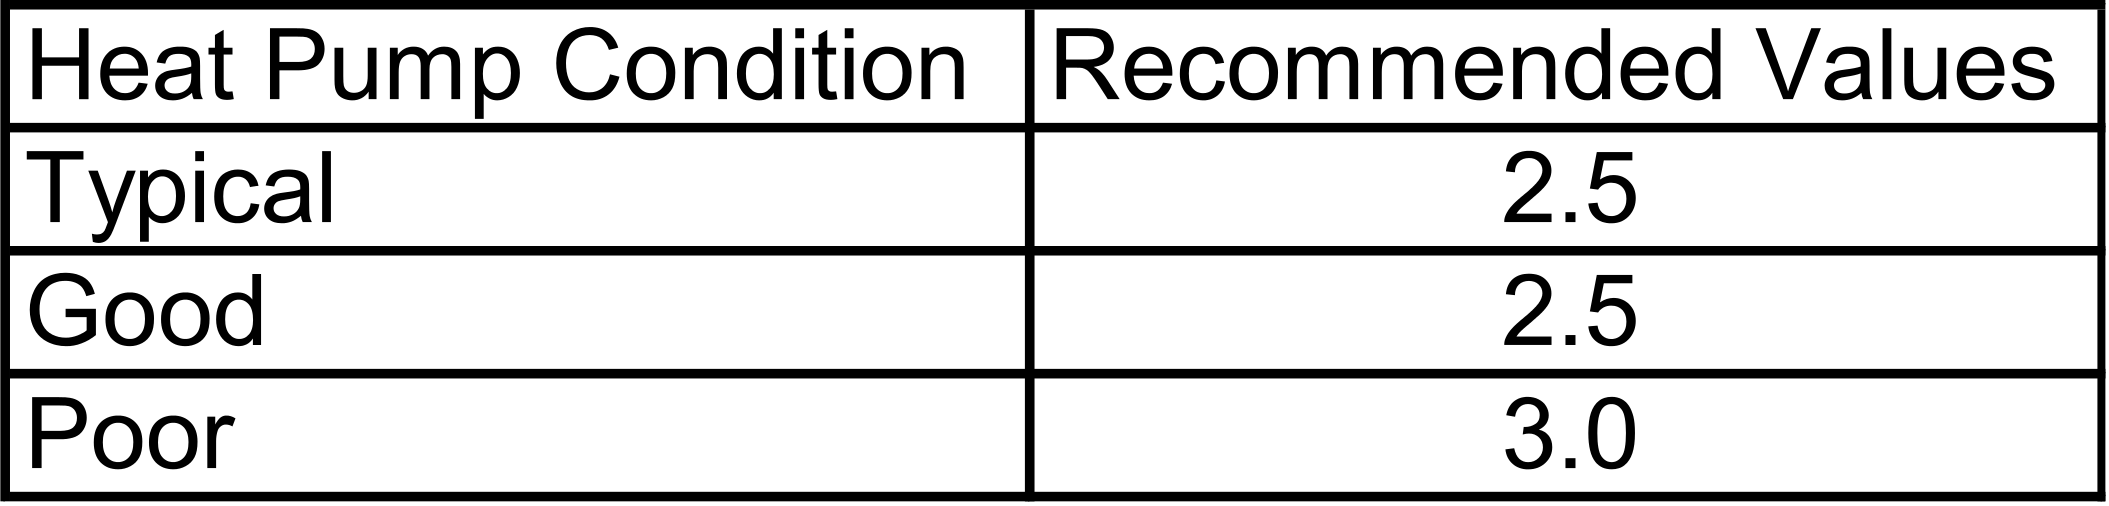
\includegraphics{media/image297.png}
\caption{Suggested values for fraction of on cycle power use \protect \label{fig:suggested-values-for-fraction-of-on-cycle-power-use}}
\end{figure}

\paragraph{Field: Heat Pump Fan Delay Time}\label{field-heat-pump-fan-delay-time-000}

This numeric field contains the time delay for the heat pump supply air fan to shut off after the compressor cycles off in seconds. This value can be obtained from the manufacturer or the heat pump catalog. Enter a value of zero when the heat pump's fan operating mode is continuous. Suggested value is 60 seconds.

\paragraph{Field: Ancillary On-Cycle Electric Power}\label{field-ancillary-on-cycle-electric-power}

This field defines ancillary electrical power (W) consumed during the on-cycle period (i.e., when the cooling or heating coil is operating). The model assumes that this ancillary power does not contribute to heating the supply air. The minimum value for this field is 0.0, and the default value is also 0.0 if the field is left blank.

\paragraph{Field: Ancillary Off-Cycle Electric Power}\label{field-ancillary-off-cycle-electric-power}

This field defines ancillary electrical power (W) consumed during the off-cycle period (i.e., when the cooling and heating coil are not operating). The model assumes that this ancillary power does not contribute to heating the supply air. The minimum value for this field is 0.0, and the default value is also 0.0 if the field is left blank.

\paragraph{Field: Design Heat Recovery Water Flow Rate}\label{field-design-heat-recovery-water-flow-rate-001}

This optional input field defines the design water flow rate used if the heat recovery option is being simulated. If this value is greater than 0.0 then a heat recovery loop must be specified and attached to the multispeed heat pump using the next 2 node fields. To determine how the heat recovery algorithm works, refer to the EnergyPlus Engineering Reference in the AirLoopHVAC:UnitarySystem with Heat Recovery section. The units for this input value are cubic meters per second.

\paragraph{Field: Maximum Temperature for Heat Recovery}\label{field-maximum-temperature-for-heat-recovery}

This field sets the maximum temperature (in degrees C) that this heat pump can produce for heat recovery. The idea behind this field is that the current models do not take temperatures into account for availability and they just pass Q's around the loop without a temperature limit. This temperature limit puts an upper bound on the recovered heat and limits the max temperature leaving the component.

As temperatures in the loop approach the maximum temperature, the temperature difference between the entering water and the surfaces in the piece of equipment becomes smaller. For the given heat recovery flow rate and that temperature difference the amount of heat recovered will be reduced, and eventually there will be no heat recovered when the entering water temperature is equal to the maximum temperature specified by the user in this field. The reduced amount of heat recovered will diminish if the temperature of the loop approach is the maximum temperature, and this will show up in the reporting. This allows the user to set the availability or the quality of the heat recovered for usage in other parts of the system or to heat domestic hot water supply.

\paragraph{Field: Heat Recovery Water Inlet Node Name}\label{field-heat-recovery-water-inlet-node-name-000}

This alpha field contains the identifying name for the heat recovery side inlet node.

\paragraph{Field: Heat Recovery Water Outlet Node Name}\label{field-heat-recovery-water-outlet-node-name-000}

This alpha field contains the identifying name for the heat recovery side outlet node.

\paragraph{Field: Design Specification Multispeed Object Type}\label{field-design-specification-multispeed-object-type}

This alpha field contains the identifying type for the design specification multispeed object. This field is only needed when multispeed cooling or heating coil is specified.

\paragraph{Field: Design Specification Multispeed Object Name}\label{field-design-specification-multispeed-object-name}

This alpha field contains the identifying name for the design specification multispeed object. This field is only needed when multispeed cooling or heating coil is specified.

As shown in the example below, correct specification of the heat/cool unitary system requires specification of the following objects in addition to the unitary system object:

\begin{enumerate}
\def\labelenumi{\arabic{enumi})}
\item
  Fan (\hyperref[fanonoff]{Fan:OnOff} or \hyperref[fanconstantvolume]{Fan:ConstantVolume})
\item
  Cooling coil
\item
  Heating coil
\item
  Reheat coil
\item
  Direct air unit (\hyperref[airterminalsingleductconstantvolumenoreheat]{AirTerminal:SingleDuct:ConstantVolume:NoReheat}) for each zone served by the unitary system when used in an air loop
\end{enumerate}

\begin{lstlisting}

AirLoopHVAC:UnitarySystem,
  DXAC Heat Pump 1,            !- Name
  Load,                        !- Control Type
  East Zone,                   !- Controlling Zone or Thermostat Location
  ,                            !- Dehumidification Control Type
  FanAndCoilAvailSched,        !- Availability Schedule Name
  Mixed Air Node,              !- Air Inlet Node Name
  Air Loop Outlet Node,        !- Air Outlet Node Name
  Fan:OnOff,                   !- Supply Fan Object Type
  Supply Fan 1,                !- Supply Fan Name
  BlowThrough,                 !- Fan Placement
  FanModeSchedule,             !- Supply Air Fan Operating Mode Schedule Name
  Coil:Heating:DX:MultiSpeed,  !- Heating Coil Object Type
  Heat Pump DX Heating Coil 1, !- Heating Coil Name
  ,                            !- DX Heating Coil Sizing Ratio
  Coil:Cooling:DX:MultiSpeed,  !- Cooling Coil Object Type
  Heat Pump ACDXCoil 1,        !- Cooling Coil Name
  ,                            !- Use DOAS DX Cooling Coil
  ,                            !- Minimum Supply Air Temperature {C}
  ,                            !- Latent Load Control
  Coil:Heating:Fuel,           !- Supplemental Heating Coil Object Type
  Supp Gas Heating Coil 1,     !- Supplemental Heating Coil Name
  SupplyAirFlowRate,           !- Cooling Supply Air Flow Rate Method
  1.7,                         !- Cooling Supply Air Flow Rate {m3/s}
  ,                            !- Cooling Supply Air Flow Rate Per Floor Area {m3/s-m2}
  ,                            !- Cooling Fraction of Autosized Cooling Supply Air Flow Rate
  ,                            !- Cooling Supply Air Flow Rate Per Unit of Capacity {m3/s-W}
  SupplyAirFlowRate,           !- Heating Supply Air Flow Rate Method
  1.7,                         !- Heating Supply Air Flow Rate {m3/s}
  ,                            !- Heating Supply Air Flow Rate Per Floor Area {m3/s-m2}
  ,                            !- Heating Fraction of Autosized Heating Supply Air Flow Rate
  ,                            !- Heating Supply Air Flow Rate Per Unit of Capacity {m3/s-W}
  SupplyAirFlowRate,           !- No Load Supply Air Flow Rate Method
  0.2,                         !- No Load Supply Air Flow Rate {m3/s}
  ,                            !- No Load Supply Air Flow Rate Per Floor Area {m3/s-m2}
  ,                            !- No Load Fraction of Autosized Cooling Supply Air Flow Rate
  ,                            !- No Load Fraction of Autosized Heating Supply Air Flow Rate
  ,                            !- No Load Supply Air Flow Rate Per Unit of Capacity during Cooling Operation {m3/s-W}
  ,                            !- No Load Supply Air Flow Rate Per Unit of Capacity during Heating Operation {m3/s-W}
  50,                          !- Maximum Supply Air Temperature {C}
  21,                          !- Maximum Outdoor Dry-Bulb Temperature for Supplemental Heater Operation {C}
  ,                            !- Outdoor Dry-Bulb Temperature Sensor Node Name
  ,                            !- Maximum Cycling Rate {cycles/hr}
  ,                            !- Heat Pump Time Constant {s}
  ,                            !- Fraction of On-Cycle Power Use
  ,                            !- Heat Pump Fan Delay Time {s}
  ,                            !- Ancillary On-Cycle Electric Power {W}
  ,                            !- Ancillary Off-Cycle Electric Power {W}
  ,                            !- Design Heat Recovery Water Flow Rate {m3/s}
  ,                            !- Maximum Temperature for Heat Recovery {C}
  ,                            !- Heat Recovery Water Inlet Node Name
  ,                            !- Heat Recovery Water Outlet Node Name
  UnitarySystemPerformance:Multispeed,  !- Design Specification Multispeed Object Type
  MyMultispeedHPSpec;          !- Design Specification Multispeed Object Name

  UnitarySystemPerformance:Multispeed,
  MyMultispeedHPSpec,          !- Name
  4,                           !- Number of Speeds for Heating
  4,                           !- Number of Speeds for Cooling
  No,                          !- Single Mode Operation
  ,                            !- No Load Supply Air Flow Rate Ratio
  0.235294118,                 !- Heating Speed 1 Supply Air Flow Ratio
  0.235294118,                 !- Cooling Speed 1 Supply Air Flow Ratio
  0.470588235,                 !- Heating Speed 2 Supply Air Flow Ratio
  0.470588235,                 !- Cooling Speed 2 Supply Air Flow Ratio
  0.705882353,                 !- Heating Speed 3 Supply Air Flow Ratio
  0.705882353,                 !- Cooling Speed 3 Supply Air Flow Ratio
  1.0,                         !- Heating Speed 4 Supply Air Flow Ratio
  1.0;                         !- Cooling Speed 4 Supply Air Flow Ratio
\end{lstlisting}

\subsubsection{Outputs}\label{outputs-038}

\begin{itemize}
\item
  HVAC,Average, Unitary System Fan Part Load Ratio {[]}
\item
  HVAC,Average, Unitary System Compressor Part Load Ratio
\item
  HVAC,Average,Unitary System Total Cooling Rate {[}W{]}
\item
  HVAC,Average,Unitary System Total Heating Rate {[}W{]}
\item
  HVAC,Average,Unitary System Sensible Cooling Rate {[}W{]}
\item
  HVAC,Average,Unitary System Sensible Heating Rate {[}W{]}
\item
  HVAC,Average,Unitary System Latent Cooling Rate {[}W{]}
\item
  HVAC,Average,Unitary System Latent Heating Rate {[}W{]}
\item
  HVAC,Average,Unitary System Ancillary Electric Power{[}W{]}
\end{itemize}

Load based and SingleZoneVAV control outputs
\begin{itemize}
\tightlist
\item
HVAC,Average,Unitary System Predicted Sensible Load to Setpoint Heat Transfer Rate [W]
\item
HVAC,Average,Unitary System Predicted Moisture Load to Setpoint Heat Transfer Rate [W]
\end{itemize}

Two speed coil outputs

\begin{itemize}
\tightlist
\item
  HVAC,Average,Unitary System Cycling Ratio {[]}
\item
  HVAC,Average,Unitary System Compressor Speed Ratio {[]}
\end{itemize}

Multi speed coil outputs

\begin{itemize}
\item
  HVAC,Average,Unitary System DX Coil Cycling Ratio {[]}
\item
  HVAC,Average,Unitary System DX Coil Speed Ratio {[]}
\item
  HVAC,Average,Unitary System DX Coil Speed Level {[]}
\item
  HVAC,Average,Unitary System Electric Power{[}W{]}
\item
  HVAC,Sum,Unitary System Electric Energy {[}J{]}
\item
  HVAC,Sum,Unitary System Cooling Ancillary Electric Energy {[}J{]}
\item
  HVAC,Sum,Unitary System Heating Ancillary Electric Energy {[}J{]}
\end{itemize}

Multi speed coil outputs(If heat recovery is specified)

\begin{itemize}
\item
  HVAC,Average, Unitary System Heat Recovery Rate {[}W{]}
\item
  HVAC,Average, Unitary System Heat Recovery Inlet Temperature {[}C{]}
\item
  HVAC,Average, Unitary System Heat Recovery Outlet Temperature {[}C{]}
\item
  HVAC,Average, Unitary System Heat Recovery Fluid Mass Flow Rate {[}kg/s{]}
\item
  HVAC,Sum, Unitary System Heat Recovery Energy {[}J{]}
\end{itemize}

Variable speed coils

\begin{itemize}
\item
  HVAC,Average, Unitary System Requested Sensible Cooling Rate {[}W{]}
\item
  HVAC,Average, Unitary System Requested Latent Cooling Rate {[}W{]}
\end{itemize}


Water to air heat pump outputs

\begin{itemize}
\item
  HVAC,Average, Unitary System Requested Sensible Cooling Rate {[}W{]}
\item
  HVAC,Average, Unitary System Requested Latent Cooling Rate {[}W{]}
\item
  HVAC,Average, Unitary System Requested Heating Rate {[}W{]}
\item
  HVAC,Average, Unitary System Water Coil Cycling Ratio {[]}
\item
  HVAC,Average, Unitary System Water Coil Speed Ratio {[]}
\item
  HVAC,Average, Unitary System Water Coil Speed Level {[]}
\end{itemize}

Subcool reheat coil outputs under Coil:Cooling:DX

\begin{itemize}
\item
  HVAC,Average, Unitary System Zone Load Sensible Heat Ratio {[]}
\item
  HVAC,Average, Unitary System Cooling Coil Load Sensible Heat Ratio {[]}
\end{itemize}

\paragraph{Unitary System Fan Part Load Ratio {[]}}\label{unitary-system-fan-part-load-ratio}

This output variable is the ratio of actual air mass flow rate through the unitary system to the unitary system's design air mass flow rate (i.e., design volumetric flow rate converted to dry air mass flow rate). For continuous fan operation mode, this variable is always 1.0 when the unitary system is available (based on the availability schedule). For cycling fan/cycling coil operation mode, the actual air mass flow rate is calculated based on the ratio of the sensible heating (or cooling) load to the steady-state unitary system heating (or cooling) capacity. For the cycling fan mode, the runtime fraction for the unitary system fan may be different from the fan part-load ratio reported here due the part-load performance of the unitary system's heating (or cooling) coil (delay at start-up to reach steady-state output). In general, runtime fractions are reported by individual components where appropriate (e.g., Fan:OnOff). When the speed number is greater than 1, the value is 1.0.

\paragraph{Unitary System Compressor Part Load Ratio {[]}}\label{unitary-system-compressor-part-load-ratio}

This output variable is the ratio of the sensible load (heating or cooling) to the steady-state capacity of the unitary system's DX heating or cooling coil at Speed 1. The runtime fraction for the unitary system compressor may be different from the compressor part-load ratio reported here due the part-load performance of the heating/cooling coil (delay at start-up to reach steady-state output). In general, runtime fractions are reported by individual components where appropriate. When the speed number is greater than 1, the value is 1.0.

\paragraph{Unitary System DX Coil Cycling Ratio {[]}}\label{unitary-system-dx-coil-cycling-ratio}

This output variable is the ratio of the sensible load (heating or cooling) to the steady-state capacity of the unitary system's DX heating or cooling coil (Speed 1) for the entire system timestep. The value is between 0.0 and 1.0 when the unitary system is cycling on and off its lowest speed (Speed 1) and 1.0 when the unitary system operates at speeds above 1.

When Single Mode Operation is specified, the value is between 0.0 and 1.0 when the heat pump is cycling on at any given speed.

\paragraph{Unitary System DX Coil Speed Ratio {[]}}\label{unitary-system-dx-coil-speed-ratio}

This output variable is the ratio of time in a system timestep that the compressor is at rated speed between two consecutive speed numbers ( {[}Compressor Speed - Compressor speed at Speed i-1{]} / {[}Compressor speed at Speed i - Compressor speed at Speed i-1{]}). The compressor speed ratio reports (1.0 is max, 0.0 is min) and any value in between as it is averaged over the timestep. The value is 0.0 during Speed 1 operation.

The physical meaning of the speed ratio is dependent on the compressor configuration defined in the field of child coil object: Apply Part Load Fraction to Speeds greater than 1. The allowed choice is either Yes or No. When No is entered, one compressor is assumed for all speeds. ~The speed ratio represents how long the higher speed runs as a fraction of the system timestep, and the lower speed runs in the rest of the system timestep. When Yes is entered, multiple compressors are assumed, and each compressor has associated speed. The speed ratio represents how long the higher speed runs as a fraction of the system timestep, and the low speed runs in a whole system timestep.

When Single Mode Operation is specified, the speed ratio is set to 0 at Speed 1 and 1 at Speed \textgreater{} 1.

\paragraph{Unitary System DX Coil Speed Level {[]}}\label{unitary-system-dx-coil-speed-level}

This output variable reports the maximum speed needed when the unitary system operates to meet the sensible load (heating or cooling) in a system timestep. When the value is 1, the unitary system operates at Speed 1 (lowest speed). For this case the cycling ratio is between 0.0 and 1.0, while the speed ratio is 0.0. When the speed number output variable is above one, such as i, the unitary system operation is determined by the speed ratio through linear interpolation. For example, when the speed ratio is 0.4 and the speed number is 3, the unitary system operates at Speed 3 for 40\% of a system timestep and at Speed 2 for 60\% of a system timestep for a single compressor. For multiple compressors, the unitary system operates at Speed 3 in the 40\% of a system timestep and at Speed 2 in the whole system timestep.

\paragraph{Unitary System Total Heating Rate {[}W{]}}\label{unitary-system-total-heating-rate-w}

This output field is the total (enthalpy) heat addition rate of the unitary system to the zones it is serving in Watts. For set point control, this value is calculated using the enthalpy difference of the unitary system outlet air and inlet air streams, and the air mass flow rate through the unitary system. This value is calculated for each HVAC system timestep being simulated, and the results (enthalpy addition only) are averaged for the timestep being reported. For load or single zone VAV control this value is calculated using the outlet air and zone air conditions.

\paragraph{Unitary System Total Cooling Rate {[}W{]}}\label{unitary-system-total-cooling-rate-w}

This output field is the total (enthalpy) heat extraction rate of the unitary system from the zones it is serving in Watts. For set point control, this value is calculated using the enthalpy difference of the unitary system outlet air and inlet air streams, and the air mass flow rate through the unitary system. This value is calculated for each HVAC system timestep being simulated, and the results (enthalpy extraction only) are averaged for the timestep being reported. For load or single zone VAV control this value is calculated using the outlet air and zone air conditions.

\paragraph{Unitary System Sensible Heating Rate {[}W{]}}\label{unitary-system-sensible-heating-rate-w}

This output field reports the sensible heat addition rate of the unitary system to the zones it is serving in Watts. For set point control, this value is calculated using the enthalpy difference of the unitary system outlet air and inlet air streams at a constant humidity ratio, and the air mass flow rate through the unitary system. This value is calculated for each HVAC system timestep being simulated, and the results (heating only) are averaged for the timestep being reported. For load or single zone VAV control this value is calculated using the outlet air and zone air conditions.

\paragraph{Unitary System Sensible Cooling Rate {[}W{]}}\label{unitary-system-sensible-cooling-rate-w}

This output field reports the moist air sensible heat extraction rate of the unitary system from the zones it is serving in Watts. For set point control, this value is calculated using the enthalpy difference of the unitary system outlet air and inlet air streams at a constant humidity ratio, and the air mass flow rate through the unitary system. This value is calculated for each HVAC system timestep being simulated, and the results (cooling only) are averaged for the timestep being reported. For load or single zone VAV control this value is calculated using the outlet air and zone air conditions.

\paragraph{Unitary System Latent Heating Rate {[}W{]}}\label{unitary-system-latent-heating-rate-w}

This output field is the latent heat addition (humidification) rate of the unitary system in Watts. This value is calculated as the difference between the total energy rate and the sensible energy rate provided by the unitary system. This value is calculated for each HVAC system timestep being simulated, and the results (latent heat addition only) are averaged for the timestep being reported.

\paragraph{Unitary System Latent Cooling Rate {[}W{]}}\label{unitary-system-latent-cooling-rate-w}

This output field is the latent heat extraction (dehumidification) rate of the unitary system in Watts. This value is calculated as the difference between the total energy rate and the sensible energy rate provided by the unitary system. This value is calculated for each HVAC system timestep being simulated, and the results (latent heat extraction only) are averaged for the timestep being reported.

\paragraph{Unitary System Electric Power {[}W{]}}\label{unitary-system-electric-power-w}

This output field is the electricity consumption rate of the unitary system in Watts. The consumption includes electricity used by the DX coils (including crankcase heater if the fuel type is electricity), fans (indoor supply air fan and the condenser fans associated with the DX coil{[}s{]}), auxiliary power during on and off period, and the supplemental heating coil (if electric). This value is calculated for each HVAC system timestep being simulated, and the results are averaged for the timestep being reported. Any non-electric energy use is not reported by the unitary system object but is reported in the associated coil objects as appropriate.

\paragraph{Unitary System Electric Energy {[}J{]}}\label{unitary-system-electric-energy-j}

This output field is the electricity consumption of the unitary system in Joules for the timestep being reported. The consumption includes electricity used by the DX compressor (including crankcase heater if the fuel type is electricity), fans (indoor supply air fan and the condenser fans associated with the DX coil{[}s{]}), auxiliary power during on and off period, and the supplemental heating coil (if electric). This value is calculated for each HVAC system timestep being simulated, and the results are summed for the timestep being reported. Any non-electric energy use is not reported by the unitary system object but is reported in the associated coil objects as appropriate.

\paragraph{Unitary System Ancillary Electric Power {[}W{]}}\label{unitary-system-ancillary-electric-power-w}

This output field is the average auxiliary electricity consumption rate (including both on-cycle and off-cycle) in Watts for the timestep being reported.

\paragraph{Unitary System Cooling Ancillary Electric Energy {[}J{]}}\label{unitary-system-cooling-ancillary-electric-energy-j}

This is the auxiliary electricity consumption in Joules for the timestep being reported. This is the auxiliary electricity consumption during periods when the unitary system is providing cooling (DX cooling coil is operating). This output is also added to a meter with Resource Type = Electricity, End Use Key = Cooling, Group Key = System (ref. Output:Meter objects).

\paragraph{Unitary System Heating Ancillary Electric Energy {[}J{]}}\label{unitary-system-heating-ancillary-electric-energy-j}

This is the auxiliary electricity consumption in Joules for the timestep being reported. This is the auxiliary electricity consumption during periods when the unitary system is providing heating (DX heating coil is operating). This output is also added to a meter with Resource Type = Electricity, End Use Key = Heating, Group Key = System (ref. Output:Meter objects).

\paragraph{Unitary System Predicted Sensible Load to Setpoint Heat Transfer Rate {[}W{]}}\label{unitary-system-sensible-load-to-setpoint-heat-transfer-rate-w}

This output variable is available only for load based and single zone VAV control and is the adjusted sensible load requested from the zone thermostat in watts. This value is calculated by adjusting the zone predicted sensible load to setpoint heat transfer rate based on the controlling zone air flow fraction and the impact of fan heat and outdoor air so that the thermostat setpoints are met. This value is used for control purposes within the Unitary System model. Positive values denote a heating load while negative valued denote a cooling load. Positive and negative values do not necessarily represent which coil type is active (e.g., a positive heating load does not necessarily mean the heating coil will turn on). This value is calculated for each HVAC system timestep being simulated, and the results are averaged for the timestep being reported.

\paragraph{Unitary System Predicted Moisture Load to Setpoint Heat Transfer Rate {[}W{]}}\label{unitary-system-predicted-moisture-load-to-setpoint-heat-transfer-rate-w}

This output variable is available only for load based control and is the adjusted moisture load requested from the zone humidistat in watts. This value is calculated by adjusting the zone predicted moisture load to setpoint heat transfer rate based on the heat of vaporization of water, controlling zone air flow fraction and the dehumidification control type (i.e., the moisture load is set to 0 for non-dehumidification systems). When this value is non-zero and dehumidification is requested, the Unitary System Predicted Moisture Load to Setpoint Heat Transfer Rate is compared to the result of sensible only control and if the coil does not provide sufficient dehumidification the coil capacity is increased to meet this moisture load. This value is calculated for each HVAC system timestep being simulated, and the results are averaged for the timestep being reported.


\paragraph{Unitary System Heat Recovery Inlet Temperature {[}C{]}}\label{unitary-system-heat-recovery-inlet-temperature-c}

\paragraph{Unitary System Heat Recovery Outlet Temperature {[}C{]}}\label{unitary-system-heat-recovery-outlet-temperature-c}

\paragraph{Unitary System Heat Recovery Fluid Mass Flow Rate {[}kg/s{]}}\label{unitary-system-heat-recovery-fluid-mass-flow-rate-kgs}

These outputs are the heat recovery inlet and outlet temperatures and water mass flow rate for unitary systems with heat recovery.

\paragraph{Unitary System Heat Recovery Rate {[}W{]}}\label{unitary-system-heat-recovery-rate-w}

\paragraph{Unitary System Heat Recovery Energy {[}J{]}}\label{unitary-system-heat-recovery-energy-j}

For multispeed unitary systems with heat recovery, these outputs are the recoverable energy rate (in Watts) and energy (in Joules).

\paragraph{Unitary System Requested Sensible Cooling Rate {[}W{]}}\label{unitary-system-requested-sensible-cooling-rate-w}

This output variable is the sensible cooling requested from the zone thermostat in watts. This value is calculated using the unitary system outlet air and zone conditions, the specific heat of the zone air, and the supply air mass flow rate entering/leaving the system. This value is calculated for each HVAC system timestep being simulated, and the results are averaged for the timestep being reported.

\paragraph{Unitary System Requested Latent Cooling Rate {[}W{]}}\label{unitary-system-requested-latent-cooling-rate-w}

This output variable is the latent cooling requested from the zone humidistat in watts. This value is calculated using the unitary system outlet air and zone conditions, the heat of vaporization of water at the current zone conditions, and the supply air mass flow rate entering/leaving the system. This value is calculated for each HVAC system timestep being simulated, and the results are averaged for the timestep being reported.

\paragraph{Unitary System Requested Heating Rate {[}W{]}}\label{unitary-system-requested-heating-rate-w}

This output variable is the sensible heating requested from the zone thermostat in watts. This value is calculated using the unitary system outlet air and zone conditions, the specific heat of the zone air, and the supply air mass flow rate entering/leaving the system. This value is calculated for each HVAC system timestep being simulated, and the results are averaged for the timestep being reported.

\paragraph{Unitary System Water Coil Cycling Ratio {[]}}\label{unitary-system-water-coil-cycling-ratio}

This output variable is the ratio of the sensible load (heating or cooling) to the steady-state capacity of the multispeed fan chilled water or hot water coil for the entire system timestep. The value is between 0.0 and 1.0 when the AHU is cycling on and off its lowest speed (fan speed 1) and 1.0 when the multispeed fan chilled water or hot water AHU operates at speed levels above 1.

\paragraph{Unitary System Water Coil Speed Ratio {[]}}\label{unitary-system-water-coil-speed-ratio}

This output variable is the ratio of time in a system timestep that the AHU fan is at rated speed between two consecutive speed levels ( {[}System Load -- Capacity at Fan Speed i-1{]} / {[}Capacity at Fan Speed i -- Capacity at Fan Speed i-1{]}). The fan speed ratio reports (1.0 is max, 0.0 is min) and any value in between as it is averaged over the timestep. The value is 0.0 during Speed 1 operation. AHU speed ratio depends on the system load and the supply air fan speed. The speed ratio represents how long the higher speed runs as a fraction of the system timestep, and the lower speed runs in the rest of the system timestep.

\paragraph{Unitary System Water Coil Speed Level {[]}}\label{unitary-system-water-coil-speed-level}

This output variable reports the maximum speed needed when the system operates to meet the sensible load (heating or cooling) in a system timestep. When the value is 1, the AHU operates at Speed 1 (lowest speed). For this case the cycling ratio is between 0.0 and 1.0, while the speed ratio is 0.0. When the speed level is above the minimum (speed = 1), the system operation is determined by the speed ratio. For example, when the speed ratio is 0.4 and the speed lever is 3, then the supply air fan and water coil operate at Speed 3 for 40\% of a system timestep and at Speed 2 for 60\% of a system timestep.

\paragraph{Unitary System Zone Load Sensible Heat Ratio {[]}}\label{unitary-system-zone-load-sensible-heat-ratio}

This output variable reports the load sensible heat ratio, defined as sensible load / (sensible load + latent load) for a subcool reheat coil. The value is used to determine required coil output sensible heat ratio.

\paragraph{Unitary System Cooling Coil Load Sensible Heat Ratio {[]}}\label{unitary-system-cooling-coil-load-sensible-heat-ratio}

This output variable reports the cooling coil load sensible heat ratio, defined as sensible output / (sensible output + latent output) for a subcool reheat coil. The value is used to determine mode ratio between coil normal operation mode and subcool or reheat operation mode.

\subsection{UnitarySystemPerformance:Multispeed}\label{unitarysystemperformancemultispeed}

\subsubsection{Inputs}\label{inputs-1-046}

\paragraph{Field: Name}\label{field-name-1-045}

This alpha field contains the identifying name for the multispeed performance specification.

\paragraph{Field: Number of Speeds for Heating}\label{field-number-of-speeds-for-heating}

This field defines the number of heating speeds for the heat pump, and must match the number of heating speeds defined in the associated heating coil. The value for this input field defines the number of airflow rate ratios that must be defined for heating in the fields below. The minimum value for this field is one and the maximum value is the number specified in the coil object. If the heating coil type used in the unitary system object is not a multispeed coil type, then this field should be 1.

\paragraph{Field: Number of Speeds for Cooling}\label{field-number-of-speeds-for-cooling-000}

This field defines the number of cooling speeds for the heat pump, and must match the number of cooling speeds defined in the associated DX cooling coil. The value for this input field defines the number of airflow rate ratios that must be defined for cooling in the fields below. The minimum value for this field is one and the maximum value is the number specified in the coil object. If the cooling coil type used in the unitary system object is not a multispeed coil type, then this field should be 1.

\paragraph{Field: Single Mode Operation}\label{field-single-mode-operation}

This field specifies the coil operation mode for multiple speed DX cooling and heating coils during each HVAC timestep. The allowed choice is Yes or No. The No choice allows a coil works between two adjacent speeds when a system load is greater than the coil capacity at speed 1. The Yes choice allows a coil works with a single capacity at a different speed. The speed number is determined by a system load.

The allowed cooling and heating coil types are restricted to the following combinations:

\hyperref[coilcoolingdxmultispeed]{Coil:Cooling:DX:MultiSpeed} and \hyperref[coilheatingdxmultispeed]{Coil:Heating:DX:MultiSpeed} or \hyperref[coilcoolingdxmultispeed]{Coil:Cooling:DX:MultiSpeed} and \hyperref[coilheatinggas-000]{Coil:Heating:Fuel}.

\paragraph{Field: No Load Supply Air Flow Rate Ratio}\label{field-no-load-supply-air-flow-rate-ratio}

This field defines the no load operating air flow rate when the system fan is specified to operate continuously. The allowed fractions are between 0 and 1 with a default value of 1. This fraction is usually set to the mimumum of heating and cooling operation lowest speed supply air flow fraction. The no load air flow rate will be calculated as this fraction multiplied by the minimum of the cooling and heating high speed supply air flow rate. If the cooling or heating coil is not present, this fraction is multiplied by the operating supply air flow rate.

\paragraph{Field Group: Heating and Cooling Speeds 1 to 10}\label{field-group-heating-and-cooling-speeds-1-to-10}

The air flow through a multispeed coil system is specified as a group of two air flow ratio inputs, one each for heating and cooling. If the number of speeds for heating and cooling are different, inputs for both heating and cooling are still required for a given speed yet one input may be blank. The maximum of the inputs for Number of Speeds for Cooling and Number of Speeds for Heating specified above determines how many groups of heating and cooling supply air flow ratio inputs are required. Both inputs for Speed 1 are required and specify the air flow ratio for the lowest speed, followed by the inputs for Speed 2, Speed 3, etc. up to a maximum of 10 speeds. These inputs are applicable only to multispeed or variable speed coils.

\paragraph{Field: Heating Speed \textless{}x\textgreater{} Supply Air Flow Ratio}\label{field-heating-speed-x-supply-air-flow-ratio}

This numeric field defines the ratio of supply air flow rate leaving the unitary system to the maximum air flow rate specified in the coil object at maximum speed when the heating coil is operating at Speed \textless{}x\textgreater{}. Values must be greater than 0. The entered value must be greater or equal to the flow rate ratio specified for the previous heating speed. If the `Number of Speeds for Heating' is less than \textless{}x\textgreater{}, then this field can be left blank.

\paragraph{Field: Cooling Speed \textless{}x\textgreater{} Supply Air Flow Ratio}\label{field-cooling-speed-x-supply-
air-flow-ratio}

This numeric field defines the ratio of supply air flow rate leaving the unitary system to the maximum air flow rate specified in the coil object at maximum speed when the cooling coil is operating at Speed \textless{}x\textgreater{}. Values must be greater than 0. The entered value must be greater or equal to the flow rate ratio specified for the previous cooling speed. If the `Number of Speeds for Cooling' is less than \textless{}x\textgreater{}, then this field can be left blank.

\subsection{AirLoopHVAC:Unitary:Furnace:HeatCool}\label{airloophvacunitaryfurnaceheatcool}

The heat/cool furnace is a ``virtual'' component that consists of a fan component (OnOff or ConstantVolume), a DX cooling coil component, and a Gas or Electric heating coil component. The blow through furnace configuration is shown in Figure~\ref{fig:schematic-of-energyplus-heatcool-furnace} below. When a draw through furnace configuration is desired, the fan is placed directly after the heating coil. If the dehumidification control type is specified as CoolReheat, a reheat coil component is also required. If the reheat coil is present and the dehumidification control type input is not specified as CoolReheat, the reheat coil will not be active,

\begin{figure}[hbtp] % fig 116
\centering
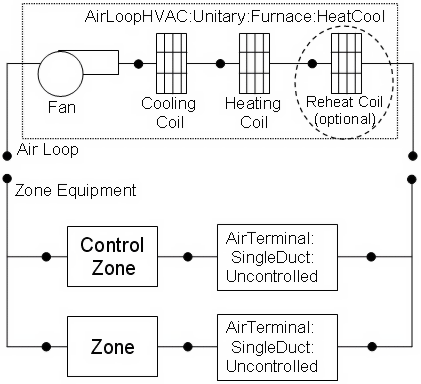
\includegraphics[width=0.9\textwidth, height=0.9\textheight, keepaspectratio=true]{media/image298.png}
\caption{Schematic of EnergyPlus Heat/Cool Furnace \protect \label{fig:schematic-of-energyplus-heatcool-furnace}}
\end{figure}

Note: the coil order shown here has been revised from previous versions (prior to V4.0) of Energyplus to configure the cooling coil upstream of the heating coil. This configuration provides uniformity with all unitary equipment. However, for unitary HeatCool systems that do not use a reheat coil, the heating coil can also be placed upstream of the cooling coil. This optional coil placement is retained to allow compatibility with previous versions of Energyplus. For input files developed using previous versions of Energyplus, it is recommended that the coil order be revised according to the figure above.

Links to the fan, heating coil, DX cooling coil and optional reheat coil specifications are provided in the furnace input data syntax. In addition, the control zone name and the furnace design operating conditions are specified by the furnace inputs.

\subsubsection{Inputs}\label{inputs-2-043}

\paragraph{Field: Name}\label{field-name-2-040}

This alpha field contains the identifying name for the unit.

\paragraph{Field: Availability Schedule Name}\label{field-availability-schedule-name-1-012}

This alpha field contains the schedule name which contains information on the availability of the furnace to operate. A schedule value equal to 0 denotes that the furnace must be off for that time period. A value greater than 0 denotes that the furnace is available to operate during that time period. This schedule may be used to completely disable the furnace as required. If this field is left blank, the schedule has a value of 1 for all time periods.

\paragraph{Field: Furnace Air Inlet Node Name}\label{field-furnace-air-inlet-node-name}

This alpha field contains the furnace inlet node name.

\paragraph{Field: Furnace Air Outlet Node Name}\label{field-furnace-air-outlet-node-name}

This alpha field contains the furnace outlet node name.

\paragraph{Field: Supply Air Fan Operating Mode Schedule Name}\label{field-supply-air-fan-operating-mode-schedule-name}

This alpha field specifies the name of the supply air fan operating mode schedule. The supply air fan operating mode may vary during the simulation based on time-of-day or with a change of season. Schedule values of 0 denote that the furnace supply air fan and the heating or cooling coil cycle on and off together to meet the heating or cooling load (a.k.a. AUTO fan). Schedule values other than 0 denote that the supply fan runs continuously while the heating or cooling coil cycles to meet the load.

\paragraph{Field: Maximum Supply Air Temperature}\label{field-maximum-supply-air-temperature-1-000}

This numeric field contains the design operating furnace air outlet temperature in degrees C when the furnace is heating. If this input field is left blank, the default value is 80 C.

\paragraph{Field: Cooling Supply Air Flow Rate}\label{field-cooling-supply-air-flow-rate-1-000}

This numeric field defines the supply air flow rate leaving the furnace in cubic meters per second when the DX cooling coil is operating. Values must be greater than 0 or this field is autosizable.

\paragraph{Field: Heating Supply Air Flow Rate}\label{field-heating-supply-air-flow-rate-1-000}

This numeric field defines the supply air flow rate leaving the furnace in cubic meters per second when the DX heating coil and/or supplemental heater are operating. Values must be greater than 0 or this field is autosizable.

\paragraph{Field: No Load Supply Air Flow Rate}\label{field-no-load-supply-air-flow-rate-1-000}

This numeric field defines the supply air flow rate leaving the furnace in cubic meters per second when neither cooling or heating is required (i.e., DX coils and supplemental heater are off but the supply air fan operates). This field is only used when the furnace operating mode is specified as continuous fan operation. Values must be greater than or equal to zero, or this field is autosizable. If the furnace operating mode is specified as continuous fan operation and this value is set to zero or this field is left blank, then the model assumes that the supply air flow rate when no cooling/heating is needed is equal to the supply air flow rate when the compressor was last operating (for cooling operation or heating operation).

\paragraph{Field: Controlling Zone or Thermostat Location}\label{field-controlling-zone-or-thermostat-location-1}

This alpha field contains the identifying zone name where the thermostat controlling the furnace is located.

\paragraph{Field: Supply Fan Object Type}\label{field-supply-fan-object-type-1}

This alpha field contains the identifying type of supply air fan specified for the furnace. Fan type must be \textbf{\hyperref[fanonoff]{Fan:OnOff}} or \textbf{\hyperref[fanconstantvolume]{Fan:ConstantVolume}}. \hyperref[fanconstantvolume]{Fan:ConstantVolume} is used when the Supply Air Fan Operating Mode Schedule values are never 0 and the fan operates continuously. \hyperref[fanonoff]{Fan:OnOff} is used when the fan cycles on and off with the cooling or heating coil (i.e.~Supply Air Fan Operating Mode Schedule values are at times 0).

\paragraph{Field: Supply Fan Name}\label{field-supply-fan-name-1}

This alpha field contains the identifying name given to the furnace fan.

\paragraph{Field: Fan Placement}\label{field-fan-placement-1}

This alpha field has two choices: \textbf{BlowThrough} or \textbf{DrawThrough}. The first choice stands for ``blow through fan''. This means that the unit consists of a fan followed by the DX coils and supplemental heating coil. The fan ``blows through'' the cooling and heating coils. The second choice stands for ``draw through fan''. This means that the unit consists of the DX coil(s) followed by a fan, with the supplemental heater located at the outlet of the fan. The fan ``draws air through'' the DX coil(s). If this field is left blank, the default is blow through.

\paragraph{Field: Heating Coil Object Type}\label{field-heating-coil-object-type-1-000}

This alpha field contains the identifying type of heating coil specified in the furnace. The hot water and steam heating coils require specifying plant loop, branches, and connector objects to support the heating coils, and are placed on the demand side of the plantloop. The hot water flow modulation through the heating coil does not require additional controller or \hyperref[controllerwatercoil]{Controller:WaterCoil} object. The parent object (Unitary Heat and Cool Furnace) itself provides the ``controller'' function of modulating water flow. Allowable coil types are:

\begin{itemize}
\item
  \hyperref[coilheatingelectric]{Coil:Heating:Electric}
\item
  \hyperref[coilheatinggas-000]{Coil:Heating:Fuel}
\item
  \hyperref[coilheatingwater]{Coil:Heating:Water}
\item
  \hyperref[coilheatingsteam]{Coil:Heating:Steam}
\end{itemize}

\paragraph{Field: Heating Coil Name}\label{field-heating-coil-name-1-000}

This alpha field contains the identifying name given to the furnace heating coil.

\paragraph{Field: Cooling Coil Object Type}\label{field-cooling-coil-object-type-1-000}

This alpha field contains the identifying type of cooling coil specified in the furnace. Only allowable coil types are:

\begin{itemize}
\item
  \hyperref[coilcoolingdxsinglespeed]{Coil:Cooling:DX:SingleSpeed}
\item
  \hyperref[coilsystemcoolingdxheatexchangerassisted]{CoilSystem:Cooling:DX:HeatExchangerAssisted}
\item
  \hyperref[coilcoolingdxvariablespeed]{Coil:Cooling:DX:VariableSpeed}
\end{itemize}

\paragraph{Field: Cooling Coil Name}\label{field-cooling-coil-name-1-000}

This alpha field contains the identifying name given to the furnace cooling coil.

\paragraph{Field: Dehumidification Control Type}\label{field-dehumidification-control-type-1-000}

This alpha field contains the type of dehumidification control. The following options are valid for this field:

\begin{itemize}
\item
  \textbf{None} - meet sensible load only, no active dehumidification control
\item
  \textbf{Multimode} - activate enhanced dehumidification mode as needed and meet sensible load. This option is used to model DX equipment with a controllable heat exchanger assisting the DX cooling coil for improved dehumidification. It is valid only with cooling coil type = \hyperref[coilsystemcoolingdxheatexchangerassisted]{CoilSystem:Cooling:DX:HeatExchangerAssisted}.
\item
  \textbf{CoolReheat} - cool beyond the dry-bulb temperature set point as required to meet the high humidity setpoint. If cooling coil type = \hyperref[coilsystemcoolingdxheatexchangerassisted]{CoilSystem:Cooling:DX:HeatExchangerAssisted}, then the heat exchanger is assumed to always transfer energy between the cooling coil's inlet and outlet airstreams when the cooling coil is operating.
\end{itemize}

The default is \textbf{None}. For the other dehumidification control modes, the maximum humidity setpoint is used. This must be set using a \textbf{\hyperref[zonecontrolhumidistat]{ZoneControl:Humidistat}} object. When extra dehumidification is required, the system may not be able to meet the humidity setpoint if its full capacity is not adequate. If the dehumidification control type is specified as \textbf{CoolReheat}, then two additional inputs (reheat coil type and name) are also required as shown below. Although the reheat coil is required only when \textbf{CoolRheat} is selected, the optional reheat coil may be present for any of the allowed Dehumidification Control Types. If the reheat coil is present and the dehumidification control type is not specified as \textbf{CoolReheat}, the reheat coil will not be active,

\paragraph{Field: Reheat Coil Object Type}\label{field-reheat-coil-object-type-000}

This alpha field contains the identifying type of reheat coil specified in the furnace. The hot water and steam heating coils require specifying plant loop, branches, and connector objects to support the heating coils, and are placed on the demand side of the plantloop. The hot water flow modulation through the reheat coil does not require additional controller or \hyperref[controllerwatercoil]{Controller:WaterCoil} object. The parent object (Unitary Heat and Cool Furnace) itself provides the ``controller'' function of modulating water flow. Reheat coil type must be one of:

\begin{itemize}
\item
  \hyperref[coilheatingelectric]{Coil:Heating:Electric}
\item
  \hyperref[coilheatinggas-000]{Coil:Heating:Fuel}
\item
  \hyperref[coilheatingdesuperheater]{Coil:Heating:Desuperheater}
\item
  \hyperref[coilheatingwater]{Coil:Heating:Water}
\item
  \hyperref[coilheatingsteam]{Coil:Heating:Steam}
\end{itemize}

\paragraph{Field: Reheat Coil Name}\label{field-reheat-coil-name-000}

This alpha field contains the identifying name given to the furnace reheat coil.

As shown in the example below, correct specification of the heat/cool furnace requires specification of the following objects in addition to the furnace object:

\begin{enumerate}
\def\labelenumi{\arabic{enumi})}
\item
  fan (\hyperref[fanonoff]{Fan:OnOff} or \hyperref[fanconstantvolume]{Fan:ConstantVolume})
\item
  cooling coil (\hyperref[coilcoolingdxsinglespeed]{Coil:Cooling:DX:SingleSpeed} or \hyperref[coilsystemcoolingdxheatexchangerassisted]{CoilSystem:Cooling:DX:HeatExchangerAssisted})
\item
  heating coil (\hyperref[coilheatinggas-000]{Coil:Heating:Fuel} or \hyperref[coilheatingelectric]{Coil:Heating:Electric})
\item
  reheat coil (optional, \hyperref[coilheatinggas-000]{Coil:Heating:Fuel}, \hyperref[coilheatingelectric]{Coil:Heating:Electric}, or \hyperref[coilheatingdesuperheater]{Coil:Heating:Desuperheater})
\item
  terminal unit (\hyperref[airterminalsingleductconstantvolumenoreheat]{AirTerminal:SingleDuct:ConstantVolume:NoReheat}) for each zone served by the furnace
\end{enumerate}

Note: the furnace's fan, cooling coil, heating coil and optional reheat coil must be connected in the air loop according to the configuration shown above (Figure~\ref{fig:schematic-of-energyplus-heatcool-furnace}) when CoolReheat is selected as the dehujmidificaiton control type. In addition, the volumetric air flow rate specified in the terminal air unit for the controlling zone should properly reflect the fractional volumetric air flow rate specified in the furnace object.

\begin{lstlisting}

AirLoopHVAC:Unitary:Furnace:HeatCool,
  GasHeat DXAC Furnace 1, !- Name of furnace
  FanAndCoilAvailSched,   !- Availability schedule
  Air Loop Inlet Node,    !- Furnace inlet node name
  Air Loop Outlet Node,   !- Furnace outlet node name
  CycFanSchedule,         !- Supply Air Fan Operating Mode Schedule Name
  80,                     !- Maximum supply air temperature from furnace heater {C}
  1.3,                    !- Cooling Supply Air Flow Rate {m3/s}
  1.3,                    !- Heating Supply Air Flow Rate {m3/s}
  0.0,                    !- No Load Supply Air Flow Rate {m3/s}
  East Zone,              !- Controlling zone or thermostat location
  Fan:OnOff,              !- Supply fan type
  Supply Fan 1,           !- Supply fan name
  BlowThrough,            !- Fan Placement
  Coil:Heating:Fuel,       !- Heating coil type
  Furnace Heating Coil 1, !- Heating coil name
  Coil:Cooling:DX:SingleSpeed,  !- Cooling coil type
  Furnace ACDXCoil 1,     !- Cooling coil name
  None;                   !- Dehumidificatioin Control Type


  Coil:Heating:Fuel,
      Furnace Heating Coil 1,         !- Coil Name
      FanAndCoilAvailSched,           !- Availability Schedule Name
      NaturalGas,                     !- Fuel Type
      0.8,    !- Gas Burner Efficiency of the Coil
      25000,  !- Nominal Capacity of the Coil {W}
      Heating Coil Air Inlet Node,    !- Coil\_Air\_Inlet\_Node
      Air Loop Outlet Node;           !- Coil\_Air\_Outlet\_Node

    Coil:Cooling:DX:SingleSpeed,
      Furnace ACDXCoil 1,    !- Coil Name
      FanAndCoilAvailSched,  !- Availability Schedule
      25000,  !- Rated Total Cooling Capacity (gross) {W}
      0.75,   !- Rated SHR
      3.0,    !- Rated COP
      1.3,    !- Rated Air Volume Flow Rate {m3/s}
      DX Cooling Coil Air Inlet Node, !- Coil Air Inlet Node
      Heating Coil Air Inlet Node,    !- Coil Air Outlet Node
      WindACCoolCapFT,  !- Total Cooling Capacity Modifier Curve (function of temperature)
      WindACCoolCapFFF, !- Total Cooling Capacity Modifier Curve (function of flow fraction)
      WindACEIRFT,      !- Energy Input Ratio Modifier Curve (function of temperature)
      WindACEIRFFF,     !- Energy Input Ratio Modifier Curve (function of flow fraction)
      WindACPLFFPLR,    !- Part Load Fraction Correlation (function of part load ratio)
      CyclingFanAndCompressor;    !- Supply Air Fan Operation Mode

    Fan:OnOff,
      Supply Fan 1,                !- Fan Name
      FanAndCoilAvailSched,        !- Availability Schedule Name
      0.7,    !- Fan Total Efficiency
      600.0,  !- Delta Pressure {Pa}
      1.3,    !- Max Flow Rate {m3/s}
      0.9,    !- Motor Efficiency
      1.0,    !- Motor In Airstream Fraction
      Air Loop Inlet Node,         !- Fan\_Inlet\_Node
      DX Cooling Coil Air Inlet Node; !- Fan\_Outlet\_Node

    AirTerminal:SingleDuct:ConstantVolume:NoReheat,
      Zone1DirectAir,              !- Name
      ,                            !- Availability Schedule Name
      Zone 1 Terminal Inlet Node,  !- Air Inlet Node Name
      Zone 1 Supply Node,          !- Air Outlet Node Name
      0.47;                        !- Maximum air flow rate {m3/s}

    AirTerminal:SingleDuct:ConstantVolume:NoReheat,
      Zone2DirectAir,              !- Name
      ,                            !- Availability Schedule Name
      Zone 2 Terminal Inlet Node,  !- Air Inlet Node Name
      Zone 2 Supply Node,          !- Air Outlet Node Name
      0.36;                        !- Maximum air flow rate {m3/s}

    AirTerminal:SingleDuct:ConstantVolume:NoReheat,
      Zone3DirectAir,              !- Name
      ,                            !- Availability Schedule Name
      Zone 3 Terminal Inlet Node,  !- Air Inlet Node Name
      Zone 3 Supply Node,          !- Air Outlet Node Name
      0.47;                        !- Maximum air flow rate {m3/s}
\end{lstlisting}

~Example of Heat/Cool Furnace Specification

\subsubsection{Outputs}\label{outputs-1-029}

HVAC,Average,Unitary System Fan Part Load Ratio {[]}

HVAC,Average,Unitary System Compressor Part Load Ratio {[]}

\paragraph{Unitary System Fan Part Load Ratio}\label{unitary-system-fan-part-load-ratio-1}

This output variable is the ratio of actual air mass flow rate through the furnace to the furnace's design air mass flow rate (i.e., design volumetric flow rate converted to dry air mass flow rate). For continuous fan operation mode, this variable is always 1.0 when the furnace is available (based on the availability schedule). For cycling fan/cycling coil operation mode, the actual air mass flow rate is calculated based on the ratio of the sensible heating (or cooling) load to the steady-state furnace heating (or cooling) capacity. For the cycling fan mode, the runtime fraction for the furnace fan may be different from the fan part-load ratio reported here due the part-load performance of the furnace's heating (or cooling) coil (delay at start-up to reach steady-state output). In general, runtime fractions are reported by individual components where appropriate (e.g., Fan:OnOff).

Unitary System Compressor Part Load Ratio {[]}

\subsection{AirLoopHVAC:UnitaryHeatCool}\label{airloophvacunitaryheatcool}

The AirLoopHVAC:UnitaryHeatCool object is the identical model to the AirLoopHAVC:Unitary:Furnace:HeatCool object. The heat/cool unitary system is a ``virtual'' component that consists of a fan component (OnOff or ConstantVolume), a DX cooling coil component and a Gas or Electric heating coil component as shown in Figure~\ref{fig:schematic-of-blow-through-heatcool-unitary}. When a draw through configuration is desired, the fan is placed directly after the heating coil. If dehumidification control is selected, a reheat coil component is also required. If the reheat coil is present and the dehumidification control type input is not specified as CoolReheat, the reheat coil will not be active,

\begin{figure}[hbtp] % fig 117
\centering
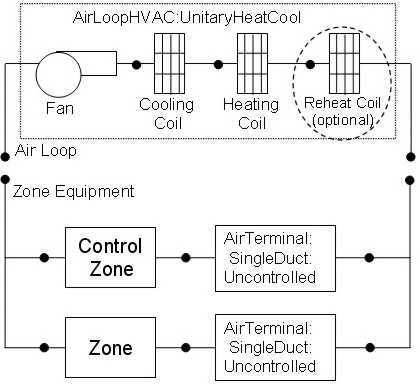
\includegraphics[width=0.9\textwidth, height=0.9\textheight, keepaspectratio=true]{media/image299.png}
\caption{Schematic of Blow Through Heat/Cool Unitary System \protect \label{fig:schematic-of-blow-through-heatcool-unitary}}
\end{figure}

Note: the coil order shown here has been revised from previous versions (prior to V4.0) of Energyplus to configure the cooling coil upstream of the heating coil. This configuration provides uniformity with all unitary equipment. However, for unitary HeatCool systems that do not use a reheat coil, the heating coil can also be placed upstream of the cooling coil. This optional coil placement is retained to allow compatibility with previous versions of Energyplus. For input files developed using previous versions of Energyplus, it is recommended that the coil order be revised according to the figure above.

Links to the fan, DX cooling coil, heating coil and optional reheat coil specifications are provided in the unitary system input data syntax. In addition, the control zone name and the system design operating conditions are specified by the unitary system inputs.

\subsubsection{Field: Name}\label{field-name-3-034}

This alpha field contains the identifying name for the unitary system.

\subsubsection{Field: Availability Schedule Name}\label{field-availability-schedule-name-2-008}

This alpha field contains the schedule name which contains information on the availability of the unitary system to operate. A schedule value equal to 0 denotes that the unitary system must be off for that time period. A value greater than 0 denotes that the unitary system is available to operate during that time period. This schedule may be used to completely disable the unitary system as required. If this field is left blank, the schedule has a value of 1 for all time periods.

\subsubsection{Field: Unitary System Air Inlet Node Name}\label{field-unitary-system-air-inlet-node-name-1}

This alpha field contains the unitary system inlet node name.

\subsubsection{Field: Unitary System Air Outlet Node Name}\label{field-unitary-system-air-outlet-node-name-1}

This alpha field contains the unitary system outlet node name.

\textbf{\emph{Field: Supply Air Fan Operating Mode Schedule Name}}

This alpha field specifies the name of the supply air fan operating mode schedule. The supply air fan operating mode may vary during the simulation based on time-of-day or with a change of season. Schedule values of 0 denote that the unitary system supply air fan and the heating or cooling coil cycle on and off together to meet the heating or cooling load (a.k.a. AUTO fan). Schedule values other than 0 denote that the supply fan runs continuously while the heating or cooling coil cycles to meet the load.

\subsubsection{Field: Maximum Supply Air Temperature}\label{field-maximum-supply-air-temperature-2-000}

This numeric field contains the design operating air outlet temperature in degrees C when the unitary system is heating. If this input field is left blank, the default value is 80 C.

\subsubsection{Field: Cooling Supply Air Flow Rate}\label{field-cooling-supply-air-flow-rate-2-000}

This numeric field defines the supply air flow rate leaving the unitary system in cubic meters per second when the DX cooling coil is operating. Values must be greater than 0 or this field is autosizable.

\subsubsection{Field: Heating Supply Air Flow Rate}\label{field-heating-supply-air-flow-rate-2-000}

This numeric field defines the supply air flow rate leaving the unitary system in cubic meters per second when the DX heating coil and/or supplemental heater are operating. Values must be greater than 0 or this field is autosizable.

\subsubsection{Field: No Load Supply Air Flow Rate}\label{field-no-load-supply-air-flow-rate-2-000}

This numeric field defines the supply air flow rate leaving the unitary system in cubic meters per second when neither cooling or heating is required (i.e., DX coils and supplemental heater are off but the supply air fan operates). This field is only used when the unitary system operating mode is specified as continuous fan operation. Values must be greater than or equal to zero, or this field is autosizable. If the unitary system operating mode is specified as continuous fan operation and this value is set to zero or this field is left blank, then the model assumes that the supply air flow rate when no cooling/heating is needed is equal to the supply air flow rate when the compressor was last operating (for cooling operation or heating operation).

\subsubsection{Field: Controlling Zone or Thermostat Location}\label{field-controlling-zone-or-thermostat-location-2}

This alpha field contains the identifying zone name where the thermostat controlling the unitary system is located.

\subsubsection{Field: Supply Fan Object Type}\label{field-supply-fan-object-type-2}

This alpha field contains the identifying type of supply air fan specified for the unitary system. Fan type must be \textbf{\hyperref[fanonoff]{Fan:OnOff}} or \textbf{\hyperref[fanconstantvolume]{Fan:ConstantVolume}}. \hyperref[fanconstantvolume]{Fan:ConstantVolume} is used when the Supply Air Fan Operating Mode Schedule values are never 0 and the fan operates continuously. \hyperref[fanonoff]{Fan:OnOff} is used when the fan cycles on and off with the cooling or heating coil (i.e.~Supply Air Fan Operating Mode Schedule values are at times 0).

\subsubsection{Field: Supply Fan Name}\label{field-supply-fan-name-2}

This alpha field contains the identifying name given to the unitary system fan.

\subsubsection{Field: Fan Placement}\label{field-fan-placement-2}

This alpha field has two choices: \textbf{BlowThrough} or \textbf{DrawThrough}. The first choice stands for ``blow through fan''. This means that the unit consists of a fan followed by the DX coils and supplemental heating coil. The fan ``blows through'' the cooling and heating coils. The second choice stands for ``draw through fan''. This means that the unit consists of the DX coil(s) followed by a fan, with the supplemental heater located at the outlet of the fan. The fan ``draws air through'' the DX coil(s). If this field is left blank, the default is blow through.

\subsubsection{Field: Heating Coil Object Type}\label{field-heating-coil-object-type-2}

This alpha field contains the identifying type of heating coil specified in the unitary system. The hot water and steam heating coils require specifying plant loop, branches, and connector objects to support the heating coils, and are placed on the demand side of the plantloop. The hot water flow modulation through the heating coil does not require additional controller or \hyperref[controllerwatercoil]{Controller:WaterCoil} object. The parent object (Unitary Heat and Cool System) itself provides the ``controller'' function of modulating water flow. Allowable coil types are:

\begin{itemize}
\item
  \hyperref[coilheatingelectric]{Coil:Heating:Electric}
\item
  \hyperref[coilheatinggas-000]{Coil:Heating:Fuel}
\item
  \hyperref[coilheatingwater]{Coil:Heating:Water}
\item
  \hyperref[coilheatingsteam]{Coil:Heating:Steam}
\end{itemize}

\subsubsection{Field: Heating Coil Name}\label{field-heating-coil-name-2}

This alpha field contains the identifying name given to the unitary system heating coil.

\subsubsection{Field: Cooling Coil Object Type}\label{field-cooling-coil-object-type-2-000}

This alpha field contains the identifying type of cooling coil specified in the unitary system. Only allowable coil types are:

\begin{itemize}
\item
  \hyperref[coilcoolingdxsinglespeed]{Coil:Cooling:DX:SingleSpeed}
\item
  \hyperref[coilsystemcoolingdxheatexchangerassisted]{CoilSystem:Cooling:DX:HeatExchangerAssisted}
\item
  \hyperref[coilcoolingdxvariablespeed]{Coil:Cooling:DX:VariableSpeed}
\end{itemize}

\subsubsection{Field: Cooling Coil Name}\label{field-cooling-coil-name-2-000}

This alpha field contains the identifying name given to the unitary system cooling coil.

\subsubsection{Field: Dehumidification Control Type}\label{field-dehumidification-control-type-2-000}

This alpha field contains the type of dehumidification control. The following options are valid for this field:

\begin{itemize}
\item
  \textbf{None} - meet sensible load only, no active dehumidification control
\item
  \textbf{Multimode} - activate enhanced dehumidification mode as needed and meet sensible load. This option is used to model DX equipment with a controllable heat exchanger assisting the DX cooling coil for improved dehumidification. It is valid only with cooling coil type = \hyperref[coilsystemcoolingdxheatexchangerassisted]{CoilSystem:Cooling:DX:HeatExchangerAssisted}.
\item
  \textbf{CoolReheat} - cool beyond the dry-bulb temperature set point as required to meet the high humidity setpoint. If cooling coil type = \hyperref[coilsystemcoolingdxheatexchangerassisted]{CoilSystem:Cooling:DX:HeatExchangerAssisted}, then the heat exchanger is assumed to always transfer energy between the cooling coil's inlet and outlet airstreams when the cooling coil is operating.
\end{itemize}

The default is \textbf{None}. For the other dehumidification control modes, the maximum humidity setpoint is used. This must be set using a \textbf{\hyperref[zonecontrolhumidistat]{ZoneControl:Humidistat}} object. When extra dehumidification is required, the system may not be able to meet the humidity setpoint if its full capacity is not adequate. If the dehumidification control type is specified as \textbf{CoolReheat}, then two additional inputs (reheat coil type and name) are also required as shown below. Although the reheat coil is required only when \textbf{CoolReheat} is selected, the optional reheat coil may be present for any of the allowed Dehumidification Control Types. If the reheat coil is present and the dehumidification control type is not specified as \textbf{CoolReheat}, the reheat coil will not be active,

\subsubsection{Field: Reheat Coil Object Type}\label{field-reheat-coil-object-type-1-000}

This alpha field contains the identifying type of reheat coil specified in the unitary system. The hot water and steam heating coils require specifying plant loop, branches, and connector objects to support the heating coils, and are placed on the demand side of the plantloop. The hot water flow modulation through the reheat coil does not require additional controller or \hyperref[controllerwatercoil]{Controller:WaterCoil} object. The parent object (Unitary Heat and Cool System) itself provides the ``controller'' function of modulating water flow. Reheat coil type must be one of:

\begin{itemize}
\item
  \hyperref[coilheatingelectric]{Coil:Heating:Electric}
\item
  \hyperref[coilheatinggas-000]{Coil:Heating:Fuel}
\item
  \hyperref[coilheatingdesuperheater]{Coil:Heating:Desuperheater}
\item
  \hyperref[coilheatingwater]{Coil:Heating:Water}
\item
  \hyperref[coilheatingsteam]{Coil:Heating:Steam}
\end{itemize}

\subsubsection{Field: Reheat Coil Name}\label{field-reheat-coil-name-1-000}

This alpha field contains the identifying name given to the unitary system reheat coil.

As shown in the example below, correct specification of the heat/cool unitary system requires specification of the following objects in addition to the unitary system object:

1)~~~Fan (\hyperref[fanonoff]{Fan:OnOff} or \hyperref[fanconstantvolume]{Fan:ConstantVolume})

2)~~~Cooling coil (\hyperref[coilcoolingdxsinglespeed]{Coil:Cooling:DX:SingleSpeed} or \hyperref[coilsystemcoolingdxheatexchangerassisted]{CoilSystem:Cooling:DX:HeatExchangerAssisted})

3)~~~Heating coil (\hyperref[coilheatinggas-000]{Coil:Heating:Fuel} or \hyperref[coilheatingelectric]{Coil:Heating:Electric})

4)~~~Reheat coil (optional, \hyperref[coilheatinggas-000]{Coil:Heating:Fuel}, \hyperref[coilheatingelectric]{Coil:Heating:Electric}, or \hyperref[coilheatingdesuperheater]{Coil:Heating:Desuperheater})

5)~~~Direct air unit (\hyperref[airterminalsingleductconstantvolumenoreheat]{AirTerminal:SingleDuct:ConstantVolume:NoReheat}) for each zone served by the unitary system

Note: the unitary system's fan, cooling coil, heating coil and optional reheat coil must be connected in the air loop according to the configuration shown above (Figure~\ref{fig:schematic-of-blow-through-heatcool-unitary}). In addition, the volumetric air flow rate specified in the direct air unit for the controlling zone should properly reflect the fractional volumetric air flow rate specified in the unitary system object.

\begin{lstlisting}

AirLoopHVAC:Unitary:Furnace:HeatCool,
  GasHeat DXAC Unitary System 1, !- Name of unitary system
  FanAndCoilAvailSched,   !- Availability schedule
  Air Loop Inlet Node,    !- Unitary system inlet node name
  Air Loop Outlet Node,   !- Unitary system outlet node name
  CycFanSchedule,         !- Supply Air Fan Operating Mode Schedule Name
  80,                     !- Maximum supply air temperature from unitary system heater {C}
  1.3,                    !- Cooling Supply Air Flow Rate {m3/s}
  1.3,                    !- Heating Supply Air Flow Rate {m3/s}
  0.0,                    !- No Load Supply Air Flow Rate {m3/s}
  East Zone,              !- Controlling zone or thermostat location
  Fan:OnOff,              !- Supply fan type
  Supply Fan 1,           !- Supply fan name
  BlowThrough,            !- Fan Placement
  Coil:Heating:Fuel,       !- Heating coil type
  Unitary System Heating Coil 1,   !- Heating coil name
  Coil:Cooling:DX:SingleSpeed,  !- Cooling coil type
  Unitary System ACDXCoil 1,       !- Cooling coil name
  None;        !- High humidity control

    Coil:Heating:Fuel,
      Unitary System Heating Coil 1,  !- Coil Name
      FanAndCoilAvailSched,           !- Availability Schedule Name
      NaturalGas,                     !- Fuel Type
      0.8,    !- Gas Burner Efficiency of the Coil
      25000,  !- Nominal Capacity of the Coil {W}
      Heating Coil Air Inlet Node,    !- Coil\_Air\_Inlet\_Node
      Air Loop Outlet Node;           !- Coil\_Air\_Outlet\_Node


    Coil:Cooling:DX:SingleSpeed,
      Unitary System ACDXCoil 1,      !- Coil Name
      FanAndCoilAvailSched,  !- Availability Schedule
      25000,  !- Rated Total Cooling Capacity (gross) {W}
      0.75,   !- Rated SHR
      3.0,    !- Rated COP
      1.3,    !- Rated Air Volume Flow Rate {m3/s}
      DX Cooling Coil Air Inlet Node, !- Coil Air Inlet Node
      Heating Coil Air Inlet Node,    !- Coil Air Outlet Node
      WindACCoolCapFT,  !- Total Cooling Capacity Modifier Curve (function of temperature)
      WindACCoolCapFFF, !- Total Cooling Capacity Modifier Curve (function of flow fraction)
      WindACEIRFT,      !- Energy Input Ratio Modifier Curve (function of temperature)
      WindACEIRFFF,     !- Energy Input Ratio Modifier Curve (function of flow fraction)
      WindACPLFFPLR,    !- Part Load Fraction Correlation (function of part load ratio)
      CyclingFanAndCompressor;    !- Supply Air Fan Operation Mode


    Fan:OnOff,
      Supply Fan 1,                !- Fan Name
      FanAndCoilAvailSched,        !- Availability Schedule Name
      0.7,    !- Fan Total Efficiency
      600.0,  !- Delta Pressure {Pa}
      1.3,    !- Max Flow Rate {m3/s}
      0.9,    !- Motor Efficiency
      1.0,    !- Motor In Airstream Fraction
      Air Loop Inlet Node,         !- Fan\_Inlet\_Node
      DX Cooling Coil Air Inlet Node; !- Fan\_Outlet\_Node

    AirTerminal:SingleDuct:ConstantVolume:NoReheat,
      Zone1DirectAir,              !- Name
      ,                            !- Availability Schedule Name
      Zone 1 Terminal Inlet Node,  !- Air Inlet Node Name
      Zone 1 Supply Node,          !- Air Outlet Node Name
      0.47;                        !- Maximum air flow rate {m3/s}

    AirTerminal:SingleDuct:ConstantVolume:NoReheat,
      Zone2DirectAir,              !- Name
      ,                            !- Availability Schedule Name
      Zone 2 Terminal Inlet Node,  !- Air Inlet Node Name
      Zone 2 Supply Node,          !- Air Outlet Node Name
      0.36;                        !- Maximum air flow rate {m3/s}

    AirTerminal:SingleDuct:ConstantVolume:NoReheat,
      Zone3DirectAir,              !- Name
      ,                            !- Availability Schedule Name
      Zone 3 Terminal Inlet Node,  !- Air Inlet Node Name
      Zone 3 Supply Node,          !- Air Outlet Node Name
      0.47;                        !- Maximum air flow rate {m3/s}
\end{lstlisting}

Example of Heat/Cool Unitary System Specification

\subsection{Unitary System Heat and Cool (AirLoopHVAC) Outputs}\label{unitary-system-heat-and-cool-airloophvac-outputs}

\begin{itemize}
\item
  HVAC,Average, Unitary System Fan Part Load Ratio {[]}
\item
  HVAC,Average, Unitary System Compressor Part Load Ratio
\end{itemize}

\subsubsection{Unitary System Fan Part Load Ratio {[]}}\label{unitary-system-fan-part-load-ratio-2}

This output variable is the ratio of actual air mass flow rate through the unitary system to the system's design air mass flow rate (i.e., design volumetric flow rate converted to dry air mass flow rate). For continuous fan operation mode, this variable is always 1.0 when the unitary system is available (based on the availability schedule). For cycling fan/cycling coil operation mode, the actual air mass flow rate is calculated based on the ratio of the sensible heating (or cooling) load to the steady-state unitary system heating (or cooling) capacity. For the cycling fan mode, the runtime fraction for the unitary system fan may be different from the fan part-load ratio reported here due the part-load performance of the system's heating (or cooling) coil (delay at start-up to reach steady-state output). In general, runtime fractions are reported by individual components where appropriate (e.g., \hyperref[fanonoff]{Fan:OnOff}).

\subsubsection{Unitary System Compressor Part Load Ratio {[]}}\label{unitary-system-compressor-part-load-ratio-1}

This output variable is the ratio of the sensible cooling load to the steady-state cooling capacity of the unitary system's DX cooling coil. The runtime fraction for the DX cooling coil compressor may be different from the compressor part-load ratio reported here due the part-load performance of the cooling coil (delay at start-up to reach steady-state output). In general, runtime fractions are reported by individual components where appropriate.

\subsection{AirLoopHVAC:UnitaryHeatPump:AirToAir}\label{airloophvacunitaryheatpumpairtoair}

The unitary air-to-air heat pump is a ``virtual'' component that consists of a fan component (OnOff or ConstantVolume), a DX cooling coil component, a DX heating coil component, and a Gas or Electric supplementary heating coil component as shown in the Figure below.

\begin{figure}[hbtp] % fig 118
\centering
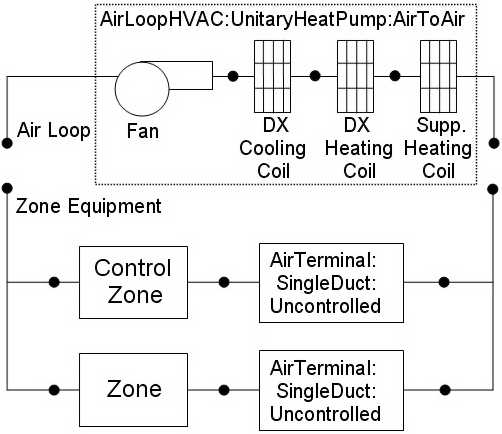
\includegraphics[width=0.9\textwidth, height=0.9\textheight, keepaspectratio=true]{media/image300.png}
\caption{Schematic of EnergyPlus Unitary Air-to-Air Heat Pump (Blow Through Configuration) \label{fig:schematic-of-energyplus-unitary-air-to-air-heat-pump-blow-through-configuration}}
\end{figure}

Links to the fan, DX cooling coil, DX heating coil, and supplementary heating coil specifications are provided in the heat pump's input data syntax. In addition the control zone name and the system design operating conditions are specified by the heat pump inputs.

\subsubsection{Inputs}\label{inputs-3-039}

\paragraph{Field: Name}\label{field-name-4-031}

This alpha field contains the identifying name for the unitary system heat pump.

\paragraph{Field: Availability Schedule Name}\label{field-availability-schedule-name-3-006}

This alpha field contains the schedule name (ref. Schedule objects) that contains information on the availability of the heat pump to operate. A schedule value greater than 0 (usually 1 is used) indicates that the unit can be on during the hour. A value less than or equal to 0 (usually 0 is used) denotes that the unit must be off for the hour. If this field is left blank, the schedule has a value of 1 for all time periods.

\paragraph{Field: Air Inlet Node Name}\label{field-air-inlet-node-name-007}

This alpha field contains the~ name of the HVAC system node from which the heat pump draws its inlet air.

\paragraph{Field: Air Outlet Node Name}\label{field-air-outlet-node-name-006}

This alpha field contains the~ name of the HVAC system node to which the heat pump sends its outlet air.

\paragraph{Field: Cooling Supply Air Flow Rate}\label{field-cooling-supply-air-flow-rate-3-000}

This numeric field defines the supply air flow rate leaving the heat pump in cubic meters per second when the DX cooling coil is operating. Values must be greater than 0 or this field is autosizable.

\paragraph{Field: Heating Supply Air Flow Rate}\label{field-heating-supply-air-flow-rate-3-000}

This numeric field defines the supply air flow rate leaving the heat pump in cubic meters per second when the DX heating coil and/or supplemental heater are operating. Values must be greater than 0 or this field is autosizable.

\paragraph{Field: No Load Supply Air Flow Rate}\label{field-no-load-supply-air-flow-rate-3-000}

This numeric field defines the supply air flow rate leaving the heat pump in cubic meters per second when neither cooling or heating is required (i.e., DX coils and supplemental heater are off but the supply air fan operates). This field is only used when the heat pump operating mode is specified as continuous fan operation. Values must be greater than or equal to zero, or this field is autosizable. If the heat pump operating mode is specified as continuous fan operation and this value is set to zero or this field is left blank, then the model assumes that the supply air flow rate when no cooling/heating is needed is equal to the supply air flow rate when the compressor was last operating (for cooling operation or heating operation).

\paragraph{Field: Controlling Zone or Thermostat Location}\label{field-controlling-zone-or-thermostat-location-3}

This alpha field contains the identifying zone name where the thermostat controlling the heat pump is located.

\paragraph{Field: Supply Air Fan Object Type}\label{field-supply-air-fan-object-type}

This alpha field contains the identifying type of supply air fan specified for the heat pump. Fan type must be \textbf{\hyperref[fanonoff]{Fan:OnOff}} or \textbf{\hyperref[fanconstantvolume]{Fan:ConstantVolume}}. \hyperref[fanconstantvolume]{Fan:ConstantVolume} is used when the Supply Air Fan Operating Mode Schedule values are never 0 and the fan operates continuously. \hyperref[fanonoff]{Fan:OnOff} is used when the fan cycles on and off with the cooling or heating coil (i.e.~Supply Air Fan Operating Mode Schedule values are at times 0).

\paragraph{Field: Supply Air Fan Name}\label{field-supply-air-fan-name}

This alpha field contains the identifying name given to the heat pump supply air fan, and should match the name specified in the corresponding fan object.

\paragraph{Field: Heating Coil Object Type}\label{field-heating-coil-object-type-3}

This alpha field contains the identifying type of heating coil specified in the heat pump. Heating coil type must be either \hyperref[coilheatingdxsinglespeed]{Coil:Heating:DX:SingleSpeed} or \hyperref[coilheatingdxvariablespeed]{Coil:Heating:DX:VariableSpeed}.

\paragraph{Field: Heating Coil Name}\label{field-heating-coil-name-3}

This alpha field contains the identifying name given to the heat pump DX heating coil, and should match the name specified in the corresponding DX heating coil object.

\paragraph{Field: Cooling Coil Object Type}\label{field-cooling-coil-object-type-3}

This alpha field contains the identifying type of cooling coil specified in the heat pump. There are three valid choices for this field:

\begin{itemize}
\item
  \hyperref[coilcoolingdxsinglespeed]{Coil:Cooling:DX:SingleSpeed}
\item
  \hyperref[coilsystemcoolingdxheatexchangerassisted]{CoilSystem:Cooling:DX:HeatExchangerAssisted}
\item
  \hyperref[coilcoolingdxvariablespeed]{Coil:Cooling:DX:VariableSpeed}
\end{itemize}

\paragraph{Field: Cooling Coil Name}\label{field-cooling-coil-name-3}

This alpha field contains the identifying name given to the heat pump cooling coil, and should match the name specified in the corresponding DX cooling coil object.

\paragraph{Field: Supplemental Heating Coil Object Type}\label{field-supplemental-heating-coil-object-type-1}

This alpha field contains the identifying type of supplemental heating coil specified in the heat pump. The hot water and steam heating coils require specifying plant loop, branches, and connector objects to support the heating coils, and are placed on the demand side of the plantloop. The hot water flow modulation through the supplemental heating coil does not require additional controller or \hyperref[controllerwatercoil]{Controller:WaterCoil} object. The parent object (Airloop Air to Air Heat Pump) itself provides the ``controller'' function of modulating water flow. Heating coil type must be:

\begin{itemize}
\item
  \hyperref[coilheatingelectric]{Coil:Heating:Electric}
\item
  \hyperref[coilheatinggas-000]{Coil:Heating:Fuel}
\item
  \hyperref[coilheatingwater]{Coil:Heating:Water}
\item
  \hyperref[coilheatingsteam]{Coil:Heating:Steam}
\end{itemize}

\paragraph{Field: Supplemental Heating Coil Name}\label{field-supplemental-heating-coil-name-1}

This alpha field contains the identifying name given to the heat pump supplemental heating coil, and should match the name specified in the corresponding heating coil object.

\paragraph{Field: Maximum Supply Air Temperature from Supplemental Heater}\label{field-maximum-supply-air-temperature-from-supplemental-heater}

This numeric field defines the maximum allowed supply air temperature exiting the heat pump supplemental heating coil.

\paragraph{Field: Maximum Outdoor Dry-Bulb Temperature for Supplemental Heater Operation}\label{field-maximum-outdoor-dry-bulb-temperature-for-supplemental-heater-operation-1}

This numeric field defines the outdoor air dry-bulb temperature above which the heat pump supplemental heating coil is disabled. The temperature for this input field must be less than or equal to 21 C. If this input field is left blank, the default value is 21 C.

\paragraph{Field: Fan Placement}\label{field-fan-placement-3}

This alpha field has two choices: \textbf{BlowThrough} or \textbf{DrawThrough}. The first choice represents a blow through system where the supply air fan is before the DX cooling/heating coil and the supplementary heating coil. The second choice represents a draw through system where the supply air fan is between the DX cooling/heating coil and the supplementary heating coil. If this input field is left blank, the default is blow through.

\textbf{\emph{Field: Supply Air Fan Operating Mode Schedule Name}}

This alpha field specifies the name of the supply air fan operating mode schedule. The supply air fan operating mode may vary during the simulation based on time-of-day or with a change of season. Schedule values of 0 denote that the unitary system supply air fan and the heating or cooling coil cycle on and off together to meet the heating or cooling load (a.k.a. AUTO fan). Schedule values other than 0 denote that the supply fan runs continuously while the heating or cooling coil cycles to meet the load.

As shown in the example below, correct specification of the air-to-air heat pump requires specification of the following objects in addition to the heat pump object:

1)~~~Fan (\hyperref[fanonoff]{Fan:OnOff} or \hyperref[fanconstantvolume]{Fan:ConstantVolume})

2)~~~Heating coil (\hyperref[coilheatingdxsinglespeed]{Coil:Heating:DX:SingleSpeed})

3)~~~Cooling coil (\hyperref[coilcoolingdxsinglespeed]{Coil:Cooling:DX:SingleSpeed} or \hyperref[coilsystemcoolingdxheatexchangerassisted]{CoilSystem:Cooling:DX:HeatExchangerAssisted})

4)~~~Supplemental heating coil (\hyperref[coilheatinggas-000]{Coil:Heating:Fuel} or \hyperref[coilheatingelectric]{Coil:Heating:Electric})

5)~~~Direct air unit (\hyperref[airterminalsingleductconstantvolumenoreheat]{AirTerminal:SingleDuct:ConstantVolume:NoReheat})for each zone served by the unitary system

\paragraph{Field: Dehumidification Control Type}\label{field-dehumidification-control-type-3-000}

This alpha input field contains the type of dehumidification control. The following options are valid for this field:

\begin{itemize}
\item
  \textbf{None} - meet sensible load only, no active dehumidification control
\item
  \textbf{Multimode} - activate enhanced dehumidification mode as needed and meet sensible cooling load. This option is used to model DX equipment with a controllable heat exchanger assisting the DX cooling coil for improved dehumidification. It is valid only with cooling coil type = \hyperref[coilsystemcoolingdxheatexchangerassisted]{CoilSystem:Cooling:DX:HeatExchangerAssisted}.
\item
  \textbf{CoolReheat} - cool beyond the dry-bulb temperature set point as required to meet the high humidity setpoint. The excess cooling beyond the cooling set point temperature is offset by the supplemental heating coil. If cooling coil type = \hyperref[coilsystemcoolingdxheatexchangerassisted]{CoilSystem:Cooling:DX:HeatExchangerAssisted}, then the heat exchanger is assumed to always transfer energy between the cooling coil's inlet and outlet airstreams when the cooling coil is operating.
\end{itemize}

The default is \textbf{None}. For the other dehumidification control modes, the maximum humidity setpoint is required. This must be set using a \textbf{\hyperref[zonecontrolhumidistat]{ZoneControl:Humidistat}} object. When extra dehumidification is required, the system may not be able to meet the humidity setpoint if its full capacity is not adequate. Supplemental heating coil (supplemental heating coil type and name) is a required input in AirToAir HeatPumps. The supplemental heating coil capacity must be adequate enough to meet the heating coil load and offset the excess cooling load due to extra dehumidification required to meet the high relative humidity setpoint.

Note: the air-to-air heat pump's fan, cooling coil, heating coil and supplementary heating coil must be connected in the air loop according to the configuration shown above (Figure 118) for the blow-through fan configuration. The only other valid configuration is with a draw-through fan placement, where the fan is located between the DX heating coil and the supplementary heating coil.

\paragraph{AirLoopHVAC:UnitaryHeatPump:AirToAir Example Specification}\label{airloophvacunitaryheatpumpairtoair-example-specification}

\begin{lstlisting}

AirLoopHVAC:UnitaryHeatPump:AirToAir,
        DXAC Heat Pump 1,            ! Heat Pump name
        FanAndCoilAvailSched,        ! Heat Pump availability schedule
        Mixed Air Node,              ! Heat Pump air inlet  node
        Air Loop Outlet Node,        ! Heat Pump air outlet  node
        1.3,                  !- Cooling Supply Air Flow Rate {m3/s}
        1.3,                  !- Heating Supply Air Flow Rate {m3/s}
        0.0,                  !- No Load Suuply Air Flow Rate {m3/s}
        East Zone,                   ! Controlling zone or thermostat location
        Fan:OnOff,            ! Supply air fan type
        Supply Fan 1,                ! Supply air fan name –- same name used in fan object
        Coil:Heating:DX:SingleSpeed,    ! Heating coil type
        Heat Pump DX Heating Coil 1, ! Heating coil name –- same name used in DX heating coil object
        Coil:Cooling:DX:SingleSpeed, !  Cooling coil type
        Heat Pump ACDXCoil 1,        ! Cooling coil name –- same name used in DX cooling coil object
        Coil:Heating:Fuel,            ! Supplemental heating coil type
        Heat Pump DX Supp Heating Coil 1, ! Supplemental heating coil name–- same as in heating coil object
        50,                          ! Maximum supply air temperature from supplemental heater [C]
        21,                      ! Maximum outdoor dry-bulb temp for supplemental heating coil operation [C]
        BlowThrough,                ! Fan  placement
        CycFanSchedule,              ! Supply air fan operating mode schedule name
        CoolReheat;                  !- Dehumidification Control Type

     Coil:Heating:DX:SingleSpeed,
        Heat Pump DX Heating Coil 1,     ! Name of heating coil
        FanAndCoilAvailSched,            ! Heating coil schedule
        35000,                           ! Rated total heating capacity [W] (at 21.11C/8.33C)
        2.75,                            ! Rated heating COP
        1.7,                             ! Rated air flow rate [m3/s]
        Heating Coil Air Inlet Node,     ! Coil air inlet node
        SuppHeating Coil Air Inlet Node, ! Coil air outlet node
        HPACHeatCapFT,                   ! Heating capacity modifier curve (temperature,C)
        HPACHeatCapFFF,                  ! Heating capacity modifier curve (flow fraction)
        HPACHeatEIRFT,                   ! Energy input ratio modifier curve (temperature,C)
        HPACHeatEIRFFF,                  ! Energy input ratio modifier curve (flow fraction)
        HPACCoolPLFFPLR,                 ! Part load fraction modifier curve (function of part-load ratio)
        ,                         ! defrost EIR modifier curve (temp, C) not required for resistive defrost
        CyclingFanAndCompressor,                   ! Operation mode (cycling fan, cycling compressor)
        -5.0,                            ! Minimum OAT for heat pump compressor operation [C]
        5.0,                             ! Maximum outdoor dry-bulb temp for defrost operation [C]
        200.0,                           ! Crankcase heater capacity[W]
        10.0,                            ! Maximum OAT for crankcase heater operation [C]
        resistive,                       ! Defrost strategy (resistive or reverse-cycle)
        timed,                           ! Defrost control (timed or on-demand)
        0.166667,                        !Defrost time period fraction (used for timed defrost control only)
        20000;                           ! Resistive defrost heater capacity [W]

     Coil:Cooling:DX:SingleSpeed,
        Heat Pump ACDXCoil 1,            ! Name of cooling coil
        FanAndCoilAvailSched,            ! Availability schedule
        32000,                           ! Rated total cooling capacity [W]
        0.75,                            ! Rated sensible heat ratio
        3.0,                             ! Rated COP
        1.7,                             ! Rated air flow rate [m3/s]
        DX Cooling Coil Air Inlet Node,  ! Coil air inlet node
        Heating Coil Air Inlet Node,     ! Coil air outlet node
        HPACCoolCapFT,                   ! Cooling capacity modifier curve (temperature,C)
        HPACCoolCapFFF,                  ! Cooling capacity modifier curve (flow fraction)
        HPACCoolEIRFT,                   ! Energy input ratio modifier curve (temperature,C)
        HPACCoolEIRFFF,                  ! Energy input ratio modifier curve (flow fraction)
        HPACCoolPLFFPLR,                 ! Part load factor modifier curve (function of part-load ratio)
        CyclingFanAndCompressor;                   ! Operation mode (cycling fan, cycling compressor)

     Coil:Heating:Fuel,
        Heat Pump DX Supp Heating Coil 1, ! Name of heating coil
        FanAndCoilAvailSched,             ! Availability schedule
        NaturalGas,                       ! Fuel Type
        0.8 ,                             ! Gas Burner Efficiency of the Coil
        32000,                            ! Nominal Capacity of the Coil [W]
        SuppHeating Coil Air Inlet Node,  ! Supplementary heating coil air side inlet node
        Air Loop Outlet Node;             ! Supplementary heating coil air side outlet node

     Fan:OnOff,
        Supply Fan 1,                    ! Fan Name
        FanAndCoilAvailSched,            ! Fan Schedule
        0.7,                             ! Fan Total Efficiency
        300.0,                           ! Delta Pressure [N/M^2]
        1.7,                             ! Max Vol Flow Rate  [m^3/Sec]
        0.9,                             ! motor efficiency
        1.0,                             ! motor in air stream fraction
        Mixed Air Node,                  ! fan inlet node
        DX Cooling Coil Air Inlet Node;  ! fan outlet node

    AirTerminal:SingleDuct:ConstantVolume:NoReheat,
      Zone1DirectAir,              !- Name
      ,                            !- Availability Schedule Name
      Zone 1 Terminal Inlet Node,  !- Air Inlet Node Name
      Zone 1 Supply Node,          !- Air Outlet Node Name
      0.612;                       !- Maximum air flow rate {m3/s}

    AirTerminal:SingleDuct:ConstantVolume:NoReheat,
      Zone2DirectAir,              !- Name
      ,                            !- Availability Schedule Name
      Zone 2 Terminal Inlet Node,  !- Air Inlet Node Name
      Zone 2 Supply Node,          !- Air Outlet Node Name
      0.476;                       !- Maximum air flow rate {m3/s}

    AirTerminal:SingleDuct:ConstantVolume:NoReheat,
      Zone3DirectAir,              !- Name
      ,                            !- Availability Schedule Name
      Zone 3 Terminal Inlet Node,  !- Air Inlet Node Name
      Zone 3 Supply Node,          !- Air Outlet Node Name
      0.612;                       !- Maximum air flow rate {m3/s}
\end{lstlisting}

\subsubsection{Outputs}\label{outputs-2-024}

\begin{itemize}
\item
  HVAC, Average, Unitary System Fan Part Load Ratio {[]}
\item
  HVAC, Average, Unitary System Compressor Part Load Ratio {[]}
\item
  HVAC, Average, Unitary System Dehumidification Induced Heating Demand Rate {[}W{]}
\end{itemize}

\paragraph{Unitary System Fan Part Load Ratio {[]}}\label{unitary-system-fan-part-load-ratio-3}

This output variable is the ratio of actual air mass flow rate through the heat pump to the heat pump's design air mass flow rate (i.e., design volumetric flow rate converted to dry air mass flow rate). For continuous fan operation mode, this variable is always 1.0 when the furnace is available (based on the availability schedule). For cycling fan/cycling coil operation mode, the actual air mass flow rate is calculated based on the ratio of the sensible heating (or cooling) load to the steady-state heat pump heating (or cooling) capacity. For the cycling fan mode, the runtime fraction for the heat pump fan may be different from the fan part-load ratio reported here due the part-load performance of the heat pump's heating (or cooling) coil (delay at start-up to reach steady-state output). In general, runtime fractions are reported by individual components where appropriate (e.g., Fan:OnOff).

\paragraph{Unitary System Compressor Part Load Ratio {[]}}\label{unitary-system-compressor-part-load-ratio-2}

This output variable is the ratio of the sensible load (heating or cooling) to the steady-state capacity of the heat pump's DX heating or cooling coil. The runtime fraction for the heat pump compressor may be different from the compressor part-load ratio reported here due the part-load performance of the heating/cooling coil (delay at start-up to reach steady-state output). In general, runtime fractions are reported by individual components where appropriate.

\paragraph{Unitary System Dehumidification Induced Heating Demand Rate {[}W{]}}\label{unitary-system-dehumidification-induced-heating-demand-rate-w}

This output variable is the additional heating demand rate of the supplemental heating coil of an Air-to-Air heat pumps in Watts.~ This additional heating demand is induced when zone air overshoots the heating setpoint due to extra dehumidification requirement to meet the high humidity setpoint. This value is always positive. This value is calculated for each HVAC system timestep, and the results are averaged for the timestep being reported.

\subsection{AirLoopHVAC:UnitaryHeatPump:AirToAir:MultiSpeed}\label{airloophvacunitaryheatpumpairtoairmultispeed}

The multispeed air-to-air heat pump is a ``virtual'' component that consists of a fan component (On/Off or ConstVolume), a DX multispeed cooling coil component, a DX multispeed heating coil component, and a Gas or Electric supplemental heating coil component. This system also includes the option to use available waste energy to heat water. A schematic diagram of the air-to-air multispeed heat pump is shown below. The component connection sequence for the blow through option (shown below) from inlet to outlet is fan, cooling coil, heating coil, and supplemental heater. The connection sequence for the draw through option is cooling coil, heating coil, fan, and supplemental heater.

The main difference between this heat pump object and other EnergyPlus heat pump objects is that this object allows from two to four discrete compressor speeds for heating and cooling operation (instead of a single speed for each mode). The lowest speed is called Speed 1, and the highest speed is called Speed n (2, 3 or 4 as specified in the input syntax). This object allows a different number of speeds for cooling and heating, and each speed has an associated airflow rate. The airflow rates for the various heating speeds can be different from the airflow rates for the cooling speeds. In addition, the airflow rate when no cooling or heating is needed can also be defined. The number of cooling and heating speeds defined by the user in this heat pump object must equal the number of speeds defined in the associated coils (child objects). For example, the number of speeds for cooling defined in this heat pump object must be equal to the number of speeds defined in the associated cooling coil object.

Links to the fan, DX multispeed cooling coil, DX multispeed heating coil, and supplementary heating coil specifications are provided in the heat pump's input data syntax. In addition, the control zone name and airflow rates at the corresponding compressor speeds are specified by the heat pump syntax.

If the \hyperref[zonecontrolthermostatstageddualsetpoint]{ZoneControl:Thermostat:StagedDualSetpoint} object and other zone control thermostat and humidistat are assigned to the same controlled zone in the Controlling Zone or Thermostat Location field, the \hyperref[zonecontrolthermostatstageddualsetpoint]{ZoneControl:Thermostat:StagedDualSetpoint} object takes precedence and the stage number provided by the the \hyperref[zonecontrolthermostatstageddualsetpoint]{ZoneControl:Thermostat:StagedDualSetpoint} object is used to set the speed number.

\begin{figure}[hbtp] % fig 119
\centering
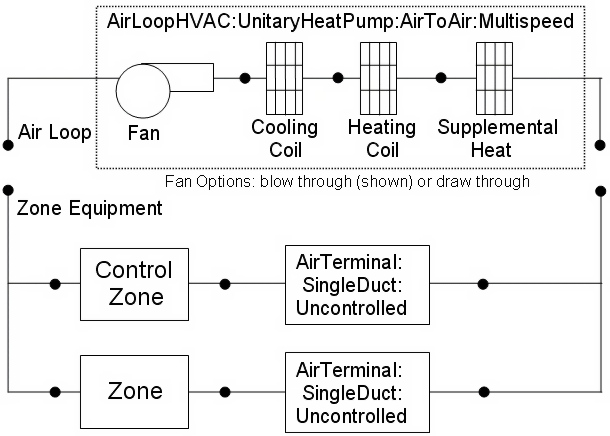
\includegraphics[width=0.9\textwidth, height=0.9\textheight, keepaspectratio=true]{media/image301.png}
\caption{Schematic of EnergyPlus Unitary Air-to-Air Multi Speed Heat Pump \protect \label{fig:schematic-of-energyplus-unitary-air-to-air}}
\end{figure}

\subsubsection{Inputs}\label{inputs-4-036}

\paragraph{Field: Name}\label{field-name-5-027}

This alpha field contains the identifying name for the multispeed heat pump.

\paragraph{Field: Availability Schedule Name}\label{field-availability-schedule-name-4-006}

This alpha field contains the schedule name (ref. Schedule objects) that contains information on the availability of the heat pump to operate. A schedule value greater than 0 (usually 1 is used) indicates that the unit can be on during the time period. A value less than or equal to 0 (usually 0 is used) denotes that the unit must be off for the time period. If this field is left blank, the schedule has a value of 1 for all time periods.

\paragraph{Field: Air Inlet Node Name}\label{field-air-inlet-node-name-1-005}

This alpha field contains the name of the HVAC system node from which the heat pump draws its inlet air.

\paragraph{Field: Air Outlet Node Name}\label{field-air-outlet-node-name-1-004}

This alpha field contains the name of the HVAC system node to which the heat pump sends its outlet air.

\paragraph{Field: Controlling Zone or Thermostat Location}\label{field-controlling-zone-or-thermostat-location-4}

This alpha field contains the identifying zone name where the thermostat controlling the multispeed heat pump is located.

\paragraph{Field: Supply Air Fan Object Type}\label{field-supply-air-fan-object-type-1}

This alpha field contains the identifying type of supply air fan specified for the heat pump. Fan type must be \hyperref[fanonoff]{Fan:OnOff} or \hyperref[fanconstantvolume]{Fan:ConstantVolume}. \hyperref[fanconstantvolume]{Fan:ConstantVolume} can only be used when the supply air fan operating mode is continuous (see field `Supply air fan operating mode schedule name).

\paragraph{Field: Supply Air Fan Name}\label{field-supply-air-fan-name-1}

This alpha field contains the identifying name given to the heat pump supply air fan, and should match the name specified in the corresponding fan object.

\paragraph{Field: Supply Air Fan Placement}\label{field-supply-air-fan-placement}

This alpha field has two choices: \textbf{BlowThrough} or \textbf{DrawThrough}. The first choice stands for ``blow through fan''. This means that the unit consists of a fan followed by a DX multispeed cooling coil, DX multispeed heating coil, and a supplemental heating coil. The fan ``blows through'' the cooling and heating coils. The second choice stands for ``draw through fan''. This means that the unit consists of the DX cooling and heating coils followed by a fan, with the supplemental heater located at the outlet of the fan.~ The fan ``draws'' air through the DX coils.

\textbf{Note}: the multispeed heat pump's supply air fan, cooling coil, heating coil and supplemental heating coil must be connected according to the configuration shown above (Figure~\ref{fig:schematic-of-energyplus-unitary-air-to-air}) for the `blow through' fan configuration. For the `draw through' fan configuration the fan must be located between the DX heating coil and the supplemental heater, whose outlet node is the system outlet node. In addition, the DX cooling coil and DX heating coil operation mode must be specified consistently with the heat pump's supply air fan operating mode (e.g., with the heat pump's supply air fan set to cycle on and off with the cooling/heating load, the DX cooling and heating coil operation mode must be CyclingFanAndCompressor). If the operation modes in the parent (heat pump) and child (coil) objects are specified differently, the operation mode in the parent object prevails.

\paragraph{Field: Supply Air Fan Operating Mode Schedule Name}\label{field-supply-air-fan-operating-mode-schedule-name-1}

This alpha field contains the schedule name (ref. Schedule objects) that contains information to control the supply air fan. Schedule values of zero mean that the supply air fan will cycle off if there is no cooling or heating load in the control zone. Non-zero schedule values mean that the supply air fan will operate continuously even if there is no cooling or heating load in the control zone. If this field is left blank, the supply air fan will operate continuously for the entire simulation period.

\paragraph{Field: Heating Coil Object Type}\label{field-heating-coil-object-type-4}

This alpha field contains the identifying type of heating coil specified in the heat pump.~ Allowable choices for Heating coil type~ are \textbf{\hyperref[coilheatingdxmultispeed]{Coil:Heating:DX:MultiSpeed}}, \textbf{\hyperref[coilheatingelectricmultistage]{Coil:Heating:Electric:MultiStage}}, \textbf{\hyperref[coilheatinggasmultistage]{Coil:Heating:Gas:MultiStage}}, \textbf{\hyperref[coilheatingwater]{Coil:Heating:Water}}, and~ \textbf{\hyperref[coilheatingsteam]{Coil:Heating:Steam}}.

\paragraph{Field: Heating Coil Name}\label{field-heating-coil-name-4}

This alpha field contains the identifying name given to the DX heating coil, and should match the name specified in the corresponding DX heating coil object.

\paragraph{Field: Minimum Outdoor Dry-Bulb Temperature for Compressor Operation}\label{field-minimum-outdoor-dry-bulb-temperature-for-compressor-operation-000}

\textbf{Deprecated field}. The Minimum Outdoor Dry-Bulb Temperature for Compressor Operation is now controlled by the \hyperref[coilcoolingdxmultispeed]{Coil:Cooling:DX:MultiSpeed} and \hyperref[coilheatingdxmultispeed]{Coil:Heating:DX:MultiSpeed} (if used) coil objects.

\paragraph{Field: Cooling Coil Object Type}\label{field-cooling-coil-object-type-4}

This alpha field contains the identifying type of cooling coil specified in the heat pump.~ Cooling coil type must be \hyperref[coilcoolingdxmultispeed]{Coil:Cooling:DX:MultiSpeed}.

\paragraph{Field: Cooling Coil Name}\label{field-cooling-coil-name-4}

This alpha field contains the identifying name given to the heat pump cooling coil, and should match the name specified in the corresponding DX cooling coil object.

\paragraph{Field: Supplemental Heating Coil Object Type}\label{field-supplemental-heating-coil-object-type-2}

This alpha field contains the identifying type of supplemental heating coil specified in the heat pump. The hot water and steam heating coils require specifying plant loop, branches, and connectors objects to support the heating coils, and are placed on the demand side of the plantloop. The hot water flow modulation through the supplemental heating coil does not require additional controller or \hyperref[controllerwatercoil]{Controller:WaterCoil} object. The parent object (Unitary MultiSpeed Air to Air Heat Pump) itself provides the ``controller'' function of modulating water flow. Heating coil type must be:

\begin{itemize}
\item
  \hyperref[coilheatingelectric]{Coil:Heating:Electric}
\item
  \hyperref[coilheatinggas-000]{Coil:Heating:Fuel}
\item
  \hyperref[coilheatingwater]{Coil:Heating:Water}
\item
  \hyperref[coilheatingsteam]{Coil:Heating:Steam}
\end{itemize}

\paragraph{Field: Supplemental Heating Coil Name}\label{field-supplemental-heating-coil-name-2}

This alpha field contains the identifying name given to the heat pump supplemental heating coil, and should match the name specified in the corresponding heating coil object.

\paragraph{Field: Maximum Supply Air Temperature from Supplemental Heater}\label{field-maximum-supply-air-temperature-from-supplemental-heater-1}

This numeric field defines the maximum allowed supply air temperature (in degrees C) exiting the heat pump supplemental heating coil. If the calculated supply air temperature exiting the supplemental heater exceeds this value, then it is reset to this maximum temperature. This field is autosizable.

\paragraph{Field: Maximum Outdoor Dry-Bulb Temperature for Supplemental Heater Operation}\label{field-maximum-outdoor-dry-bulb-temperature-for-supplemental-heater-operation-2}

This numeric field defines the outdoor air dry-bulb temperature above which the heat pump supplemental heating coil is disabled.~ The temperature for this input field must be less than or equal to 21 C. If this input field is left blank, the default value is 21 C.

\paragraph{Field: Auxiliary On-Cycle Electric Power}\label{field-auxiliary-on-cycle-electric-power}

This field defines auxiliary electrical power (W) consumed during the on-cycle period (i.e., when the cooling or heating coil is operating). The model assumes that this auxiliary power does not contribute to heating the supply air. The minimum value for this field is 0.0, and the default value is also 0.0 if the field is left blank.

\paragraph{Field: Auxiliary Off-Cycle Electric Power}\label{field-auxiliary-off-cycle-electric-power}

This field defines auxiliary electrical power (W) consumed during the off-cycle period (i.e., when the cooling and heating coil are not operating). The model assumes that this auxiliary power does not contribute to heating the supply air. The minimum value for this field is 0.0, and the default value is also 0.0 if the field is left blank.

\paragraph{Field: Design Heat Recovery Water Flow Rate}\label{field-design-heat-recovery-water-flow-rate-1-001}

This optional input field defines the design water flow rate used if the heat recovery option is being simulated. If this value is greater than 0.0 then a heat recovery loop must be specified and attached to the multispeed heat pump using the next 2 node fields. To determine how the heat recovery algorithm works, refer to the EnergyPlus Engineering Reference in the AirLoopHVAC:UnitaryHeatPump:AirToAir:MultiSpeed with Heat Recovery section. The units for this input value are cubic meters per second.

\paragraph{Field: Maximum Temperature for Heat Recovery}\label{field-maximum-temperature-for-heat-recovery-1}

This field sets the maximum temperature (in degrees C) that this heat pump can produce for heat recovery. The idea behind this field is that the current models do not take temperatures into account for availability and they just pass Q's around the loop without a temperature limit. This temperature limit puts an upper bound on the recovered heat and limits the max temperature leaving the component.

As temperatures in the loop approach the maximum temperature, the temperature difference between the entering water and the surfaces in the piece of equipment becomes smaller. For the given heat recovery flow rate and that temperature difference the amount of heat recovered will be reduced, and eventually there will be no heat recovered when the entering water temperature is equal to the maximum temperature specified by the user in this field. The reduced amount of heat recovered will diminish if the temperature of the loop approach is the maximum temperature, and this will show up in the reporting. This allows the user to set the availability or the quality of the heat recovered for usage in other parts of the system or to heat domestic hot water supply.

\paragraph{Field: Heat Recovery Water Inlet Node Name}\label{field-heat-recovery-water-inlet-node-name-1-000}

This alpha field contains the identifying name for the heat recovery side inlet node.

\paragraph{Field: Heat Recovery Water Outlet Node Name}\label{field-heat-recovery-water-outlet-node-name-1-000}

This alpha field contains the identifying name for the heat recovery side outlet node.

\paragraph{Field: No Load Supply Air Flow Rate}\label{field-no-load-supply-air-flow-rate-4-000}

This numeric field defines the supply air flow rate leaving the heat pump in cubic meters per second when neither cooling nor heating is required (i.e., DX coils and supplemental heater are off but the supply air fan operates). This field is only used when the heat pump supply air fan is scheduled to operate continuously regardless of DX coil operation (ref. field ``Supply Air Fan Operating Mode Schedule). Values must be greater than or equal to zero, or this field is autosizable. If the heat pump supply air fan is scheduled to operate continuously and the input value for this field is set to zero or this field is left blank, then the model assumes that the supply air flow rate when no cooling/heating is needed is equal to the supply air flow rate when the compressor was last operating (for cooling operation or heating operation).

\paragraph{Field: Number of Speeds for Heating}\label{field-number-of-speeds-for-heating-1}

This field defines the number of heating speeds for the heat pump, and must match the number of heating speeds defined in the associated heating coil. The value for this input field defines the number of airflow rates that must be defined for heating in the field below. The minimum value for this field is one and the maximum value is four. If the Heating Coil Object Type above are \textbf{\hyperref[coilheatingwater]{Coil:Heating:Water}} or \textbf{\hyperref[coilheatingsteam]{Coil:Heating:Steam}}, then this field should be 1.

\paragraph{Field: Number of Speeds for Cooling}\label{field-number-of-speeds-for-cooling-1}

This field defines the number of cooling speeds for the heat pump, and must match the number of cooling speeds defined in the associated DX cooling coil. The value for this input field defines the number of airflow rates that must be defined for cooling in the field below. The minimum value for this field is two and the maximum value is four.

\paragraph{Field: Heating Speed 1 Supply Air Flow Rate}\label{field-heating-speed-1-supply-air-flow-rate}

This required numeric field defines the supply air flow rate leaving the heat pump in cubic meters per second when the DX heating coil and/or supplemental heater are operating at Speed 1 (lowest speed). Values must be greater than 0 or this field is autosizable.

\paragraph{Field: Heating Speed 2 Supply Air Flow Rate}\label{field-heating-speed-2-supply-air-flow-rate}

This required numeric field defines the supply air flow rate leaving the heat pump in cubic meters per second when the DX heating coil and/or supplemental heater are operating at Speed 2. Values must be greater than 0 or this field is autosizable. If not autosized, the entered value must be greater or equal to the flow rate specified for heating Speed 1.

\paragraph{Field: Heating Speed 3 Supply Air Flow Rate}\label{field-heating-speed-3-supply-air-flow-rate}

This numeric field defines the supply air flow rate leaving the heat pump in cubic meters per second when the DX heating coil and/or supplemental heater are operating at Speed 3. Values must be greater than 0 or this field is autosizable. If not autosized, the entered value must be greater or equal to the flow rate specified for heating Speed 2. If the `Number of Speeds for Heating' is less than 3, then this field can be left blank.

\paragraph{Field: Heating Speed 4 Supply Air Flow Rate}\label{field-heating-speed-4-supply-air-flow-rate}

This numeric field defines the supply air flow rate leaving the heat pump in cubic meters per second when the DX heating coil and/or supplemental heater are operating at Speed 4 (high speed). Values must be greater than 0 or this field is autosizable. If not autosized, the entered value must be greater or equal to the flow rate specified for heating Speed 3. If the `Number of Speeds for Heating' is less than 4, then this field can be left blank.

\textbf{Note}: When autosizable is selected for any of the supply air volumetric flow rate fields, all supply air flow fields at the different speeds must be specified as autosizable. Otherwise, a fatal error will be issued and the simulation will terminate.

\paragraph{Field: Cooling Speed 1 Supply Air Flow Rate}\label{field-cooling-speed-1-supply-air-flow-rate}

This required numeric field defines the supply air flow rate leaving the heat pump in cubic meters per second when the DX cooling coil is operating at Speed 1 (lowest speed). Values must be greater than 0 or this field is autosizable.

\paragraph{Field: Cooling Speed 2 Supply Air Flow Rate}\label{field-cooling-speed-2-supply-air-flow-rate}

This required numeric field defines the supply air flow rate leaving the heat pump in cubic meters per second when the DX cooling coil is operating at Speed 2. Values must be greater than 0 or this field is autosizable. If not autosized, the entered value must be greater or equal to the flow rate specified for cooling Speed 1.

\paragraph{Field: Cooling Speed 3 Supply Air Flow Rate}\label{field-cooling-speed-3-supply-air-flow-rate}

This numeric field defines the supply air flow rate leaving the heat pump in cubic meters per second when the DX cooling coil is operating at Speed 3. Values must be greater than 0 or this field is autosizable. If not autosized, the entered value must be greater or equal to the flow rate specified for cooling Speed 2. If the `Number of Speeds for Cooling' is less than 3, then this field can be left blank.

\paragraph{Field: Cooling Speed 4 Supply Air Flow Rate}\label{field-cooling-speed-4-supply-air-flow-rate}

This numeric field defines the supply air flow rate leaving the heat pump in cubic meters per second when the DX cooling coil is operating at Speed 4 (highest speed). Values must be greater than 0 or this field is autosizable. If not autosized, the entered value must be greater or equal to the flow rate specified for cooling Speed 3. If the `Number of Speeds for Cooling' is less than 4, then this field can be left blank.

Following is an example input for the object and its associated components.

\begin{lstlisting}

AirLoopHVAC:UnitaryHeatPump:AirToAir:MultiSpeed,
  DXAC Heat Pump 1,        !- Name of multispeed heat pump
  FanAndCoilAvailSched,    !- Availability schedule
  Mixed Air Node,          !- Heat pump air inlet node name
  Air Loop Outlet Node,    !- Heat pump air outlet node name
  East Zone,               !- Controlling zone or thermostat location
  Fan:OnOff,               !- Supply air fan type
  Supply Fan 1,            !- Supply air fan name
  BlowThrough,             !- Supply air fan placement
  FanModeSchedule,         !- Supply air fan operating mode schedule name
  Coil:Heating:DX:MultiSpeed, Heat Pump DX Heating Coil 1,  !- Heating coil type & name
  -8.0,                    !- Minimum outdoor dry-bulb temperature for compressor operation
  Coil:Cooling:DX:MultiSpeed, Heat Pump ACDXCoil 1,    !- Cooling coil type & name
  Coil:Heating:Fuel,        !- Supplemental heating coil type
  Supp Gas Heating Coil 1, !- Supplemental heating coil name
  50.0,                    !- Maximum supply air temperature from supplemental heater
  21,                      !- Maximum outdoor dry-bulb temperature for supplemental heater operation
  0,                       !- Auxiliary On-Cycle Electric Power {W}
  0,                       !- Auxiliary Off-Cycle Electric Power {W}
  0.00,                    !- Design Heat Recovery Water Flow Rate {m3/s}
  80.0,,,                    !- Maximum Temp for Heat Recovery {C} & Node names (none)
  0.2,                     !- Supply air volumetric flow rate when no cooling or heating is needed
  4,                       !- Number of speeds for heating
  4,                       !- Number of speeds for cooling
  0.4,                     !- Heating Speed 1 Supply Air Flow Rate
  0.8,                     !- Heating Speed 2 Supply Air Flow Rate
  1.2,                     !- Heating Speed 3 Supply Air Flow Rate
  1.7,                     !- Heating Speed 4 Supply Air Flow Rate
  0.4,                     !- Cooling Speed 1 Supply Air Flow Rate
  0.8,                     !- Cooling Speed 2 Supply Air Flow Rate
  1.2,                     !- Cooling Speed 3 Supply Air Flow Rate
  1.7;                     !- Cooling Speed 4 Supply Air Flow Rate

  Coil:Heating:DX:MultiSpeed,
      Heat Pump DX Heating Coil 1,  !- Name of heat pump heating coil
      FanAndCoilAvailSched,    !- Availability Schedule
      Heating Coil Air Inlet Node,  !- Coil Air Inlet Node
      SuppHeating Coil Air Inlet Node,  !- Coil Air Outlet Node
      CyclingFanAndCompressor,           !- Supply Air Fan Operation Mode
      -8.0,                    !- Minimum Outdoor Dry-bulb Temperature for Compressor Operation {C}
      200.0,                   !- Crankcase Heater Capacity {W}
      10.0,                    !- Maximum Outdoor Dry-bulb Temperature for Crankcase Heater
                           !- Operation {C}
      HPACDefrostCAPFT,        !- Defrost energy input ratio modifier curve (temperature)
      7.22,                    !- Maximum Outdoor Dry-bulb Temperature for Defrost Operation
      reverse-cycle,           !- Defrost Strategy
      timed,                   !- Defrost Control
      0.058333,                !- Defrost Time Period Fraction
      2000.0,                  !- Resistive Defrost Heater Capacity {W}
      No,                      !- Apply Part Load Fraction to Speeds greater than 1
      NaturalGas,              !- Fuel type
      4,                       !- Number of speeds
      7500,                    !- Rated Total Heating Capacity, Speed 1 {W}
      2.75,                    !- Rated COP, Speed 1
      0.45,                    !- Rated Air Volume Flow Rate, Speed 1 {m3/s}
      HPACHeatCapFT Speed 1,   !- Total Heating Capacity Modifier Curve, Speed 1 (temperature)
      HPACHeatCapFF Speed 1,   !- Total Heating capacity modifier curve, Speed 1 (flow fraction)
      HPACHeatEIRFT Speed 1,   !- Energy input ratio modifier curve, Speed 1 (temperature)
      HPACHeatEIRFF Speed 1,   !- Energy input ratio modifier curve, Speed 1 (flow fraction)
      HPACHeatPLFFPLR Speed 1, !- Part load fraction correlation, Speed 1 (part load ratio)
      0.2,                     !- Rated waste heat fraction of power input, Speed 1
      HAPCHeatWHFT Speed 1,    !- Waste heat modifier curve, Speed 1 (temperature)
      17500,                   !- Rated Total Heating Capacity, Speed 2 {W}
      2.75,                    !- Rated COP, Speed 2
      0.85,                    !- Rated Air Volume Flow Rate, Speed 2 {m3/s}
      HPACHeatCapFT Speed 2,   !- Total Heating Capacity Modifier Curve, Speed 2 (temperature)
      HPACHeatCapFF Speed 2,   !- Total Heating capacity modifier curve, Speed 2 (flow fraction)
      HPACHeatEIRFT Speed 2,   !- Energy input ratio modifier curve, Speed 2 (temperature)
      HPACHeatEIRFF Speed 2,   !- Energy input ratio modifier curve, Speed 2 (flow fraction)
      HPACHeatPLFFPLR Speed 2, !- Part load fraction correlation, Speed 2 (part load ratio)
      0.2,                     !- Rated waste heat fraction of power input, Speed 2
      HAPCHeatWHFT Speed 2,    !- Waste heat modifier curve, Speed 2 (temperature)
      25500,                   !- Rated Total Heating Capacity, Speed 3 {W}
      2.75,                    !- Rated COP, Speed 3
      1.25,                    !- Rated Air Volume Flow Rate, Speed 3 {m3/s}
      HPACHeatCapFT Speed 3,   !- Total Heating Capacity Modifier Curve, Speed 3 (temperature)
      HPACHeatCapFF Speed 3,   !- Total Heating capacity modifier curve, Speed 3 (flow fraction)
      HPACHeatEIRFT Speed 3,   !- Energy input ratio modifier curve, Speed 3 (temperature)
      HPACHeatEIRFF Speed 3,   !- Energy input ratio modifier curve, Speed 3 (flow fraction)
      HPACHeatPLFFPLR Speed 3, !- Part load fraction correlation, Speed 3 (part load ratio)
      0.2,                     !- Rated waste heat fraction of power input, Speed 3
      HAPCHeatWHFT Speed 3,    !- Waste heat modifier curve, Speed 3 (temperature)
      35500,                   !- Rated Total Heating Capacity, Speed 4 {W}
      2.75,                    !- Rated COP, Speed 4
      1.75,                    !- Rated Air Volume Flow Rate, Speed 4 {m3/s}
      HPACHeatCapFT Speed 4,   !- Total Heating Capacity Modifier Curve, Speed 4 (temperature)
      HPACHeatCapFF Speed 4,   !- Total Heating capacity modifier curve, Speed 4 (flow fraction)
      HPACHeatEIRFT Speed 4,   !- Energy input ratio modifier curve, Speed 4 (temperature)
      HPACHeatEIRFF Speed 4,   !- Energy input ratio modifier curve, Speed 4 (flow fraction)
      HPACHeatPLFFPLR Speed 4, !- Part load fraction correlation, Speed 4 (part load ratio)
      0.2,                     !- Rated waste heat fraction of power input, Speed 4
      HAPCHeatWHFT Speed 4;    !- Waste heat modifier curve, Speed 4 (temperature)


    COIL:Cooling:DX:MultiSpeed,
      Heat Pump ACDXCoil 1,    !- Coil Name
      FanAndCoilAvailSched,    !- Availability Schedule
      DX Cooling Coil Air Inlet Node,  !- Coil Air Inlet Node
      Heating Coil Air Inlet Node,  !- Coil Air Outlet Node
      CyclingFanAndCompressor,           !- Supply Air Fan Operation Mode
      Outdoor Condenser Air Node, !- Condenser Air Inlet Node Name
      AirCooled,              !- Condenser Type
      ,                        !- Name of Water Storage Tank for Supply
      ,                        !- Name of Water Storage Tank for Condensate Collection
      No,                      !- Apply Part Load Fraction to Speeds greater than 1
      No,                      !- Apply Latent Degradation to Speeds greater than 1
      200.0,                   !- Crankcase Heater Capacity {W}
      10.0,                    !- Maximum Outdoor Dry-bulb Temperature for Crankcase Heater Operation {C}
      NaturalGas,              !- Fuel type
      4,                       !- Number of speeds
      7500,                    !- Rated Total Cooling Capacity, Speed 1 (gross) {W}
      0.75,                    !- Rated SHR, Speed 1
      3.0,                     !- Rated COP, Speed 1
      0.40,                    !- Rated Air Volume Flow Rate, Speed 1 {m3/s}
      HPACCoolCapFT Speed 1,   !- Total Cooling Capacity Modifier Curve, Speed 1 (temperature)
      HPACCoolCapFF Speed 1,   !- Total Cooling Capacity Modifier Curve, Speed 1 (flow fraction)
      HPACCOOLEIRFT Speed 1,   !- Energy Input Ratio Modifier Curve, Speed 1 (temperature)
      HPACCOOLEIRFF Speed 1,   !- Energy Input Ratio Modifier Curve, Speed 1 (flow fraction)
      HPACCOOLPLFFPLR Speed 1, !- Part Load Fraction Correlation, Speed 1 (part load ratio)
      1000.0,                  !- Nominal Time for Condensate Removal to Begin, Speed 1 {s}
      1.5,                     !- Ratio of Initial Moisture Evaporation Rate and Steady-state Latent Capacity, Speed 1 {dimensionless}
      3.0,                     !- Maximum ON/OFF Cycling Rate, Speed 1 {cycles/hr}
      45.0,                    !- Latent Capacity Time Constant, Speed 1 {s}
      0.2,                     !- Rated waste heat fraction of power input, Speed 1 {dimensionless}
      HAPCCoolWHFT Speed 1,    !- Waste heat modifier curve, Speed 1 (temperature)
      0.9,                     !- Evaporative Condenser Effectiveness, Speed 1 {dimensionless}
      0.05,                    !- Evaporative Condenser Air Volume Flow Rate, Speed 1 {m3/s}
      50,                      !- Evaporative Condenser Pump Rated Power Consumption, Speed 1 {W}
      17500,                   !- Rated Total Cooling Capacity, Speed 2 (gross) {W}
      0.75,                    !- Rated SHR, Speed 2
      3.0,                     !- Rated COP, Speed 2
      0.85,                    !- Rated Air Volume Flow Rate, Speed 2 {m3/s}
      HPACCoolCapFT Speed 2,   !- Total Cooling Capacity Modifier Curve, Speed 2 (temperature)
      HPACCoolCapFF Speed 2,   !- Total Cooling Capacity Modifier Curve, Speed 2 (flow fraction)
      HPACCOOLEIRFT Speed 2,   !- Energy Input Ratio Modifier Curve, Speed 2 (temperature)
      HPACCOOLEIRFF Speed 2,   !- Energy Input Ratio Modifier Curve, Speed 2 (flow fraction)
      HPACCOOLPLFFPLR Speed 1, !- Part Load Fraction Correlation, Speed 2 (part load ratio)
      1000.0,                  !- Nominal Time for Condensate Removal to Begin, Speed 2 {s}
      1.5,                     !- Ratio of Initial Moisture Evaporation Rate and Steady-state Latent Capacity, Speed 2 {dimensionless}
      3.0,                     !- Maximum ON/OFF Cycling Rate, Speed 2 {cycles/hr}
      45.0,                    !- Latent Capacity Time Constant, Speed 2 {s}
      0.2,                     !- Rated waste heat fraction of power input, Speed 2 {dimensionless}
      HAPCCoolWHFT Speed 2,    !- Waste heat modifier curve, Speed 2 (temperature)
      0.9,                     !- Evaporative Condenser Effectiveness, Speed 2 {dimensionless}
      0.1,                     !- Evaporative Condenser Air Volume Flow Rate, Speed 2 {m3/s}
      60,                      !- Evaporative Condenser Pump Rated Power Consumption, Speed 2 {W}
      25500,                   !- Rated Total Cooling Capacity, Speed 3 (gross) {W}
      0.75,                    !- Rated SHR, Speed 3
      3.0,                     !- Rated COP, Speed 3
      1.25,                    !- Rated Air Volume Flow Rate, Speed 3 {m3/s}
      HPACCoolCapFT Speed 3,   !- Total Cooling Capacity Modifier Curve, Speed 3 (temperature)
      HPACCoolCapFF Speed 3,   !- Total Cooling Capacity Modifier Curve, Speed 3 (flow fraction)
      HPACCOOLEIRFT Speed 3,   !- Energy Input Ratio Modifier Curve, Speed 3 (temperature)
      HPACCOOLEIRFF Speed 3,   !- Energy Input Ratio Modifier Curve, Speed 3 (flow fraction)
      HPACCOOLPLFFPLR Speed 1, !- Part Load Fraction Correlation, Speed 3 (part load ratio)
      1000.0,                  !- Nominal Time for Condensate Removal to Begin, Speed 3 {s}
      1.5,                     !- Ratio of Initial Moisture Evaporation Rate and Steady-state Latent Capacity, Speed 3 {dimensionless}
      3.0,                     !- Maximum ON/OFF Cycling Rate, Speed 3 {cycles/hr}
      45.0,                    !- Latent Capacity Time Constant, Speed 3 {s}
      0.2,                     !- Rated waste heat fraction of power input, Speed 3 {dimensionless}
      HAPCCoolWHFT Speed 3,    !- Waste heat modifier curve, Speed 3 (temperature)
      0.9,                     !- Evaporative Condenser Effectiveness, Speed 3 {dimensionless}
      0.2,                     !- Evaporative Condenser Air Volume Flow Rate, Speed 3 {m3/s}
      80,                      !- Evaporative Condenser Pump Rated Power Consumption, Speed 3 {W}
      35500,                   !- Rated Total Cooling Capacity, Speed 4 (gross) {W}
      0.75,                    !- Rated SHR, Speed 4
      3.0,                     !- Rated COP, Speed 4
      1.75,                    !- Rated Air Volume Flow Rate, Speed 4 {m3/s}
      HPACCoolCapFT Speed 4,   !- Total Cooling Capacity Modifier Curve, Speed 4 (temperature)
      HPACCoolCapFF Speed 4,   !- Total Cooling Capacity Modifier Curve, Speed 4 (flow fraction)
      HPACCOOLEIRFT Speed 4,   !- Energy Input Ratio Modifier Curve, Speed 4 (temperature)
      HPACCOOLEIRFF Speed 4,   !- Energy Input Ratio Modifier Curve, Speed 4 (flow fraction)
      HPACCOOLPLFFPLR Speed 1, !- Part Load Fraction Correlation, Speed 4 (part load ratio)
      1000.0,                  !- Nominal Time for Condensate Removal to Begin, Speed 4 {s}
      1.5,                     !- Ratio of Initial Moisture Evaporation Rate and Steady-state Latent Capacity, Speed 4 {dimensionless}
      3.0,                     !- Maximum ON/OFF Cycling Rate, Speed 4 {cycles/hr}
      45.0,                    !- Latent Capacity Time Constant, Speed 4 {s}
      0.2,                     !- Rated waste heat fraction of power input, Speed 4 {dimensionless}
      HAPCCoolWHFT Speed 4,    !- Waste heat modifier curve, Speed 4 (temperature)
      0.9,                     !- Evaporative Condenser Effectiveness, Speed 4 {dimensionless}
      0.3,                     !- Evaporative Condenser Air Volume Flow Rate, Speed 4 {m3/s}
      100;                     !- Evaporative Condenser Pump Rated Power Consumption, Speed 4 {W}

  Coil:Heating:Fuel,
      Supp Gas Heating Coil 1,  !- Coil Name
      FanAndCoilAvailSched,    !- Availability Schedule Name
      NaturalGas,              !- Fuel Type
      0.8,                     !- Gas Burner Efficiency of the Coil
      45000,                   !- Nominal Capacity of the Coil {W}
      SuppHeating Coil Air Inlet Node,  !- Coil\_Air\_Inlet\_Node
      Air Loop Outlet Node;    !- Coil\_Air\_Outlet\_Node

  Fan:OnOff,
      Supply Fan 1,            !- Fan Name
      FanAndCoilAvailSched,    !- Availability Schedule Name
      0.7,                     !- Fan Total Efficiency
      300.0,                   !- Delta Pressure {Pa}
      1.7,                     !- Max Flow Rate {m3/s}
      0.9,                     !- Motor Efficiency
      1.0,                     !- Motor In Airstream Fraction
      Mixed Air Node,          !- Fan\_Inlet\_Node
      DX Cooling Coil Air Inlet Node;  !- Fan\_Outlet\_Node

    AirTerminal:SingleDuct:ConstantVolume:NoReheat,
      Zone1DirectAir,              !- Name
      ,                            !- Availability Schedule Name
      Zone 1 Terminal Inlet Node,  !- Air Inlet Node Name
      Zone 1 Supply Node,          !- Air Outlet Node Name
      0.612;                       !- Maximum air flow rate {m3/s}

    AirTerminal:SingleDuct:ConstantVolume:NoReheat,
      Zone2DirectAir,              !- Name
      ,                            !- Availability Schedule Name
      Zone 2 Terminal Inlet Node,  !- Air Inlet Node Name
      Zone 2 Supply Node,          !- Air Outlet Node Name
      0.476;                       !- Maximum air flow rate {m3/s}

    AirTerminal:SingleDuct:ConstantVolume:NoReheat,
      Zone3DirectAir,              !- Name
      ,                            !- Availability Schedule Name
      Zone 3 Terminal Inlet Node,  !- Air Inlet Node Name
      Zone 3 Supply Node,          !- Air Outlet Node Name
      0.612;                       !- Maximum air flow rate {m3/s}
\end{lstlisting}

\subsubsection{Outputs}\label{outputs-3-021}

\begin{itemize}
\item
  HVAC,Average,Unitary System Fan Part Load Ratio {[]}
\item
  HVAC,Average,Unitary System Compressor Part Load Ratio {[]}
\item
  HVAC,Average,Unitary System DX Coil Cycling Ratio {[]}
\item
  HVAC,Average,Unitary System DX Coil Speed Ratio {[]}
\item
  HVAC,Average,Unitary System DX Coil Speed Level {[]}
\item
  HVAC,Average,Unitary System Electric Power{[}W{]}
\item
  HVAC,Sum,Unitary System Electric Energy {[}J{]}
\item
  HVAC,Average,Unitary System Total Cooling Rate {[}W{]}
\item
  HVAC,Average,Unitary System Total Heating Rate {[}W{]}
\item
  HVAC,Average,Unitary System Sensible Cooling Rate {[}W{]}
\item
  HVAC,Average,Unitary System Sensible Heating Rate {[}W{]}
\item
  HVAC,Average,Unitary System Latent Cooling Rate {[}W{]}
\item
  HVAC,Average,Unitary System Latent Heating Rate {[}W{]}
\item
  HVAC,Average,Unitary System Ancillary Electric Power{[}W{]}
\item
  HVAC,Sum,Unitary System Cooling Ancillary Electric Energy {[}J{]}
\item
  HVAC,Sum,Unitary System Heating Ancillary Electric Energy {[}J{]}
\end{itemize}

If heat recovery is specified:

\begin{itemize}
\item
  HVAC,Average, Unitary System Heat Recovery Rate {[}W{]}
\item
  HVAC,Average, Unitary System Heat Recovery Inlet Temperature {[}C{]}
\item
  HVAC,Average, Unitary System Heat Recovery Outlet Temperature {[}C{]}
\item
  HVAC,Average, Unitary System Heat Recovery Fluid Mass Flow Rate {[}kg/s{]}
\item
  HVAC,Sum, Unitary System Heat Recovery Energy {[}J{]}
\end{itemize}

\paragraph{Unitary System Fan Part Load Ratio {[]}}\label{unitary-system-fan-part-load-ratio-4}

This output variable is the ratio of actual air mass flow rate through the multispeed heat pump to the heat pump's design air mass flow rate (i.e., design volumetric flow rate converted to dry air mass flow rate) at Speed 1. For continuous fan operation mode, this variable is always 1.0 when the heat pump is available (based on the availability schedule). For cycling fan/cycling coil operation mode, the actual air mass flow rate is calculated based on the ratio of the sensible heating (or cooling) load to the steady-state heat pump heating (or cooling) capacity. For the cycling fan mode, the runtime fraction for the heat pump fan may be different from the fan part-load ratio reported here due the part-load performance of the heat pump's heating (or cooling) coil (delay at start-up to reach steady-state output). In general, runtime fractions are reported by individual components where appropriate (e.g., Fan:OnOff). When the speed number is greater than 1, the value is 1.0.

\paragraph{Unitary System Compressor Part Load Ratio {[]}}\label{unitary-system-compressor-part-load-ratio-3}

This output variable is the ratio of the sensible load (heating or cooling) to the steady-state capacity of the multispeed heat pump's DX heating or cooling coil at Speed 1. The runtime fraction for the heat pump compressor may be different from the compressor part-load ratio reported here due the part-load performance of the heating/cooling coil (delay at start-up to reach steady-state output). In general, runtime fractions are reported by individual components where appropriate. When the speed number is greater than 1, the value is 1.0.

\paragraph{Unitary System DX Coil Cycling Ratio {[]}}\label{unitary-system-dx-coil-cycling-ratio-1}

This output variable is the ratio of the sensible load (heating or cooling) to the steady-state capacity of the multispeed heat pump's DX heating or cooling coil (Speed 1) for the entire system timestep. The value is between 0.0 and 1.0 when the heat pump is cycling on and off its lowest speed (Speed 1) and 1.0 when the multispeed heat pump operates at speeds above 1.

When Single Mode Operation is specified, the value is between 0.0 and 1.0 when the heat pump is cycling on at any given speed.

\paragraph{Unitary System DX Coil Speed Ratio {[]}}\label{unitary-system-dx-coil-speed-ratio-1}

This output variable is the ratio of time in a system timestep that the compressor is at rated speed between two consecutive speed numbers ( {[}Compressor Speed - Compressor speed at Speed i-1{]} / {[}Compressor speed at Speed i - Compressor speed at Speed i-1{]}). The compressor speed ratio reports (1.0 is max, 0.0 is min) and any value in between as it is averaged over the timestep. The value is 0.0 during Speed 1 operation.

The physical meaning of the speed ratio is dependent on the compressor configuration defined in the field of child coil object: Apply Part Load Fraction to Speeds greater than 1. The allowed choice is either Yes or No. When No is entered, one compressor is assumed for all speeds. ~The speed ratio represents how long the higher speed runs as a fraction of the system timestep, and the lower speed runs in the rest of the system timestep. When Yes is entered, multiple compressors are assumed, and each compressor has associated speed. The speed ratio represents how long the higher speed runs as a fraction of the system timestep, and the low speed runs in a whole system timestep.

When Single Mode Operation is specified, the speed ratio is set to 0 at Speed 1, and 1 at Speed \textgreater{} 1

\paragraph{Unitary System DX Coil Speed Level {[]}}\label{unitary-system-dx-coil-speed-level-1}

This output variable reports the maximum speed needed when the heat pump operates to meet the sensible load (heating or cooling) in a system timestep. When the value is 1, the heat pump operates at Speed 1 (lowest speed). For this case the cycling ratio is between 0.0 and 1.0, while the speed ratio is 0.0. When the speed number output variable is above one, such as i, the heat pump operation is determined by the speed ratio through linear interpolation. For example, when the speed ratio is 0.4 and the speed number is 3, the heat pump operates at Speed 3 for 40\% of a system timestep and at Speed 2 for 60\% of a system timestep for a single compressor. For multiple compressors, the heat pump operates at Speed 3 in the 40\% of a system timestep and at Speed 2 in the whole system timestep.

\paragraph{Unitary System Total Heating Rate {[}W{]}}\label{unitary-system-total-heating-rate-w-1}

This output field is the total (enthalpy) heat addition rate of the multispeed heat pump to the zones it is serving in Watts. This value is calculated using the enthalpy difference of the heat pump outlet air and inlet air streams, and the air mass flow rate through the heat pump. This value is calculated for each HVAC system timestep being simulated, and the results (enthalpy addition only) are averaged for the timestep being reported.

\paragraph{Unitary System Total Cooling Rate {[}W{]}}\label{unitary-system-total-cooling-rate-w-1}

This output field is the total (enthalpy) heat extraction rate of the multispeed heat pump from the zones it is serving in Watts. This value is calculated using the enthalpy difference of the heat pump outlet air and inlet air streams, and the air mass flow rate through the heat pump. This value is calculated for each HVAC system timestep being simulated, and the results (enthalpy extraction only) are averaged for the timestep being reported.

\paragraph{Unitary System Sensible Heating Rate {[}W{]}}\label{unitary-system-sensible-heating-rate-w-1}

This output field reports the sensible heat addition rate of the multispeed heat pump to the zones it is serving in Watts. This value is calculated using the enthalpy difference of the heat pump outlet air and inlet air streams at a constant humidity ratio, and the air mass flow rate through the heat pump. This value is calculated for each HVAC system timestep being simulated, and the results (heating only) are averaged for the timestep being reported.

\paragraph{Unitary System Sensible Cooling Rate {[}W{]}}\label{unitary-system-sensible-cooling-rate-w-1}

This output field reports the moist air sensible heat extraction rate of the multispeed heat pump from the zones it is serving in Watts. This value is calculated using the enthalpy difference of the heat pump outlet air and inlet air streams at a constant humidity ratio, and the air mass flow rate through the heat pump. This value is calculated for each HVAC system timestep being simulated, and the results (cooling only) are averaged for the timestep being reported.

\paragraph{Unitary System Latent Heating Rate {[}W{]}}\label{unitary-system-latent-heating-rate-w-1}

This output field is the latent heat addition (humidification) rate of the multispeed heat pump in Watts. This value is calculated as the difference between the total energy rate and the sensible energy rate provided by the multispeed heat pump. This value is calculated for each HVAC system timestep being simulated, and the results (latent heat addition only) are averaged for the timestep being reported.

\paragraph{Unitary System Latent Cooling Rate {[}W{]}}\label{unitary-system-latent-cooling-rate-w-1}

This output field is the latent heat extraction (dehumidification) rate of the multispeed heat pump in Watts. This value is calculated as the difference between the total energy rate and the sensible energy rate provided by the multispeed heat pump. This value is calculated for each HVAC system timestep being simulated, and the results (latent heat extraction only) are averaged for the timestep being reported.

\paragraph{Unitary System Electric Power {[}W{]}}\label{unitary-system-electric-power-w-1}

This output field is the electricity consumption rate of the multispeed heat pump in Watts. The consumption includes electricity used by the DX coils (including crankcase heater if the fuel type is electricity), fans (indoor supply air fan and the condenser fans associated with the DX coil{[}s{]}), auxiliary power during on and off period, and the supplemental heating coil (if electric). This value is calculated for each HVAC system timestep being simulated, and the results are averaged for the timestep being reported. Any non-electric energy use is not reported by the heat pump object but is reported in the associated coil objects as appropriate.

\paragraph{Unitary System Electric Energy {[}J{]}}\label{unitary-system-electric-energy-j-1}

This output field is the electricity consumption of the multispeed heat pump in Joules for the timestep being reported. The consumption includes electricity used by the DX compressor (including crankcase heater if the fuel type is electricity), fans (indoor supply air fan and the condenser fans associated with the DX coil{[}s{]}), auxiliary power during on and off period, and the supplemental heating coil (if electric). This value is calculated for each HVAC system timestep being simulated, and the results are summed for the timestep being reported. Any non-electric energy use is not reported by the heat pump object but is reported in the associated coil objects as appropriate.

\paragraph{Unitary System Ancillary Electric Power {[}W{]}}\label{unitary-system-ancillary-electric-power-w-1}

This output field is the average auxiliary electricity consumption rate (including both on-cycle and off-cycle) in Watts for the timestep being reported.

\paragraph{Unitary System Cooling Ancillary Electric Energy {[}J{]}}\label{unitary-system-cooling-ancillary-electric-energy-j-1}

This is the auxiliary electricity consumption in Joules for the timestep being reported. This is the auxiliary electricity consumption during periods when the heat pump is providing cooling (DX cooling coil is operating). This output is also added to a meter with Resource Type = Electricity, End Use Key = Cooling, Group Key = System (ref. Output:Meter objects).

\paragraph{Unitary System Heating Ancillary Electric Energy {[}J{]}}\label{unitary-system-heating-ancillary-electric-energy-j-1}

This is the auxiliary electricity consumption in Joules for the timestep being reported. This is the auxiliary electricity consumption during periods when the heat pump is providing heating (DX heating coil is operating). This output is also added to a meter with Resource Type = Electricity, End Use Key = Heating, Group Key = System (ref. Output:Meter objects).

\paragraph{Unitary System Heat Recovery Inlet Temperature {[}C{]}}\label{unitary-system-heat-recovery-inlet-temperature-c-1}

\paragraph{Unitary System Heat Recovery Outlet Temperature {[}C{]}}\label{unitary-system-heat-recovery-outlet-temperature-c-1}

\paragraph{Unitary System Heat Recovery Fluid Mass Flow Rate {[}kg/s{]}}\label{unitary-system-heat-recovery-fluid-mass-flow-rate-kgs-1}

These outputs are the heat recovery inlet and outlet temperatures and water mass flow rate for multispeed heat pumps with heat recovery.

\paragraph{Unitary System Heat Recovery Rate {[}W{]}}\label{unitary-system-heat-recovery-rate-w-1}

\paragraph{Unitary System Heat Recovery Energy {[}J{]}}\label{unitary-system-heat-recovery-energy-j-1}

For multispeed heat pumps with heat recovery, these outputs are the recoverable energy rate (in Watts) and energy (in Joules).

\subsection{AirLoopHVAC:Unitary:Furnace:HeatOnly}\label{airloophvacunitaryfurnaceheatonly}

The EnergyPlus furnace is a ``virtual'' component that consists of a fan component~ (OnOff or ConstantVolume) and a Gas or Electric heating coil component. The blow through furnace configuration is shown in the Figure below.

\begin{figure}[hbtp] % fig 120
\centering
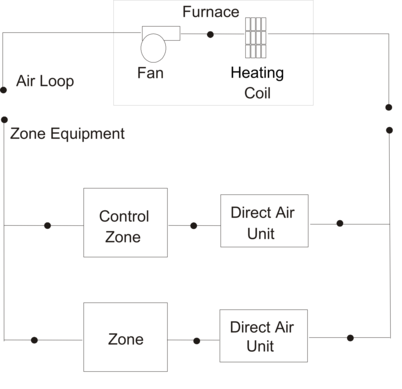
\includegraphics[width=0.9\textwidth, height=0.9\textheight, keepaspectratio=true]{media/image302.png}
\caption{Schematic of Blow Through Furnace Model \protect \label{fig:schematic-of-blow-through-furnace-model}}
\end{figure}

Links to the fan and heating coil specifications are provided in the furnace input data syntax. In addition the control zone name and the furnace design operating conditions are specified by the furnace inputs.

\subsubsection{Inputs}\label{inputs-5-033}

\paragraph{Field: Name}\label{field-name-6-025}

This alpha field contains the identifying name for the furnace.

\paragraph{Field: Availability Schedule Name}\label{field-availability-schedule-name-5-004}

This alpha field contains the schedule name which contains information on the availability of the furnace to operate. A schedule value equal to 0 denotes that the furnace must be off for that time period. A value greater than 0 denotes that the furnace is available to operate during that time period. This schedule may be used to completely disable the unitary system as required. If this field is left blank, the schedule has a value of 1 for all time periods.

\paragraph{Field: Furnace Inlet Node Name}\label{field-furnace-inlet-node-name}

This alpha field contains the furnace inlet node name.

\paragraph{Field: Furnace Outlet Node Name}\label{field-furnace-outlet-node-name}

This alpha field contains the furnace outlet node name.

\textbf{\emph{Field: Supply Air Fan Operating Mode Schedule Name}}

This alpha field specifies the name of the supply air fan operating mode schedule. The supply air fan operating mode may vary during the simulation based on time-of-day or with a change of season. Schedule values of 0 denote that the furnace supply air fan and the heating coil cycle on and off together to meet the heating load (a.k.a. AUTO fan). Schedule values other than 0 denote that the supply fan runs continuously while the heating coil cycles to meet the load.

\paragraph{Field: Maximum Supply Air Temperature}\label{field-maximum-supply-air-temperature-3}

This numeric field contains the design operating furnace air outlet temperature in degrees C when the furnace is heating. If this input field is left blank, the default value is 80 C.

\paragraph{Field: Heating Supply Air Flow Rate}\label{field-heating-supply-air-flow-rate-4-000}

This numeric field contains the design volumetric flow rate of the furnace in cubic meters per second. This volumetric flow rate should match the flow rate specified for the furnace fan.

\paragraph{Field: Controlling Zone or Thermostat Location}\label{field-controlling-zone-or-thermostat-location-5}

This alpha field contains the identifying zone name where the thermostat controlling the furnace is located.

\paragraph{Field: Supply Fan Object Type}\label{field-supply-fan-object-type-3}

This alpha field contains the identifying type of supply air fan specified for the furnace. Fan type must be \textbf{\hyperref[fanonoff]{Fan:OnOff}} or \textbf{\hyperref[fanconstantvolume]{Fan:ConstantVolume}}. \hyperref[fanconstantvolume]{Fan:ConstantVolume} is used when the Supply Air Fan Operating Mode Schedule values are never 0 and the fan operates continuously. \hyperref[fanonoff]{Fan:OnOff} is used when the fan cycles on and off with the cooling or heating coil (i.e.~Supply Air Fan Operating Mode Schedule values are at times 0).

\paragraph{Field: Supply Fan Name}\label{field-supply-fan-name-3}

This alpha field contains the identifying name given to the furnace fan.

\paragraph{Field: Fan Placement}\label{field-fan-placement-4}

This alpha field has two choices: \textbf{BlowThrough} or \textbf{DrawThrough}. The first choice stands for ``blow through fan''. This means that the unit consists of a fan followed by the heating coil. The fan ``blows through'' the heating coil. The second choice stands for ``draw through fan''. This means that the unit consists of the heating coil followed by a fan. The fan ``draws air through'' the heating coil. If this field is left blank, the default is blow through.

\paragraph{Field: Heating Coil Object Type}\label{field-heating-coil-object-type-5}

This alpha field contains the identifying type of heating coil specified in the furnace. The hot water and steam heating coils require specifying plant loop, branches, and connectors objects to support the heating coils, and are placed on the demand side of the plantloop. The hot water flow modulation through the heating coil does not require additional controller or \hyperref[controllerwatercoil]{Controller:WaterCoil} object. The parent object (Unitary Heat Only Furnace) itself provides the ``controller'' function of modulating water flow. Heating coil type must be:

\begin{itemize}
\item
  \hyperref[coilheatingelectric]{Coil:Heating:Electric}
\item
  \hyperref[coilheatinggas-000]{Coil:Heating:Fuel}
\item
  \hyperref[coilheatingwater]{Coil:Heating:Water}
\item
  \hyperref[coilheatingsteam]{Coil:Heating:Steam}
\end{itemize}

\paragraph{Field: Heating Coil Name}\label{field-heating-coil-name-5}

This alpha field contains the identifying name given to the furnace heating coil.

As shown in the example below, correct specification of the furnace requires specification of the following objects in addition to the furnace object:

1)~~~fan (\hyperref[fanonoff]{Fan:OnOff} or \hyperref[fanconstantvolume]{Fan:ConstantVolume})

2)~~~heating coil (\hyperref[coilheatinggas-000]{Coil:Heating:Fuel} or \hyperref[coilheatingelectric]{Coil:Heating:Electric})

3)~~~direct air unit (\hyperref[airterminalsingleductconstantvolumenoreheat]{AirTerminal:SingleDuct:ConstantVolume:NoReheat}) for each zone served by the furnace

Note: the furnace's fan and heating coil must be connected in the air loop according to the configuration shown above (Figure~\ref{fig:schematic-of-blow-through-furnace-model}) when a blow through fan configuration is specified. If a draw through fan is used, the fan is located down stream of the heating coil. In addition, the volumetric air flow rate specified in the direct air unit for the controlling zone should properly reflect the fractional volumetric air flow rate specified in the furnace object.

\begin{lstlisting}

AirLoopHVAC:Unitary:Furnace:HeatOnly,
      Gas Furnace 1,        !- Name
      FanAndCoilAvailSched, !- Availability Schedule Name
      Air Loop Inlet Node,  !- Furnace Air Inlet Node Name
      Air Loop Outlet Node, !- Furnace Air Outlet Node Name
      CycFanSchedule,       !- Supply Air Fan Operating Mode Schedule Name
      80,                   !- Maximum Supply Air Temperature {C}
      1.3,                  !- Heating Supply Air Flow Rate {m3/s}
      East Zone,            !- Controlling Zone or Thermostat Location
      Fan:OnOff,            !- Supply Fan Object Type
      Supply Fan 1,         !- Supply Fan Fame
      BlowThrough,          !- Fan Placement
      Coil:Heating:Fuel,     !- Heating Coil Object Type
      Furnace Coil;         !- Heating Coil Name


    Coil:Heating:Fuel,
      Furnace Coil,          !- Coil Name
      FanAndCoilAvailSched,  !- Availability Schedule Name
      NaturalGas,            !- Fuel Type
      0.8,                   !- Gas Burner Efficiency of the Coil
      20000,                 !- Nominal Capacity of the Coil {W}
      Heating Coil Air Inlet Node,  !- Coil_Air_Inlet_Node
      Air Loop Outlet Node,         !- Coil_Air_Outlet_Node
      ,                      !- Coil_Temp_Setpoint_Node
      100,                   !- Parasitic Electric Load {W}
      PLFCurveforGasFurnace, !- Part load fraction correlation (function of part load ratio)
      10;                    !- Parasitic Gas Load {W}


  Curve:Cubic,
      PLFCurveforGasFurnace, !- Name
      0.8,  !- Coefficient1 Constant
      0.2,  !- Coefficient2 x
      0.0,  !- Coefficient3 x**2
      0.0,  !- Coefficient4 x**3
      0,  !- Minimum Value of x
      1;  !- Maximum Value of x


    Fan:OnOff,
      Supply Fan 1,          !- Fan Name
      FanAndCoilAvailSched,  !- Availability Schedule Name
      0.7,    !- Fan Total Efficiency
      600.0,  !- Delta Pressure {Pa}
      1.3,    !- Max Flow Rate {m3/s}
      0.9,    !- Motor Efficiency
      1.0,    !- Motor In Airstream Fraction
      Air Loop Inlet Node,          !- Fan_Inlet_Node
      Heating Coil Air Inlet Node;  !- Fan_Outlet_Node


    AirTerminal:SingleDuct:ConstantVolume:NoReheat,
      Zone1DirectAir,              !- Name
      ,                            !- Availability Schedule Name
      Zone 1 Terminal Inlet Node,  !- Air Inlet Node Name
      Zone 1 Supply Node,          !- Air Outlet Node Name
      0.47;                        !- Maximum air flow rate {m3/s}

    AirTerminal:SingleDuct:ConstantVolume:NoReheat,
      Zone2DirectAir,              !- Name
      ,                            !- Availability Schedule Name
      Zone 2 Terminal Inlet Node,  !- Air Inlet Node Name
      Zone 2 Supply Node,          !- Air Outlet Node Name
      0.36;                        !- Maximum air flow rate {m3/s}

    AirTerminal:SingleDuct:ConstantVolume:NoReheat,
      Zone3DirectAir,              !- Name
      ,                            !- Availability Schedule Name
      Zone 3 Terminal Inlet Node,  !- Air Inlet Node Name
      Zone 3 Supply Node,          !- Air Outlet Node Name
      0.47;                        !- Maximum air flow rate {m3/s}
\end{lstlisting}

Example of Heat-Only Furnace Specification

\subsubsection{Outputs}\label{outputs-4-018}

\begin{itemize}
\tightlist
\item
  HVAC,Average,Unitary System Fan Part Load Ratio {[]}
\end{itemize}

\paragraph{Unitary System Fan Part Load Ratio {[]}}\label{unitary-system-fan-part-load-ratio-5}

This output variable is the ratio of actual air mass flow rate through the furnace to the furnace's design air mass flow rate (i.e., design volumetric flow rate converted to dry air mass flow rate). For continuous fan operation mode, this variable is always 1.0 when the furnace is available (based on the availability schedule). For cycling fan/cycling coil operation mode, the actual air mass flow rate is calculated based on the ratio of the sensible heating load to the furnace heating capacity. For the cycling fan mode, the runtime fraction for the furnace fan may be different from the fan part-load ratio reported here due the part-load performance of the furnace's heating coil (delay at start-up to reach steady-state heating output). In general, runtime fractions are reported by individual components where appropriate (e.g., Fan:OnOff).

\subsection{AirLoopHVAC:UnitaryHeatOnly}\label{airloophvacunitaryheatonly}

The AirLoopHVAC:UnitaryHeatOnly is identical to the \hyperref[airloophvacunitaryfurnaceheatonly]{AirLoopHVAC:Unitary:Furnace:HeatOnly} model. The heat-only unitary system is a ``virtual'' component that consists of a fan component (OnOff or ConstantVolume) and a Gas or Electric heating coil component. The blow through unitary system configuraion is shown in the Figure below.

\begin{figure}[hbtp] % fig 121
\centering
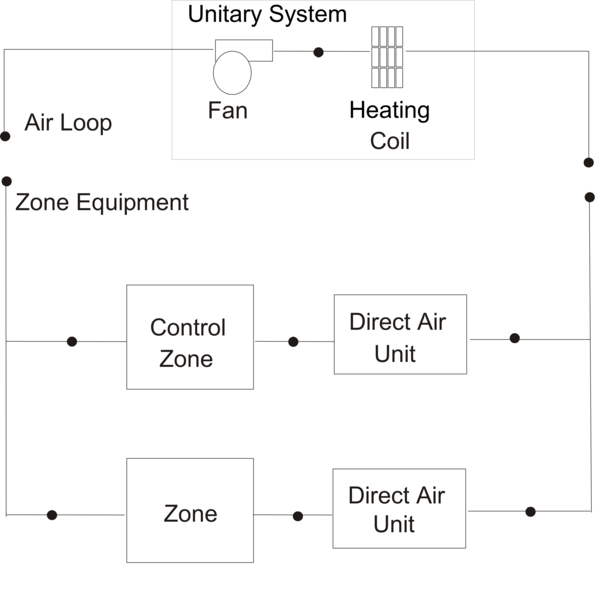
\includegraphics[width=0.9\textwidth, height=0.9\textheight, keepaspectratio=true]{media/image303.png}
\caption{Schematic of Blow Through Heat-Only Unitary System \protect \label{fig:schematic-of-blow-through-heat-only-unitary}}
\end{figure}

Links to the fan and heating coil specifications are provided in the unitary system input data syntax. In addition, the control zone name and the unitary system design operating conditions are specified by the unitary system syntax.

\subsubsection{Inputs}\label{inputs-6-030}

\paragraph{Field: Name}\label{field-name-7-023}

This alpha field contains the identifying name for the unitary system.

\paragraph{Field: Availability Schedule Name}\label{field-availability-schedule-name-6-004}

This alpha field contains the schedule name which contains information on the availability of the unitary system to operate. A schedule value equal to 0 denotes that the unitary system must be off for that time period. A value greater than 0 denotes that the unitary system is available to operate during that time period. This schedule may be used to completely disable the unitary system as required. If this field is left blank, the schedule has a value of 1 for all time periods.

\paragraph{Field: Unitary System Air Inlet Node Name}\label{field-unitary-system-air-inlet-node-name-2}

This alpha field contains the unitary system inlet node name.

\paragraph{Field: Unitary System Air Outlet Node Name}\label{field-unitary-system-air-outlet-node-name-2}

This alpha field contains the unitary system outlet node name.

\textbf{\emph{Field: Supply Air Fan Operating Mode Schedule Name}}

This alpha field specifies the name of the supply air fan operating mode schedule. The supply air fan operating mode may vary during the simulation based on time-of-day or with a change of season. Schedule values of 0 denote that the furnace supply air fan and the heating coil cycle on and off together to meet the heating load (a.k.a. AUTO fan). Schedule values other than 0 denote that the supply fan runs continuously while the heating coil cycles to meet the load.

\paragraph{Field: Maximum Supply Air Temperature}\label{field-maximum-supply-air-temperature-4}

This numeric field contains the design~ air outlet temperature in degrees C when the unitary system is heating. If this input field is left blank, the default value is 80 C.

\paragraph{Field: Heating Supply Air Flow Rate}\label{field-heating-supply-air-flow-rate-5-000}

This numeric field contains the design volumetric flow rate of the unitary system in cubic meters per second. This volumetric flow rate should match the flow rate specified for the unitary system fan.

\paragraph{Field: Controlling Zone or Thermostat Location}\label{field-controlling-zone-or-thermostat-location-6}

This alpha field contains the identifying zone name where the thermostat controlling the unitary system is located.

\paragraph{Field: Supply Fan Object Type}\label{field-supply-fan-object-type-4}

This alpha field contains the identifying type of supply air fan specified for the unitary system. Fan type must be \textbf{\hyperref[fanonoff]{Fan:OnOff}} or \textbf{\hyperref[fanconstantvolume]{Fan:ConstantVolume}}. \hyperref[fanconstantvolume]{Fan:ConstantVolume} is used when the Supply Air Fan Operating Mode Schedule values are never 0 and the fan operates continuously. \hyperref[fanonoff]{Fan:OnOff} is used when the fan cycles on and off with the cooling or heating coil (i.e.~Supply Air Fan Operating Mode Schedule values are at times 0).

\paragraph{Field: Supply Fan Name}\label{field-supply-fan-name-4}

This alpha field contains the identifying name given to the unitary system fan.

\paragraph{Field: Fan Placement}\label{field-fan-placement-5}

This alpha field has two choices: \textbf{BlowThrough} or \textbf{DrawThrough}. The first choice stands for ``blow through fan''. This means that the unit consists of a fan followed by the heating coil. The fan ``blows through'' the heating coil. The second choice stands for ``draw through fan''. This means that the unit consists of the heating coil followed by a fan. The fan ``draws air through'' the heating coil. If this field is left blank, the default is blow through.

\paragraph{Field: Heating Coil Object Type}\label{field-heating-coil-object-type-6}

This alpha field contains the identifying type of heating coil specified in the unitary system. The hot water and steam heating coils require specifying plant loop, branches, and connectors objects to support the heating coils, and are placed on the demand side of the plantloop. The hot water flow modulation through the heating coil does not require additional controller or \hyperref[controllerwatercoil]{Controller:WaterCoil} object. The parent object (Unitary Heat Only) itself provides the ``controller'' function of modulating water flow. Heating coil type must be:

\begin{itemize}
\item
  \hyperref[coilheatingelectric]{Coil:Heating:Electric}
\item
  \hyperref[coilheatinggas-000]{Coil:Heating:Fuel}
\item
  \hyperref[coilheatingwater]{Coil:Heating:Water}
\item
  \hyperref[coilheatingsteam]{Coil:Heating:Steam}
\end{itemize}

\paragraph{Field: Heating Coil Name}\label{field-heating-coil-name-6}

This alpha field contains the identifying name given to the unitary system heating coil.

As shown in the example below, correct specification of the heat-only unitary system requires specification of the following objects in addition to the unitary system object:

1)~~~fan (\hyperref[fanonoff]{Fan:OnOff} or \hyperref[fanconstantvolume]{Fan:ConstantVolume})

2)~~~heating coil (\hyperref[coilheatinggas-000]{Coil:Heating:Fuel} or \hyperref[coilheatingelectric]{Coil:Heating:Electric})

3)~~~direct air unit (\hyperref[airterminalsingleductconstantvolumenoreheat]{AirTerminal:SingleDuct:ConstantVolume:NoReheat}) for each zone served by the furnace

Note: the unitary system's fan and heating coil must be connected in the air loop according to the configuration shown above (Figure~\ref{fig:schematic-of-blow-through-heat-only-unitary}) when a blow through fan configuration is specified. If a draw through fan is used, the fan is located down stream of the heating coil. In addition, the volumetric air flow rate specified in the direct air unit for the controlling zone should properly reflect the fractional volumetric air flow rate specified in the unitary system object.

\begin{lstlisting}

AirLoopHVAC:UnitaryHeatOnly,
      Gas Unitary System 1, !- Name
      FanAndCoilAvailSched, !- Availability Schedule Name
      Air Loop Inlet Node,  !- Unitary System Air Inlet Node Name
      Air Loop Outlet Node, !- Unitary System Air Outlet Node Name
      CycFanSchedule,       !- Supply Air Fan Operating Mode Schedule Name
      80,                   !- Maximum Supply Air Temperature {C}
      1.3,                  !- Heating Supply Air Flow Rate {m3/s}
      East Zone,            !- Controlling Zone or Thermostat Location
      Fan:OnOff,            !- Supply Fan Object Type
      Supply Fan 1,         !- Supply Fan Name
      BlowThrough,          !- Fan Placement
      Coil:Heating:Fuel,     !- Heating Coil Object Type
      Unitary System Heating Coil; !- Heating Coil Name


    Coil:Heating:Fuel,
      Unitary System Heating Coil, !- Coil Name
      FanAndCoilAvailSched,        !- Availability Schedule Name
      NaturalGas,                 !- Fuel Type
      0.8,                         !- Gas Burner Efficiency of the Coil
      20000,                       !- Nominal Capacity of the Coil {W}
      Heating Coil Air Inlet Node, !- Coil_Air_Inlet_Node
      Air Loop Outlet Node,        !- Coil_Air_Outlet_Node
      ,                            !- Coil_Temp_Setpoint_Node
      100,                         !- Parasitic Electric Load {W}
      PLFCurveforUnitarySystem,    !- Part load fraction correlation (function of part load ratio)
      10;                          !- Parasitic Gas Load {W}


  Curve:Cubic,
      PLFCurveforUnitarySystem,  !- Name
      0.8,  !- Coefficient1 Constant
      0.2,  !- Coefficient2 x
      0.0,  !- Coefficient3 x**2
      0.0,  !- Coefficient4 x**3
      0,  !- Minimum Value of x
      1;  !- Maximum Value of x


  Fan:OnOff,
      Supply Fan 1,          !- Fan Name
      FanAndCoilAvailSched,  !- Availability Schedule Name
      0.7,    !- Fan Total Efficiency
      600.0,  !- Delta Pressure {Pa}
      1.3,    !- Max Flow Rate {m3/s}
      0.9,    !- Motor Efficiency
      1.0,    !- Motor In Airstream Fraction
      Air Loop Inlet Node,          !- Fan_Inlet_Node
      Heating Coil Air Inlet Node;  !- Fan_Outlet_Node


    AirTerminal:SingleDuct:ConstantVolume:NoReheat,
      Zone1DirectAir,              !- Name
      ,                            !- Availability Schedule Name
      Zone 1 Terminal Inlet Node,  !- Air Inlet Node Name
      Zone 1 Supply Node,          !- Air Outlet Node Name
      0.47;                        !- Maximum air flow rate {m3/s}

    AirTerminal:SingleDuct:ConstantVolume:NoReheat,
      Zone2DirectAir,              !- Name
      ,                            !- Availability Schedule Name
      Zone 2 Terminal Inlet Node,  !- Air Inlet Node Name
      Zone 2 Supply Node,          !- Air Outlet Node Name
      0.36;                        !- Maximum air flow rate {m3/s}

    AirTerminal:SingleDuct:ConstantVolume:NoReheat,
      Zone3DirectAir,              !- Name
      ,                            !- Availability Schedule Name
      Zone 3 Terminal Inlet Node,  !- Air Inlet Node Name
      Zone 3 Supply Node,          !- Air Outlet Node Name
      0.47;                        !- Maximum air flow rate {m3/s}
\end{lstlisting}

Example of Heat-Only Unitary System Specification

\subsubsection{Outputs}\label{outputs-5-011}

\begin{itemize}
\tightlist
\item
  HVAC,Average,Unitary System Fan Part Load Ratio {[]}
\end{itemize}

\paragraph{Unitary System Fan Part Load Ratio {[]}}\label{unitary-system-fan-part-load-ratio-6}

This output variable is the ratio of actual air mass flow rate through the unitary system to the unitary system's design air mass flow rate (i.e., design volumetric flow rate converted to dry air mass flow rate). For continuous fan operation mode, this variable is always 1.0 when the unitary system is available (based on the availability schedule). For cycling fan/cycling coil operation mode, the actual air mass flow rate is calculated based on the ratio of the sensible heating load to the unitary system heating capacity. For the cycling fan mode, the runtime fraction for the unitary system fan may be different from the fan part-load ratio reported here due the part-load performance of the unitary system's heating coil (delay at start-up to reach steady-state heating output). In general, runtime fractions are reported by individual components where appropriate (e.g., Fan:OnOff).

\subsection{AirLoopHVAC:UnitaryHeatPump:WaterToAir}\label{airloophvacunitaryheatpumpwatertoair}

The unitary water-to-air heat pump is similar to the unitary air-to-air heat pump except water is used on the source side. Links to the fan, WaterToAirHeatPump cooling coil, WaterToAirHeatPump heating coil, and supplementary heating coil specifications are provided in the heat pump's input data syntax. The heat pump switches between cooling and heating depending on the zone's demand. The load side (air) of the unitary water-to-air heat pump consists of an On/Off fan component, a WaterToAirHeatPump cooling coil component, a WaterToAirHeatPump heating coil component, and a Gas, Electric, Steam, or Hot Water supplemental heating coil component. The source side (water) of the heat pump is connected to a condenser loop with a heat exchanger (ground heat exchanger or other type) or a plant loop with a heating source such as a boiler and a cooling source such as a chiller or cooling tower. The diagram below shows the setup and connection of the heat pump for the source side and load side for a ground heat exchanger configuration. Note that on the load side, the WaterToAirHeatPump cooling coil must always be placed before the WaterToAirHeatPump heating coil.

There are three type of WaterToAirHeatPump coil models available:

\begin{itemize}
\item
  \hyperref[coilcoolingwatertoairheatpumpparameterestimation]{Coil:Cooling:WaterToAirHeatPump:ParameterEstimation}
\item
  \hyperref[coilheatingwatertoairheatpumpparameterestimation]{Coil:Heating:WaterToAirHeatPump:ParameterEstimation}
\item
  \hyperref[coilcoolingwatertoairheatpumpequationfit]{Coil:Cooling:WaterToAirHeatPump:EquationFit}
\item
  \hyperref[coilheatingwatertoairheatpumpequationfit]{Coil:Heating:WaterToAirHeatPump:EquationFit}
\item
  \hyperref[coilcoolingwater]{Coil:Cooling:Water}toAirHeat\hyperref[pumpvariablespeed]{Pump:VariableSpeed}EquationFit
\item
  \hyperref[coilheatingwater]{Coil:Heating:Water}toAirHeat\hyperref[pumpvariablespeed]{Pump:VariableSpeed}EquationFit
\end{itemize}

\begin{figure}[hbtp] % fig 122
\centering
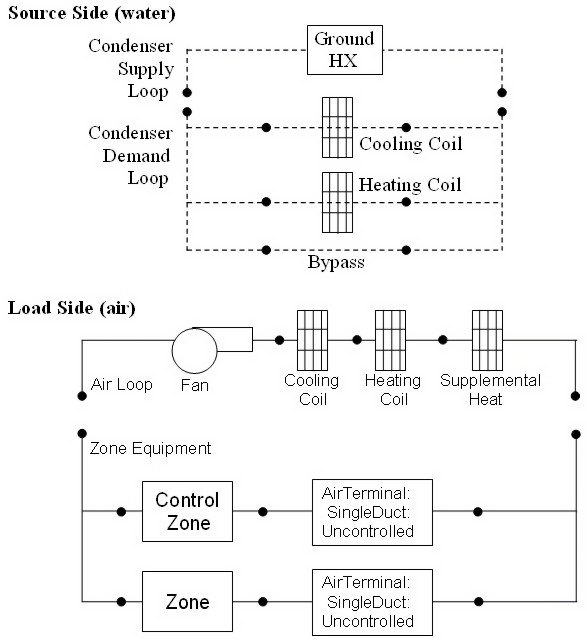
\includegraphics[width=0.9\textwidth, height=0.9\textheight, keepaspectratio=true]{media/image304.png}
\caption{Water to Air Heat Pump Schematic for a BlowThrough Configuration with Ground Heat Exchanger \protect \label{fig:water-to-air-heat-pump-schematic-for-a}}
\end{figure}

In addition, the control zone name and the system design operating conditions are specified by the heat pump inputs.

\subsubsection{Inputs}\label{inputs-7-029}

\paragraph{Field: Name}\label{field-name-8-023}

This alpha field contains the identifying name for the unitary system heat pump.

\paragraph{Field: Availability Schedule Name}\label{field-availability-schedule-name-7-004}

This alpha field contains the schedule name (ref. Schedule objects) that contains information on the availability of the heat pump to operate. A schedule value greater than 0 (usually 1 is used) indicates that the unit can be on during the time period. A value less than or equal to 0 (usually 0 is used) denotes that the unit must be off for the time period. If this field is left blank, the schedule has a value of 1 for all time periods.

\paragraph{Field: Air Inlet Node Name}\label{field-air-inlet-node-name-2-002}

This alpha field contains the name of the HVAC system node from which the heat pump draws its inlet air.

\paragraph{Field: Air Outlet Node Name}\label{field-air-outlet-node-name-2-002}

This alpha field contains the name of the HVAC system node to which the heat pump sends its outlet air.

\paragraph{Field: Supply Air Flow Rate}\label{field-supply-air-flow-rate}

This numeric field contains the design volumetric flow rate through the heat pump in cubic meters per second. This volume flow rate is only used when the cooling and heating coil object type is Coil:*:WaterToAirHeatPump:ParameterEstimation. Although a value greater than 0 is required (input cannot be blank or 0), this input is not used for the EquationFit model. Instead, the supply air flow rate is determined by the input in the corresponding Coil:*:WaterToAirHeatPump:EquationFit objects.

\paragraph{Field: Controlling Zone or Thermostat Location}\label{field-controlling-zone-or-thermostat-location-7}

This alpha field contains the identifying zone name where the thermostat controlling the heat pump is located.

\paragraph{Field: Supply Air Fan Object Type}\label{field-supply-air-fan-object-type-2}

This alpha field contains the identifying type of supply air fan specified in the heat pump. Fan type must be \hyperref[fanonoff]{Fan:OnOff}.

\paragraph{Field: Supply Air Fan Name}\label{field-supply-air-fan-name-2}

This alpha field contains the identifying name given to the heat pump supply air fan, and should match the name specified in the corresponding fan object.

\paragraph{Field: Heating Coil Object Type}\label{field-heating-coil-object-type-7}

This alpha field contains the identifying type of heating coil specified in the heat pump. Heating coil types are:

\begin{itemize}
\item
  \hyperref[coilheatingwatertoairheatpumpparameterestimation]{Coil:Heating:WaterToAirHeatPump:ParameterEstimation}
\item
  \hyperref[coilheatingwatertoairheatpumpequationfit]{Coil:Heating:WaterToAirHeatPump:EquationFit}
\item
  \hyperref[coilheatingwatertoairheatpumpvariablespeedequationfit]{Coil:Heating:WaterToAirHeat\hyperref[pumpvariablespeed]{Pump:VariableSpeed}EquationFit}
\end{itemize}

\paragraph{Field: Heating Coil Name}\label{field-heating-coil-name-7}

This alpha field contains the identifying name given to the WaterToAirHeatPump heating coil, and should match the name specified in the corresponding WaterToAirHeatPump heating coil object.

\paragraph{Field: Heating Convergence}\label{field-heating-convergence}

This numeric value allows the user to determine how close the air side has to be controlled. Lower the value of convergence better the control of air side conditions and less the zone temperature fluctuations. However in a poorly designed system, a lower convergence might result in warning errors which are caused due to the iteration limit for run time fraction calculation is limited to 20.

\paragraph{Field: Cooling Coil Object Type}\label{field-cooling-coil-object-type-5}

This alpha field contains the identifying type of cooling coil specified in the heat pump. Cooling coil types are:

\begin{itemize}
\item
  \hyperref[coilcoolingwatertoairheatpumpparameterestimation]{Coil:Cooling:WaterToAirHeatPump:ParameterEstimation}
\item
  \hyperref[coilcoolingwatertoairheatpumpequationfit]{Coil:Cooling:WaterToAirHeatPump:EquationFit}
\item
  \hyperref[coilcoolingwatertoairheatpumpvariablespeedequationfit]{Coil:Cooling:WaterToAirHeat\hyperref[pumpvariablespeed]{Pump:VariableSpeed}EquationFit}
\end{itemize}

\paragraph{Field: Cooling Coil Name}\label{field-cooling-coil-name-5}

This alpha field contains the identifying name given to the WaterToAirHeatPump cooling coil, and should match the name specified in the corresponding WaterToAirHeatPump cooling coil object.

\paragraph{Field: Cooling Convergence}\label{field-cooling-convergence}

This numeric value allows the user to determine how close the air side has to be controlled. Lower the value of convergence better the control of air side conditions and less the zone temperature fluctuations. However in a poorly designed system, a lower convergence might result in warning errors which are caused due to the iteration limit for run time fraction calculation is limited to 20.

\paragraph{Field: Maximum Cycling Rate}\label{field-maximum-cycling-rate-1-000}

This numeric field contains the maximum on-off cycling rate for the compressor, which occurs at 50\% run time fraction. Suggested values are shown below (Henderson et al. 1999):

\begin{figure}[htbp]
\centering
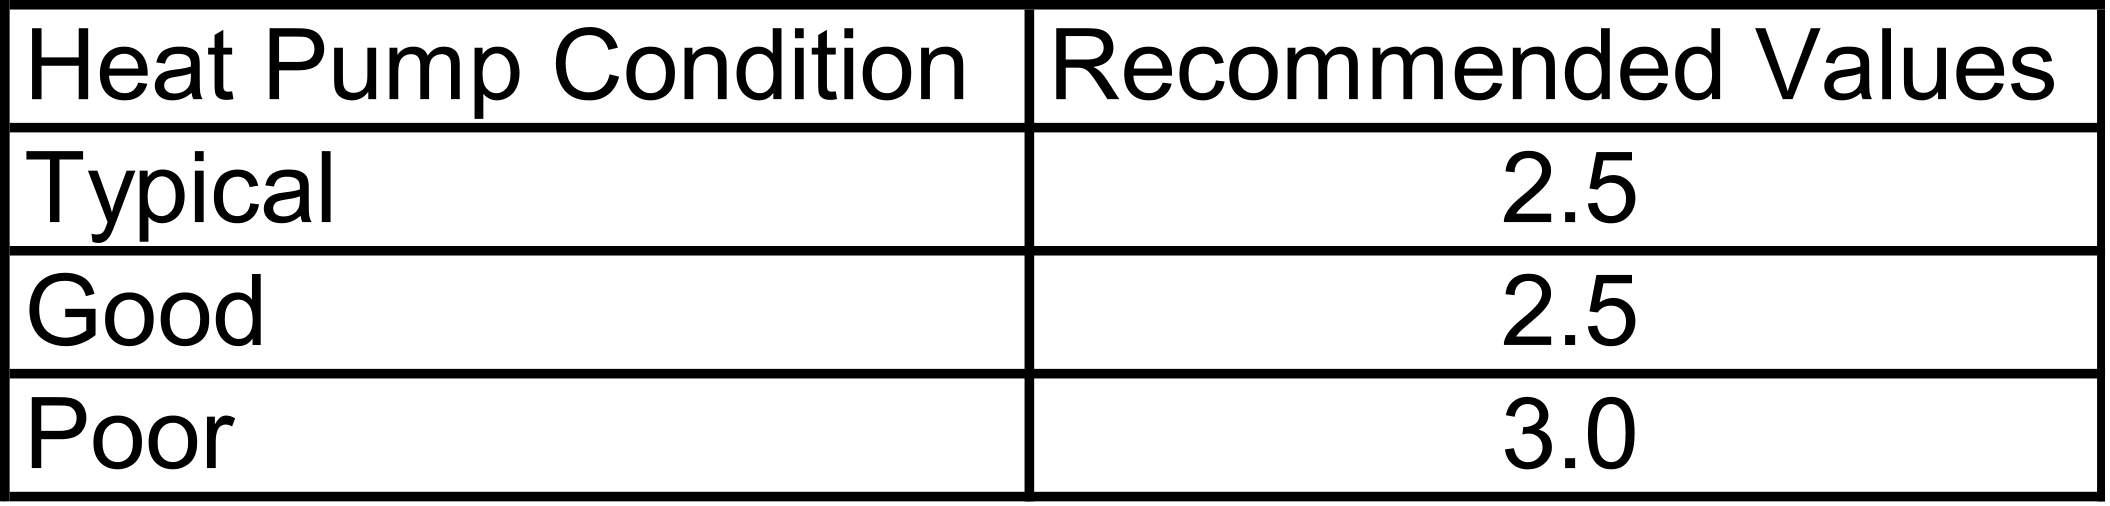
\includegraphics{media/image305.png}
\caption{}
\end{figure}

\paragraph{Field: Heat Pump Time Constant}\label{field-heat-pump-time-constant-1}

This numeric field contains the time constant for the cooling coil's capacity to reach steady state after startup. Suggested values are shown below (Henderson et al. 1999):

\begin{figure}[htbp]
\centering
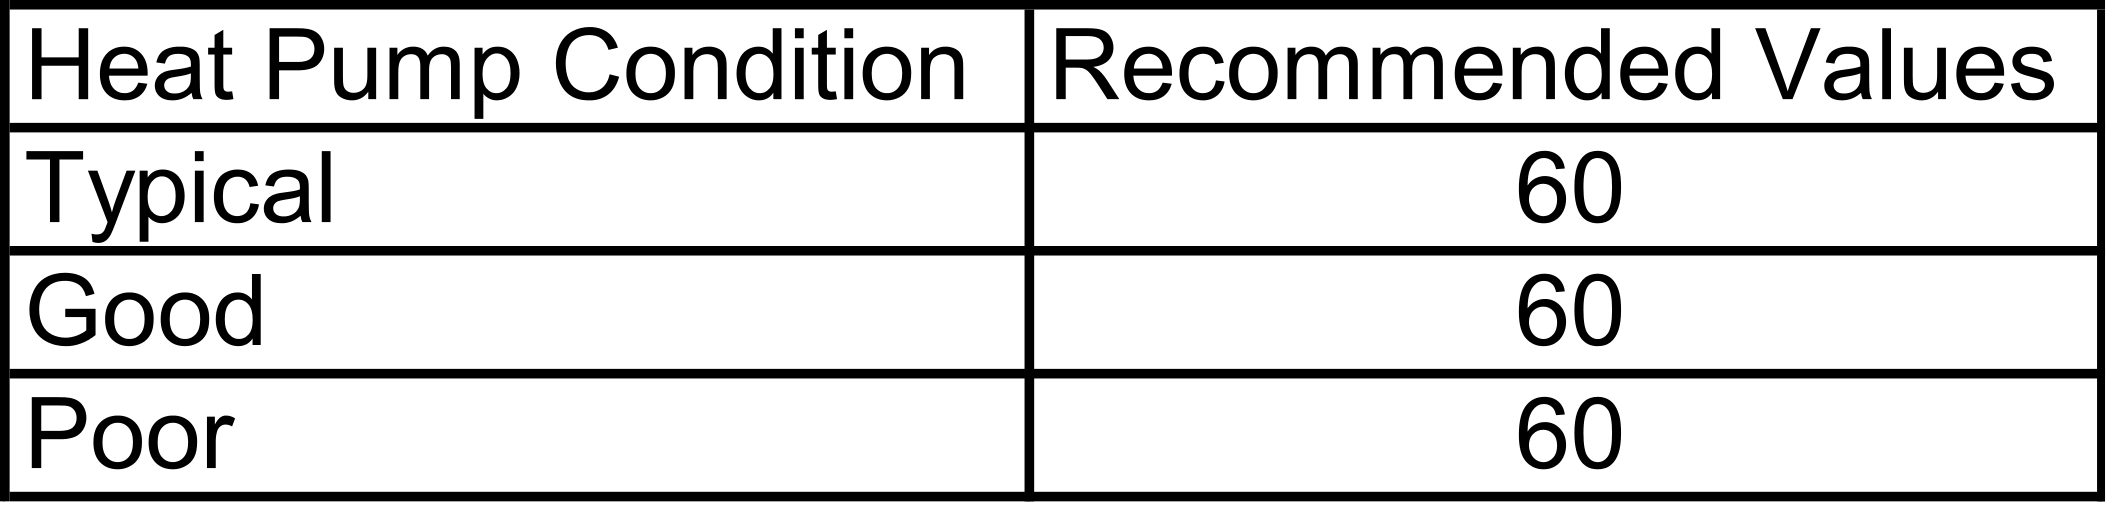
\includegraphics{media/image306.png}
\caption{}
\end{figure}

\paragraph{Field: Fraction of On-Cycle Power Use}\label{field-fraction-of-on-cycle-power-use-1}

This numeric field contains the fraction of on-cycle power use to adjust the part load fraction based on the off-cycle power consumption due to crankcase heaters, controls, fans, and etc. Suggested value values are below (Henderson et al. 1999):

\begin{figure}[htbp]
\centering
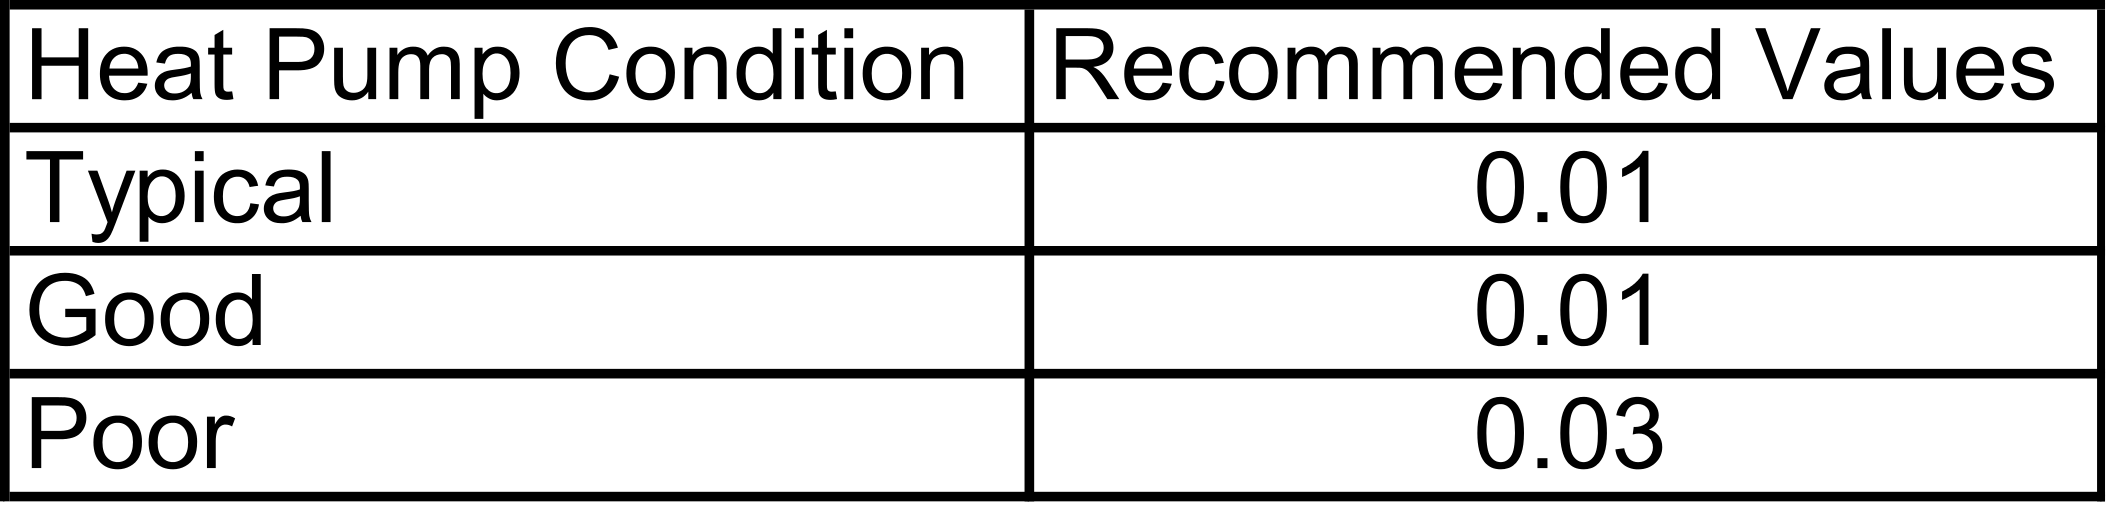
\includegraphics{media/image307.png}
\caption{}
\end{figure}

\paragraph{Field: Heat Pump Fan Delay Time}\label{field-heat-pump-fan-delay-time-1}

This numeric field contains the time delay for the heat pump supply air fan to shut off after the compressor cycles off in seconds. This value can be obtained from the manufacturer or the heat pump catalog. Enter a value of zero when the heat pump's fan operating mode is continuous. Suggested value is 60 seconds.

\paragraph{Field: Supplemental Heating Coil Object Type}\label{field-supplemental-heating-coil-object-type-3}

This is the object type of the supplemental heating coil. The hot water and steam heating coils require specifying plant loop, branches, and connectors objects to support the heating coils, and are placed on the demand side of the plantloop. The hot water flow modulation through the supplemental heating coil does not require additional controller or \hyperref[controllerwatercoil]{Controller:WaterCoil} object. The parent object (AirLoop Unitary Water to Air Heat Pump) itself provides the ``controller'' function of modulating water flow. The valid choices are:

\begin{itemize}
\item
  \hyperref[coilheatingelectric]{Coil:Heating:Electric}
\item
  \hyperref[coilheatinggas-000]{Coil:Heating:Fuel}
\item
  \hyperref[coilheatingwater]{Coil:Heating:Water}
\item
  \hyperref[coilheatingsteam]{Coil:Heating:Steam}
\end{itemize}

\paragraph{Field: Supplemental Heating Coil Name}\label{field-supplemental-heating-coil-name-3}

This alpha field contains the identifying name given to the supplemental heating coil, and should match the name specified in the corresponding supplemental heating coil object.

\paragraph{Field: Maximum Supply Air Temperature from Supplemental Heater}\label{field-maximum-supply-air-temperature-from-supplemental-heater-2}

This numeric field defines the maximum allowed supply air temperature exiting the heat pump supplemental heating coil in degrees Celsius.

\paragraph{Field: Maximum Outdoor Dry-Bulb Temperature for Supplemental Heater Operation}\label{field-maximum-outdoor-dry-bulb-temperature-for-supplemental-heater-operation-3}

This numeric field defines the outdoor air dry-bulb temperature in degrees Celsius above which the heat pump supplemental heating coil is disabled. The temperature for this input field must be less than or equal to 21°C. If this input field is left blank, the default value is 21°C.

\paragraph{Field: Outdoor Dry-Bulb Temperature Sensor Node Name}\label{field-outdoor-dry-bulb-temperature-sensor-node-name-1}

This alpha field specifies the name of the outdoor node which controls the operation of the supplemental heating coil. If this field is left blank, the outdoor temperature is based solely on the weather data. If this field is not blank, the node name specified must also be listed in an \hyperref[outdoorairnode]{OutdoorAir:Node} object where the height of the node is taken into consideration when calculating outdoor temperature from the weather data. Alternately, the node name must be specified in an \hyperref[outdoorairnodelist]{OutdoorAir:NodeList} object where the outdoor temperature is taken directly from the weather data.

\paragraph{Field: Fan Placement}\label{field-fan-placement-6}

This alpha field has two choices: \textbf{BlowThrough} or \textbf{DrawThrough}. The first choice represents a blow through system where the supply air fan is before the WaterToAirHeatPump cooling/heating coil and the supplementary heating coil. The second choice represents a draw through system where the supply fan is between the WaterToAirHeatPump cooling/heating coil and the supplementary heating coil. If this input field is left blank, the default is blow through.

\paragraph{Field: Supply Air Fan Operating Mode Schedule Name}\label{field-supply-air-fan-operating-mode-schedule-name-2}

This alpha field specifies the name of the supply air fan operating mode schedule. The supply air fan operating mode may vary during the simulation based on time-of-day or with a change of season. Schedule values of 0 denote that the supply air fan and the heating/cooling coil cycle on and off together to meet the heating or cooling load (a.k.a. AUTO fan). Schedule values other than 0 denote that the supply air fan runs continuously while the heating or cooling coil cycles to meet the load. If this field is left blank, the model assumes the supply air fan cycles with the heating or cooling coil throughout the simulation period.

As shown in the example below, correct specification of the water-to-air heat pump requires specification of the following objects in addition to the AirLoopHVAC:UnitaryHeatPump:WaterToAir object:

\begin{itemize}
\item
  On/Off fan
\item
  WaterToAirHeatPump cooling coil
\item
  WaterToAirHeatPump heating coil
\item
  Supplementary heating coil
\item
  Direct air unit for each zone served by the heat pump
\item
  Condenser demand branches
\end{itemize}

It should be noted that the volumetric air flow rate specified in the direct air unit for the controlling zone should properly reflect the fractional volumetric air flow rate specified in the heat pump object.

\paragraph{Field: Dehumidification Control Type}\label{field-dehumidification-control-type-4-000}

This alpha input field contains the type of dehumidification control. The following options are valid for this field:

\textbf{None} - meet sensible load only, no active dehumidification control

\textbf{CoolReheat} - cool beyond the dry-bulb temperature set point as required to meet the high humidity setpoint. The excess cooling beyond the cooling set point temperature is offset by the supplemental heating coil.

The default is \textbf{None}. For \textbf{CoolReheat} dehumidification control modes, the maximum humidity setpoint is required. This must be set using a \textbf{\hyperref[zonecontrolhumidistat]{ZoneControl:Humidistat}} object. When extra dehumidification is required, the system may not be able to meet the humidity setpoint if its full capacity is not adequate. Supplemental heating coil (supplemental heating coil type and name) is a required input in WaterToAir HeatPumps. When dehumidification control is active the heating and the reheat load due to extra dehumidification are met with supplemetal heating coil. The supplemental heating coil capacity must be adequate enough to meet the heating coil load and offset the excess cooling load due to~ extra dehumidification. The dehumidification control type CoolReheat works only with \hyperref[coilcoolingwatertoairheatpumpequationfit]{Coil:Cooling:WaterToAirHeatPump:EquationFit} cooling coil type.

\paragraph{Field: Heat Pump Coil Water Flow Mode}\label{field-heat-pump-coil-water-flow-mode-000}

This field specifies the way in which water flow through the heat pump coils will be modeled.~ This field is only used when WatertoAirHeatPump:EquationFit coils are used. There are three options:

\begin{itemize}
\item
  Cycling
\item
  Constant
\item
  CyclingOnDemand
\end{itemize}

\textbf{Cycling} varies water flow through the coil based on the heat pump Part Load Ratio.~ This control method is appropriate for modeling heat pumps that are outfitted with a soleniod valve which allows water to flow through the coil only when the compressor is active. This is the default for EnergyPlus V8 and later.

\textbf{Constant} provides a constant water flow regardless of heat pump operation.~ Remember that EnergyPlus has two coils (a heating coil and a cooling coil) to approximate the operation of one coil that can operate in either heating mode or cooling mode.~ Therefore, when the water flow mode is constant, there will be full flow through either the heating coil or the cooling coil, but not both at the same time.

\textbf{ConstantOnDemand} provides full flow through the coil whenever there is a load.~ When there is no load, there is zero flow through the coil.~ This control strategy represents the way EnergyPlus modeled heat pump water flow prior to Version 8.

Following is an example of IDF usage:

\begin{lstlisting}

AirLoopHVAC:UnitaryHeatPump:WaterToAir,
      DXAC Heat Pump 1,        !- Name
      FanAndCoilAvailSched,    !- Availability Schedule Name
      Mixed Air Node,          !- Air Inlet Node Name
      Air Loop Outlet Node,    !- Air Outlet Node Name
      2,                       !- Supply Air Flow Fate {m3/s}
      East Zone,               !- Controlling Zone or Thermostat Location
      Fan:OnOff,        !- Supply Air Fan Object Type
      Supply Fan 1,            !- Supply Air Fan Name
      Coil:Heating:WaterToAirHeatPump:ParameterEstimation,  !- Heating Coil Object Type
      Heat Pump Heating Mode,  !- Heating Coil Name
      0.001,                   !- Heating Convergence
      Coil:Cooling:WaterToAirHeatPump:ParameterEstimation,  !- Cooling Coil Object Type
      Heat Pump Cooling Mode,  !- Cooling Coil Name
      0.001,                   !- Cooling Convergence
      2.5, !- Maximum Cycling Rate {cycles/hr}
      60, !- Heat Pump Time Constant {s}
      0.01, !- Fraction of On-Cycle Power Use
      60,    !- Heat Pump Fan Delay Time {s}
      Coil:Heating:Fuel,        !- Supplemental Heating Coil Object Type
      Heat Pump DX Supp Heating Coil 1,  !- Supplemental Heating Coil Name
      50,                      !- Maximum Supply Air Temperature from Supplemental Heater {C}
      21,                      !- Maximum Outdoor Dry-Bulb Temperature for Supplemental Heater Operation {C}
      Outside Air Inlet Node, !- Outdoor Dry-Bulb Temperature Sensor Node Name
      BlowThrough,             !- Fan Placement
      CyclingFanSch,           !- Supply Air Fan Operating Mode Schedule Name
      CoolReheat;              !- Dehumidification Control Type


  Schedule:Compact,
      CyclingFanSch,           !- Name
      Fraction,                !- Schedule Type Limits Name
      Through: 12/31,          !- Field 1
      For: AllDays,            !- Field 2
      Until: 24:00,            !- Field 3
      0.0;                     !- Field 4




    Coil:Cooling:WaterToAirHeatPump:ParameterEstimation,
      Heat Pump Cooling Mode,  !- Name
      Scroll,                !- Compressor Type
      R22,                   !- Refrigerant Type
      0.0015,                  !- Design Source Side Flow Rate {m3/s}
      38000,  !- Nominal Cooling Coil Capacity {W)
      0,            !- Nominal Time for Condensate Removal to Begin {s}
      0,      !- Ratio of Initial Moisture Evaporation Rate and Steady State Latent Capacity
      3000000,                 !- High Pressure CutOff {Pa}
      0,                       !- Low Pressure CutOff {Pa}
      Water to Air Heat Pump Source Side1 Inlet Node,  !- Water Inlet Node Name
      Water to Air Heat Pump Source Side1 Outlet Node,  !- Water Outlet Node Name
      Cooling Coil Air Inlet Node,  !- Air Inlet Node Name
      Heating Coil Air Inlet Node,  !- Air Outlet Node Name
      3.78019E+03,!-Parameter 1 {W/K}
      2.80303E+03,!- Parameter 2 {W/K}
     7.93591E-01,!- Parameter 3 {C}
      1.91029E+03,!- Parameter 4 {W}
      2.66127E+00,!- Parameter 5
      1.06009E-02,!- Parameter 6
      1.65103E+00,!- Parameter 7
      9.73887E-03,!- Parameter 8
      1.04563E+03;!- Parameter 9




   Coil:Heating:WaterToAirHeatPump:ParameterEstimation,
      Heat Pump HEATING Mode,  !- Name
      Scroll,                !- Compressor Type
      R22,                   !- Refrigerant Type
      0.0015,                  !- Design Source Side Flow Rate {m3/s}
      38000,                   !- Nominal Heating Coil Capacity {W}
      3000000,                 !- High Pressure CutOff
      0,                       !- Low Pressure CutOff {Pa}
      Water to Air Heat Pump Source Side2 Inlet Node,  !- Water Inlet Node Name
      Water to Air Heat Pump Source Side2 Outlet Node,  !- Water Outlet Node Name
      Heating Coil Air Inlet Node,  !- Air Inlet Node Name
      SuppHeating Coil Air Inlet Node,  !- Air Outlet Node Name
      3.91379E+03,  !-Parameter 1 {W/K}
      5.94753E-01,  !- Parameter 2 {C}
      2.49945E+03,  !- Parameter 3 {W}
      8.68734E-01,  !- Parameter 4
      7.23595E-03,  !- Parameter 5
      3.69126E+00,  !- Parameter 6
      1.75701E-05,  !- Parameter 7
      3.65348E+03;  !-Parameter 8




    Coil:Heating:Fuel,
      Heat Pump DX Supp Heating Coil 1,  !- Name
      FanAndCoilAvailSched,    !- Availability Schedule Name
      NaturalGas,              !- Fuel Type
      0.8,                     !- Gas Burner Efficiency
      32000,                   !- Nominal Capacity {W}
      SuppHeating Coil Air Inlet Node,  !- Air Inlet Node Name
      Air Loop Outlet Node;    !- Air Outlet Node Name




    BRANCH,
      Gshp Cooling Condenser Branch,  !- Name
      , !- Pressure Drop Curve Name
      Coil:Cooling:WaterToAirHeatPump:ParameterEstimation,  !- Component 1 Object Type
      Heat Pump Cooling Mode,  !- Component 1 Name
      Water to Air Heat Pump Source Side1 Inlet Node, !- Component 1 Inlet Node Name
      Water to Air Heat Pump Source Side1 Outlet Node; !- Component 1 Outlet Node Name


    BRANCH,
      Gshp Heating Condenser Branch,  !- Name
      , !- Pressure Drop Curve Name
      Coil:Heating:WaterToAirHeatPump:ParameterEstimation,  !- Component 1 Object Type
      Heat Pump Heating Mode,  !- Component 1 Name
      Water to Air Heat Pump Source Side2 Inlet Node,  !- Component 1 Inlet Node Name
      Water to Air Heat Pump Source Side2 Outlet Node;  !- Component 1 Outlet Node Name




    Fan:OnOff,
      Supply Fan 1,          !- Name
      FanAndCoilAvailSched,  !- Availability Schedule Name
      0.7,                   !- FanTotal Efficiency
      300.0,                 !– Pressure Rise {Pa}
      2.0,                   !- Maximum Flow Rate {m3/s}
      0.9,                   !- Motor Efficiency
      1.0,                   !- Motor In Airstream Fraction
      Mixed Air Node,        !- Air Inlet_Node Name
      Cooling Coil Air Inlet Node;  !- Air Outlet Node Name


    AirTerminal:SingleDuct:ConstantVolume:NoReheat,
      Zone1DirectAir,              !- Name
      ,                            !- Availability Schedule Name
      Zone 1 Terminal Inlet Node,  !- Air Inlet Node Name
      Zone 1 Supply Node,          !- Air Outlet Node Name
      0.7;                         !- Maximum air flow rate {m3/s}

    AirTerminal:SingleDuct:ConstantVolume:NoReheat,
      Zone2DirectAir,              !- Name
      ,                            !- Availability Schedule Name
      Zone 2 Terminal Inlet Node,  !- Air Inlet Node Name
      Zone 2 Supply Node,          !- Air Outlet Node Name
      0.6;                         !- Maximum air flow rate {m3/s}

    AirTerminal:SingleDuct:ConstantVolume:NoReheat,
      Zone3DirectAir,              !- Name
      ,                            !- Availability Schedule Name
      Zone 3 Terminal Inlet Node,  !- Air Inlet Node Name
      Zone 3 Supply Node,          !- Air Outlet Node Name
      0.7;                         !- Maximum air flow rate {m3/s}
\end{lstlisting}

\subsubsection{Outputs}\label{outputs-6-011}

Energy use reporting for the water-to-air heat pump is documented under the heat pump coil object types:

\begin{itemize}
\item
  Coil:Cooling:WaterToAirHeatPump:ParameterEstimation
\item
  Coil:Heating:WaterToAirHeatPump:ParameterEstimation
\item
  Coil:Cooling:WaterToAirHeatPump:EquationFit
\item
  Coil:Heating:WaterToAirHeatPump:EquationFit
\end{itemize}

The heat pump \emph{demand} as well as the compressor and fan part-load ratios may be obtained with the output variables shown below.

\begin{itemize}
\item
  HVAC,Average, Unitary System Requested Sensible Cooling Rate {[}W{]}
\item
  HVAC,Average, Unitary System Requested Latent Cooling Rate {[}W{]}
\item
  HVAC,Average, Unitary System Requested Heating Rate {[}W{]}
\item
  HVAC,Average, Unitary System Compressor Part Load Ratio {[]}
\item
  HVAC,Average, Unitary System Fan Part Load Ratio
\item
  HVAC,Average, Unitary System Dehumidification Induced Heating Demand Rate {[}W{]}
\end{itemize}

\paragraph{Unitary System Requested Sensible Cooling Rate {[}W{]}}\label{unitary-system-requested-sensible-cooling-rate-w-1}

This output variable is the sensible cooling requested from the zone thermostat in watts. This value is calculated using the unitary heat pump outlet air and zone conditions, the specific heat of the zone air, and the supply air mass flow rate entering/leaving the system. This value is calculated for each HVAC system timestep being simulated, and the results are averaged for the timestep being reported.

\paragraph{Unitary System Requested Latent Cooling Rate {[}W{]}}\label{unitary-system-requested-latent-cooling-rate-w-1}

This output variable is the latent cooling requested from the zone humidistat in watts. This value is calculated using the unitary heat pump outlet air and zone conditions, the heat of vaporization of water at the current zone conditions, and the supply air mass flow rate entering/leaving the system. This value is calculated for each HVAC system timestep being simulated, and the results are averaged for the timestep being reported.

\paragraph{Unitary System Requested Heating Rate {[}W{]}}\label{unitary-system-requested-heating-rate-w-1}

This output variable is the sensible heating requested from the zone thermostat in watts. This value is calculated using the unitary heat pump outlet air and zone conditions, the specific heat of the zone air, and the supply air mass flow rate entering/leaving the system. This value is calculated for each HVAC system timestep being simulated, and the results are averaged for the timestep being reported.

\paragraph{Unitary System Compressor Part Load Ratio {[]}}\label{unitary-system-compressor-part-load-ratio-4}

This output variable is the ratio of actual load on the unitary system to the unitary system's steady state output.~ This ratio is based on the nominal capacity of the unit.

\paragraph{Unitary System Fan Part Load Ratio {[]}}\label{unitary-system-fan-part-load-ratio-7}

This output variable is the ratio of actual air mass flow rate through the unitary system to the unitary system's design air mass flow rate (i.e., design volumetric flow rate converted to dry air mass flow rate). For continuous fan operation mode, this variable is always 1.0 when the unitary system is available (based on the availability schedule).

\paragraph{Unitary System Dehumidification Induced Heating Demand Rate {[}W{]}}\label{unitary-system-dehumidification-induced-heating-demand-rate-w-1}

This output variable is the additional heating demand rate of the supplemental heating coil of a Water-to-Air heat pumps in Watts.~ This additional heating demand is induced when zone air overshoots the heating setpoint due to extra dehumidification requirement to meet the high humidity setpoint. This value is always positive. This value is calculated for each HVAC system timestep, and the results are averaged for the timestep being reported.

\subsection{AirLoopHVAC:UnitaryHeatCool:VAVChangeoverBypass}\label{airloophvacunitaryheatcoolvavchangeoverbypass}

The changeover-bypass variable air volume (CBVAV) unitary system is a compound object made up of other components. Each CBVAV system consists of an outdoor air mixer, direct expansion (DX) cooling coil, heating coil, and a supply air fan as shown in the figures below. Zone thermostats and terminal units are required in each zone served by this system. The terminal units are specific to this system type and are either \hyperref[airterminalsingleductvavheatandcoolreheat]{AirTerminal:SingleDuct:VAV:HeatAndCool:Reheat} or \hyperref[airterminalsingleductvavheatandcoolnoreheat]{AirTerminal:SingleDuct:VAV:HeatAndCool:NoReheat}. A zone humidistat and single zone max humidity set point manager may also be specified to help control high humidity levels. These individual components are described elsewhere in this document. The system may also be connected to an inlet node of either the \hyperref[airloophvaczonemixer]{AirLoopHVAC:ZoneMixer} or \hyperref[airloophvacreturnplenum]{AirLoopHVAC:ReturnPlenum} to more accurately model the \hyperref[airloophvacoutdoorairsystem]{AirLoopHVAC:OutdoorAirSystem}. The CBVAV unitary system object coordinates the operation of these components and is modeled as a type of air loop equipment (Ref. \hyperref[airloophvac]{AirLoopHVAC}).

\begin{figure}[hbtp] % fig 123
\centering
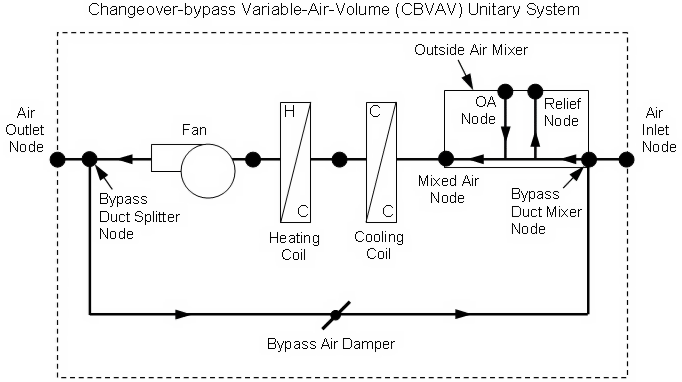
\includegraphics[width=0.9\textwidth, height=0.9\textheight, keepaspectratio=true]{media/image308.png}
\caption{Schematic of a CBVAV unitary system (draw through fan placement) \protect \label{fig:schematic-of-a-cbvav-unitary-system-draw}}
\end{figure}

\begin{figure}[hbtp] % fig 124
\centering
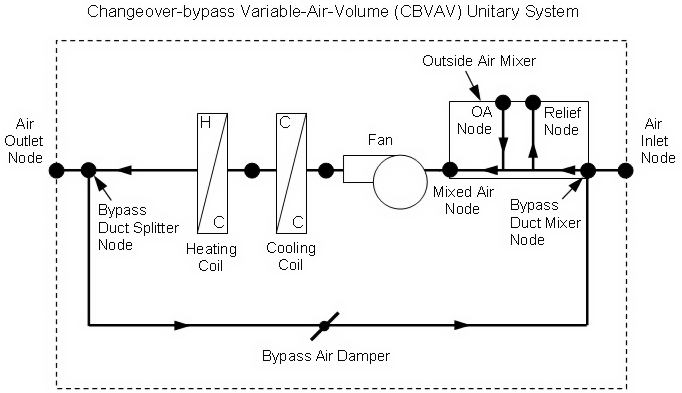
\includegraphics[width=0.9\textwidth, height=0.9\textheight, keepaspectratio=true]{media/image309.png}
\caption{Schematic of a CBVAV unitary system (blow through fan placement) \protect \label{fig:schematic-of-a-cbvav-unitary-system-blow}}
\end{figure}

\begin{figure}[hbtp]
\centering
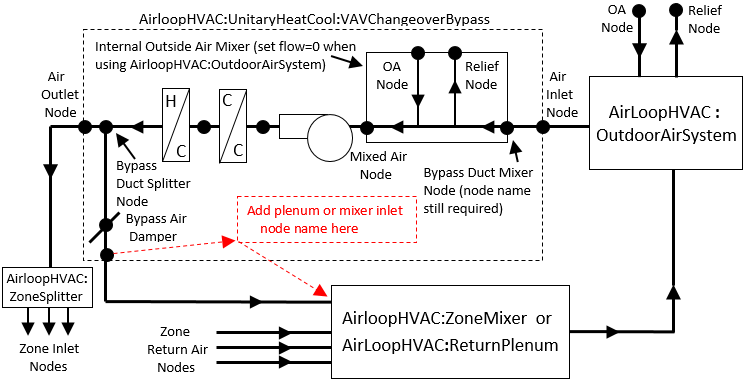
\includegraphics[width=0.9\textwidth, height=0.9\textheight, keepaspectratio=true]{media/ChangeoverBypassVAV-ReturnPlenumOrMixer.png}
\caption{Schematic of a CBVAV unitary system used with outdoor air system \protect \label{fig:schematic-of-a-cbvav-unitary-system-used-with-outdoor-air-system}}
\end{figure}

Links to the CBVAV system's supply air fan, coils, and outdoor air mixer specifications are provided in the object's input syntax. Additional inputs include system and outdoor air flow rates during heating and cooling operation, the priority control mode, and dehumidification control type. A description of each input field for the CBVAV unitary system compound object is provided below.

\subsubsection{Inputs}\label{inputs-8-027}

\paragraph{Field: Name}\label{field-name-9-020}

This alpha field defines a unique user-assigned name for an instance of a changeover-bypass VAV system. Any reference to this system by another object will use this name.

\paragraph{Field: Availability Schedule Name}\label{field-availability-schedule-name-8-004}

This alpha field defines the name of the schedule (ref: Schedule) that denotes whether the system operates during a given time period. A schedule value equal to 0 denotes that the system must be off for that time period, and a schedule value greater than 0 denotes that the system is available to operate during that time period. This schedule may be used to completely disable the system (all of its coils and the supply air fan) as required. If this field is left blank, the schedule has a value of 1 for all time periods.

\paragraph{Field: Cooling Supply Air Flow Rate}\label{field-cooling-supply-air-flow-rate-4-000}

This numeric field defines the air flow rate through the system (i.e., through the fan and heating/cooling coils) in cubic meters per second when the DX cooling coil is operating. Values must be greater than 0, or this field is autosizable.

\paragraph{Field: Heating Supply Air Flow Rate}\label{field-heating-supply-air-flow-rate-6}

This numeric field defines the air flow rate through the system (i.e., through the fan and heating/cooling coils) in cubic meters per second when the heating coil is operating. Values must be greater than 0, or this field is autosizable.

\paragraph{Field: No Load Supply Air Flow Rate}\label{field-no-load-supply-air-flow-rate-5}

This numeric field defines the air flow rate through the system (i.e., through the fan and heating/cooling coils) in cubic meters per second when neither cooling nor heating is required (i.e., the DX cooling coil and heating coil are off but the supply air fan operates). Values must be greater than or equal to zero, or this field is autosizable. This field is only used when the unitary system's supply air fan operating mode is specified as continuous fan operation (Ref. Field: Supply air fan operating mode schedule name). If the system's supply air fan operating mode is specified as continuous fan operation and this value is set to zero or the field is left blank, then the model assumes that the system air flow rate when no heating/cooling is needed is equal to the system air flow rate when the coils were last operating (for cooling operation or heating operation).

\paragraph{Field: Cooling Outdoor Air Flow Rate}\label{field-cooling-outdoor-air-flow-rate-000}

This numeric field defines the outdoor air flow rate through the system (i.e., through the Outdoor air Mixer's Outside\_Air\_Stream\_Node) in cubic meters per second when the DX cooling coil is operating. Values must be greater than or equal to 0, or this field is autosizable. Note that the Cooling Outdoor Air Flow Rate can be changed during the simulation using a multiplier schedule (Ref. Field: Outdoor air volumetric flow rate multiplier schedule name). For any simulation timestep, the Cooling Outdoor Air Flow Rate cannot exceed the system air volumetric flow rate during cooling operation.

\paragraph{Field: Heating Outdoor Air Flow Rate}\label{field-heating-outdoor-air-flow-rate-000}

This numeric field defines the outdoor air flow rate through the system (i.e., through the Outdoor air Mixer's Outside\_Air\_Stream\_Node) in cubic meters per second when the heating coil is operating. Values must be greater than or equal to 0, or this field is autosizable. Note that the Heating Outdoor Air Flow Rate can be changed during the simulation using a multiplier schedule (Ref. Field: Outdoor air volumetric flow rate multiplier schedule name). For any simulation timestep, the Heating Outdoor Air Flow Rate cannot exceed the system air volumetric flow rate during heating operation.

\paragraph{Field: No Load Outdoor Air Flow Rate When No Cooling or Heating is Needed}\label{field-no-load-outdoor-air-flow-rate-when-no-cooling-or-heating-is-needed}

This numeric field defines the outdoor air flow rate through the system (i.e., through the Outdoor air Mixer's Outside\_Air\_Stream\_Node) in cubic meters per second when neither cooling nor heating is required (i.e., the DX cooling coil and heating coil are off but the supply air fan operates). Values must be greater than or equal to 0, or this field is autosizable. Note that the no load outdoor air flow rate can be changed during the simulation using a multiplier schedule (Ref. Field: Outdoor air volumetric flow rate multiplier schedule name). For any simulation timestep, the no load outdoor air flow rate cannot exceed the no load supply air flow rate. This field is only used when the unitary system's supply air fan operating mode is specified as continuous fan operation (Ref. Field: Supply air fan operating mode schedule name). If the system's supply air fan operating mode is specified as continuous fan operation and this value is set to zero or the field is left blank, then the model assumes that the no load outdoor air flow rate is equal to the outdoor air flow rate when the coils were last operating (for cooling operation {[}i.e.~Cooling outdoor air flow rate{]} or heating operation {[}i.e.~Heating outdoor air flow rate{]}) and this field is not used.

\paragraph{Field: Outdoor Air Flow Rate Multiplier Schedule Name}\label{field-outdoor-air-flow-rate-multiplier-schedule-name}

This alpha field defines the name of a schedule (ref: Schedule) that contains multipliers for the outdoor air volume flow rates (heating, cooling, no heating/cooling). Schedule values must be from zero to 1. If this field is left blank, then the model assumes that the outdoor air multiplier is 1 for the entire simulation period.

\paragraph{Field: Air Inlet Node Name}\label{field-air-inlet-node-name-3-002}

This alpha field defines the name of the HVAC system node from which the system draws its inlet air.

\paragraph{Field: Bypass Duct Mixer Node Name}

This alpha field defines the name of the HVAC system node where the bypass air mixes with the unitary system's inlet air. This name should match the name of the Return Air Stream Node Name for the \hyperref[outdoorairmixer]{OutdoorAir:Mixer} associated with this system. This node name must be different from the system's air inlet node name.

\paragraph{Field: Bypass Duct Splitter Node Name}\label{field-bypass-duct-splitter-node-name}

This alpha field defines the name of the HVAC system node where the conditioned air is split into bypass air and supply air leaving the system (e.g., delivered to the terminal units). This splitter air node name should match the outlet node name for the last component (furthest downstream) in this unitary system. For blow through fan placement, the splitter air node is the outlet node of the heating coil. For draw through fan placement, the splitter node is the outlet node of the supply air fan.

\paragraph{Field: Air Outlet Node Name}\label{field-air-outlet-node-name-3-002}

This alpha field defines the name of the HVAC system node to which the system sends its outlet air.

\paragraph{Field: Outdoor Air Mixer Object Type}\label{field-outdoor-air-mixer-object-type}

This field specifies the type of outdoor air mixer used by this CBVAV unitary system. The outdoor air mixer component is part of the CBVAV unitary compound object. The only available outdoor air mixer type is:

\begin{itemize}
\tightlist
\item
  \hyperref[outdoorairmixer]{OutdoorAir:Mixer}
\end{itemize}

\paragraph{Field: Outdoor Air Mixer Name}\label{field-outdoor-air-mixer-name}

This alpha field defines the name of an outdoor air mixer component that composes part of the CBVAV system. The name of the outdoor air mixer's Return\_Air\_Stream\_Node should match the bypass duct mixer node name, and be different from the CBVAV system's air inlet node name. The Mixed Air Node Name of the outdoor air mixer should be the same as the CBVAV system's supply fan inlet air node (for blow through fan placement) or the system's DX cooling coil inlet node (for draw through fan placement).

\paragraph{Field: Supply Air Fan Object Type}\label{field-supply-air-fan-object-type-3}

This alpha field defines the type of fan used by this unitary system. The only valid choices are \textbf{\hyperref[fansystemmodel]{Fan:SystemModel}}, \textbf{\hyperref[fanonoff]{Fan:OnOff}}, and \textbf{\hyperref[fanconstantvolume]{Fan:ConstantVolume}}. The input requirements for these fan objects are described elsewhere in this document.

\paragraph{Field: Supply Air Fan Name}\label{field-supply-air-fan-name-3}

This alpha field defines the name of the fan component that composes part of this unitary system. Note that the fan component's maximum flow rate should be greater than or equal to the largest system air volumetric flow rate specified for this unitary system (heating, cooling, and no heating/cooling). In addition, the fan's inlet air node should be the same as the outdoor air mixer's Mixed Air Node (for blow through fan placement) or the heating coil's outlet node (for draw through fan placement). The fan outlet air node should be the same as the DX cooling coil's air inlet node (for blow through fan placement) or the system's bypass duct splitter node (for draw through fan placement).

\paragraph{Field: Supply Air Fan Placement}\label{field-supply-air-fan-placement-1}

This alpha field defines the placement of the supply air fan within this unitary system. The only valid choices are \textbf{BlowThrough} and \textbf{DrawThrough}. With blow through placement, the supply air fan is located immediately upstream of the system's cooling coil. With draw through placement, the supply air fan is located immediately downstream of the heating coil.

\paragraph{Field: Supply Air Fan Operating Mode Schedule Name}\label{field-supply-air-fan-operating-mode-schedule-name-3}

This alpha field defines the name of a schedule that specifies the supply air fan operating mode during the simulation. A schedule value of 0 denotes the fan cycles off when no cooling or heating is required, and any other value denotes that the fan runs continuously regardless of the need for heating or cooling. If this field is left blank, the model assumes continuous supply air fan operation for the entire simulation period.

\paragraph{Field: Cooling Coil Object Type}\label{field-cooling-coil-object-type-6}

This alpha field defines the type of cooling coil used by this unitary system. There are three valid choices for this field:

\begin{itemize}
\item
  \hyperref[coilcoolingdxsinglespeed]{Coil:Cooling:DX:SingleSpeed}
\item
  \hyperref[coilcoolingdxvariablespeed]{Coil:Cooling:DX:VariableSpeed}
\item
  \hyperref[coilsystemcoolingdxheatexchangerassisted]{CoilSystem:Cooling:DX:HeatExchangerAssisted}
\item
  \hyperref[coilcoolingdxtwostagewithhumiditycontrolmode]{Coil:Cooling:DX:TwoStageWithHumidityControlMode}
\end{itemize}

The input requirements for these cooling coil objects are described elsewhere in this document.

\paragraph{Field: Cooling Coil Name}\label{field-cooling-coil-name-6}

This alpha field defines the name of the cooling coil used by this unitary system, and this name should match the name specified in the corresponding cooling coil object.

\paragraph{Field: Heating Coil Object Type}\label{field-heating-coil-object-type-8}

This alpha field defines the type of heating coil used by this unitary system. The hot water and steam heating coils require specifying plant loop, branches, and connector objects to support the heating coils, and are placed on the demand side of the plantloop. The hot water flow modulation through the heating coil does not require additional controller or \hyperref[controllerwatercoil]{Controller:WaterCoil} object. The parent object (CBVAV Unitary System) itself provides the ``controller'' function of modulating water flow. The valid choices are:

\begin{itemize}
\item
  \hyperref[coilheatingelectric]{Coil:Heating:Electric}
\item
  \hyperref[coilheatinggas-000]{Coil:Heating:Fuel}
\item
  \hyperref[coilheatingdxsinglespeed]{Coil:Heating:DX:SingleSpeed}
\item
  \hyperref[coilheatingdxvariablespeed]{Coil:Heating:DX:VariableSpeed}
\item
  \hyperref[coilheatingwater]{Coil:Heating:Water}
\item
  \hyperref[coilheatingsteam]{Coil:Heating:Steam}
\end{itemize}

The input requirements for these heating coil objects are described elsewhere in this document.

\paragraph{Field: Heating Coil Name}\label{field-heating-coil-name-8}

This alpha field defines the name of the heating coil used by this unitary system, and this name should match the name specified in the corresponding heating coil object.

\paragraph{Field: Priority Control Mode}\label{field-priority-control-mode}

This choice field defines the cooling or heating priority control mode for the unitary system. Valid choices are:

\begin{itemize}
\item
  CoolingPriority
\item
  HeatingPriority
\item
  ZonePriority
\item
  LoadPriority
\end{itemize}

If CoolingPriority is selected, the system operates to meet the cooling load if any zone served by this system (air loop) requires cooling. If no zones require cooling, then the system operates in heating mode if needed. If HeatingPriority is selected, the system operates to meet the heating load if any zone requires heating. If no zones require heating, then the system operates in cooling mode if needed. If ZonePriority is selected, the system operates based on the maximum number of zones requiring either heating or cooling. If the number of zones requiring cooling is greater than the number of zones requiring heating, then the system operates in cooling mode. If the number of zones requiring heating is greater than the number of zones requiring cooling, then the system operates in heating mode. If the number of zones requiring cooling equals the number of zones requiring heating, then the largest combined load (i.e., the sum of the cooling loads for zones requiring cooling compared to the sum of the heating loads for zones that require heating) sets the cooling or heating operating mode for the system during that simulation timestep. If LoadPriority is selected, the system operates based on the largest combined load (i.e., the sum of the cooling loads for zones requiring cooling compared to the sum of the heating loads for zones that require heating). If the toal load for zones requiring cooling is greater than the toal load for zones requiring heating, then the system operates in cooling mode. Similar logic is used for heating mode selection. If the toal cooling load equals the toal heating load, then cooling or heating operation reverts to the total number of zones requiring cooling or heating (and if equal reverts to cooling mode if the cooling load is non-zero, otherwise, heating mode.

\paragraph{Field: Minimum Outlet Air Temperature During Cooling Operation}\label{field-minimum-outlet-air-temperature-during-cooling-operation}

This numeric field defines the minimum outlet air temperature leaving the system when the unit is operating to provide cooling. Values are specified in degrees Celsius and must be greater than 0. The default value is 8°C. This value must be less than or equal to the maximum outlet air temperature during heating operation.

\paragraph{Field: Maximum Outlet Air Temperature During Heating Operation}\label{field-maximum-outlet-air-temperature-during-heating-operation}

This numeric field defines the maximum outlet air temperature leaving the system when the unit is operating to provide heating. Values are specified in degrees Celsius and must be greater than 0. The default value is 50°C. This value must be greater than or equal to the minimum outlet air temperature during cooing operation.

\paragraph{Field: Dehumidification Control Type}\label{field-dehumidification-control-type-5-000}

This alpha field contains the type of dehumidification control. The following options are valid for this field:

\textbf{None} - meet sensible load only, no active dehumidification control

\textbf{Multimode} - activate enhanced dehumidification mode as needed and meet sensible load. This option is used to model DX equipment with a controllable heat exchanger assisting the DX cooling coil for improved dehumidification. It is valid only with cooling coil type = \hyperref[coilcoolingdxtwostagewithhumiditycontrolmode]{Coil:Cooling:DX:TwoStageWithHumidityControlMode}.

\textbf{CoolReheat} - cool beyond the dry-bulb temperature set point as required to meet the high humidity setpoint. It is valid only with cooling coil type = \hyperref[coilcoolingdxtwostagewithhumiditycontrolmode]{Coil:Cooling:DX:TwoStageWithHumidityControlMode}.

The default is \textbf{None}. For the other dehumidification control modes, the maximum humidity setpoint on the CBVAV system's air outlet node is used. This must be set using a \textbf{\hyperref[zonecontrolhumidistat]{ZoneControl:Humidistat}} and one of:

\begin{itemize}
\item
  \textbf{\hyperref[setpointmanagersinglezonehumiditymaximum]{SetpointManager:SingleZone:Humidity:Maximum}}
\item
  \textbf{\hyperref[setpointmanagermultizonehumiditymaximum]{SetpointManager:MultiZone:Humidity:Maximum}}
\item
  \textbf{\hyperref[setpointmanagermultizonemaximumhumidityaverage]{SetpointManager:MultiZone:MaximumHumidity:Average}}
\end{itemize}

objects. When extra dehumidification is required, the system may not be able to meet the humidity setpoint if its full capacity is not adequate.

\paragraph{Field: Plenum or Mixer Inlet Node Name}\label{field-bypass-duct-mixer-node-name}

This alpha field defines the name of the HVAC system node where the bypass air enters the zone mixer or return plenum. This node name must be different from the system's \textbf{\hyperref[field-air-outlet-node-name-3-002]{Air Outlet Node Name}} and \textbf{\hyperref[field-bypass-duct-splitter-node-name]{Bypass Duct Splitter Node Name}}. This name should match the name of the inlet node in the \hyperref[airloophvaczonemixer]{AirLoopHVAC:ZoneMixer} or \hyperref[airloophvacreturnplenum]{AirLoopHVAC:ReturnPlenum} associated with this system.

\paragraph{Field: Minimum Runtime Before Operating Mode Change}\label{minimum-runtime-before-operating-mode-change}

This numeric field defines the amount of time, in hours, the HVAC system operates before a mode change is allowed. The value entered must be greater than or equal to 0. The default value is 0.25 hours if this input is present and blank. If this field is not present the minimum runtime is 0 hours (i.e., immediate change over as needed).
\medskip

As shown in the example below, correct specification of the CBVAV unitary system requires specification of the following objects in addition to the AirLoopHVAC:UnitaryHeatCool:VAVChangeoverBypass object:

1)~~~outdoor air mixer (\hyperref[outdoorairmixer]{OutdoorAir:Mixer})

2)~~~fan (\hyperref[fansystemmodel]{Fan:SystemModel}, \hyperref[fanonoff]{Fan:OnOff}, or \hyperref[fanconstantvolume]{Fan:ConstantVolume})

3)~~~cooling coil (\hyperref[coilcoolingdxsinglespeed]{Coil:Cooling:DX:SingleSpeed}, \hyperref[coilsystemcoolingdxheatexchangerassisted]{CoilSystem:Cooling:DX:HeatExchangerAssisted}, or \hyperref[coilcoolingdxtwostagewithhumiditycontrolmode]{Coil:Cooling:DX:TwoStageWithHumidityControlMode})

4)~~~heating coil (\hyperref[coilheatinggas-000]{Coil:Heating:Fuel}, \hyperref[coilheatingelectric]{Coil:Heating:Electric}, or \hyperref[coilheatingdxsinglespeed]{Coil:Heating:DX:SingleSpeed})

5)~~~terminal unit for each zone being served by this system (\hyperref[airterminalsingleductvavheatandcoolreheat]{AirTerminal:SingleDuct:VAV:HeatAndCool:Reheat} or \hyperref[airterminalsingleductvavheatandcoolnoreheat]{AirTerminal:SingleDuct:VAV:HeatAndCool:NoReheat})

6)~~~When the Plenum or Mixer Inlet Node Name is specified, this node name must connect to either the \hyperref[airloophvaczonemixer]{AirLoopHVAC:ZoneMixer} or \hyperref[airloophvacreturnplenum]{AirLoopHVAC:ReturnPlenum} and the \hyperref[airloophvacoutdoorairsystem]{AirLoopHVAC:OutdoorAirSystem} may then be used to control the outdoor air flow rates. When using the AirloopHVAC:OutdoorAirSystem it is recommended that the Cooling, Heating and No Load Outdoor Air Flow Rate inputs are set to 0, otherwise the amount of outdoor air is increased and the coils may not autosize properly.

Note: The fan, heating coil, cooling coil, and outdoor air mixer must be connected in the air loop according to the configurations shown above (Figure~\ref{fig:schematic-of-a-cbvav-unitary-system-draw}, Figure~\ref{fig:schematic-of-a-cbvav-unitary-system-blow} or Figure~\ref{fig:schematic-of-a-cbvav-unitary-system-used-with-outdoor-air-system}).

\begin{lstlisting}

AirLoopHVAC:UnitaryHeatCool:VAVChangeoverBypass,
  GasHeat CBVAV System,  !- Name of unitary system
  FanAndCoilAvailSched,  !- Availability schedule name
  1.8,                   !- Cooling Supply Air Flow Rate {m3/s}
  1.7,                   !- Heating Supply Air Flow Rate {m3/s}
  1.6,                   !- No Load Supply Air Flow Rate {m3/s}
  0.32,                  !- Cooling Outdoor Air Flow Rate {m3/s}
  0.3,                   !- Heating Outdoor Air Flow Rate {m3/s}
  0.27,                  !- No Load Outdoor Air Flow Rate {m3/s}
  Outdoor Air Multiplier Schedule, !- Outdoor air volumetric flow rate multiplier schedule name
  Air Loop Inlet Node,     !- Air inlet node name
  Mixer Inlet Node,        !- Bypass duct mixer node name
  Heating Coil Air Outlet Node,    !- Bypass duct splitter node name
  Air Loop Outlet Node,    !- Air outlet node name
  OutdoorAir:Mixer,        !- Outdoor Air Mixer Object Type
  Outdoor air Mixer,       !- Outdoor air mixer name
  Fan:OnOff,        !- Supply air fan type
  Supply Fan 1,            !- Supply air fan name
  BlowThrough,            !- Supply air fan placement
  Fan OpMode Schedule,     !- Supply air fan operating mode schedule name
  Coil:Cooling:DX:TwoStageWithHumidityControlMode,  !- Cooling coil type
  ACDXCoil 2,              !- Cooling coil name
  Coil:Heating:Fuel,        !- Heating coil type
  Furnace Heating Coil 1,  !- Heating coil name
  CoolingPriority,        !- Priority control mode
  10.0,                    !- Minimum outlet air temperature during cooling operation {C}
  50.0,                    !- Maximum outlet air temperature during heating operation {C}
  None;                    !- Dehumidification control type

  OutdoorAir:Mixer,
      Outdoor air Mixer,       !- Name
      Mixed Air Node,          !- Mixed Air Node Name
      Outdoor air Inlet Node,  !- Outdoor Air Stream Node
      Relief Air Outlet Node,  !- Relief Air Stream Node Name
      Mixer Inlet Node;        !- Return Air Stream Node Name

  Fan:OnOff,
      Supply Fan 1,            !- Fan Name
      FanAndCoilAvailSched,    !- Availability Schedule Name
      0.7,                     !- Fan Total Efficiency
      600.0,                   !- Delta Pressure {Pa}
      1.8,                     !- Max Flow Rate {m3/s}
      0.9,                     !- Motor Efficiency
      1.0,                     !- Motor In Airstream Fraction
      Mixed Air Node,          !- Fan\_Inlet\_Node
      DX Cooling Coil Air Inlet Node;  !- Fan\_Outlet\_Node

  Coil:Cooling:DX:TwoStageWithHumidityControlMode,
      ACDXCoil 2,              !- Coil Name
      FanAndCoilAvailSched,    !- Availability Schedule
      DX Cooling Coil Air Inlet Node, !- Coil Air Inlet Node
      Heating Coil Air Inlet Node,    !- Coil Air Outlet Node
      ,                        !- Crankcase Heater Capacity {W}
      ,                        !- Maximum Outdoor Dry-bulb Temperature for Crankcase Heater Operation {C}
      2,                       !- Number of Capacity Stages
      0,                       !- Number of Enhanced Dehumidification Modes
      CoilPerformance:DX:Cooling,  !- Normal Mode Stage 1 Coil Performance Object Type
      ACDXCoil 2 Standard Mode-Stage 1,  !- Normal Mode Stage 1 Coil Performance Object Name
      CoilPerformance:DX:Cooling,  !- Normal Mode Stage 1+2 Coil Performance Object Type
      ACDXCoil 2 Standard Mode-Stage 1&2;  !- Normal Mode Stage 1+2 Coil Performance Object Name

  Coil:Heating:Fuel,
      Furnace Heating Coil 1,  !- Coil Name
      FanAndCoilAvailSched,    !- Availability Schedule Name
      NaturalGas,              !- Fuel Type
      0.8,                     !- Gas Burner Efficiency of the Coil
      35000,                   !- Nominal Capacity of the Coil {W}
      Heating Coil Air Inlet Node,  !- Coil\_Air\_Inlet\_Node
      Heating Coil Air Outlet Node; !- Coil\_Air\_Outlet\_Node

  AirTerminal:SingleDuct:VAV:HeatAndCool:Reheat,
      Zone 1 VAV System,       !- Name of System
      FanAndCoilAvailSched,    !- System Availability schedule
      Zone 1 Reheat Air Inlet Node,  !- DAMPER Air Outlet Node
      Zone 1 VAV Inlet Node,   !-UNIT Air Inlet Node
      0.583,                   !- Maximum air flow rate {m3/s}
      0.25,                    !- Zone Minimum Air Flow Fraction
      ,                        !- Control node
      Coil:Heating:Electric,   !- Reheat Component Object
      Reheat Coil Zone 1,      !- Name of Reheat Component
      0.0,                     !- Max Reheat Water Flow {m3/s}
      0.0,                     !- Min Reheat Water Flow {m3/s}
      Zone 1 Reheat Air Outlet Node,  !- UNIT Air Outlet Node
      0.001;                   !- Convergence Tolerance

  AirTerminal:SingleDuct:VAV:HeatAndCool:Reheat,
      Zone 2 VAV System,       !- Name of System
      FanAndCoilAvailSched,    !- System Availability schedule
      Zone 2 Reheat Air Inlet Node,  !- DAMPER Air Outlet Node
      Zone 2 VAV Inlet Node,   !-UNIT Air Inlet Node
      0.583,                   !- Maximum air flow rate {m3/s}
      0.25,                    !- Zone Minimum Air Flow Fraction
      ,                        !- Control node
      Coil:Heating:Electric,   !- Reheat Component Object
      Reheat Coil Zone 2,      !- Name of Reheat Component
      0.0,                     !- Max Reheat Water Flow {m3/s}
      0.0,                     !- Min Reheat Water Flow {m3/s}
      Zone 2 Reheat Air Outlet Node,  !- UNIT Air Outlet Node
      0.001;                   !- Convergence Tolerance

  AirTerminal:SingleDuct:VAV:HeatAndCool:NoReheat,
      Zone 3 VAV System,       !- Name of System
      FanAndCoilAvailSched,    !- System Availability schedule
      Zone 3 Reheat Air Outlet Node,  !- UNIT Air Outlet Node
      Zone 3 VAV Inlet Node,   !-UNIT Air Inlet Node
      0.584,                   !- Maximum air flow rate {m3/s}
      0.25;                    !- Zone Minimum Air Flow Fraction
\end{lstlisting}

\subsubsection{Outputs}\label{outputs-7-011}

\begin{itemize}
\item
  HVAC,Average,Unitary System Total Heating Rate {[}W{]}
\item
  HVAC,Sum,Unitary System Total Heating Energy {[}J{]}
\item
  HVAC,Average,Unitary System Total Cooling Rate {[}W{]}
\item
  HVAC,Sum,Unitary System Total Cooling Energy {[}J{]}
\item
  HVAC,Average,Unitary System Sensible Heating Rate {[}W{]}
\item
  HVAC,Sum,Unitary System Sensible Heating Energy {[}J{]}
\item
  HVAC,Average,Unitary System Sensible Cooling Rate {[}W{]}
\item
  HVAC,Sum,Unitary System Sensible Cooling Energy {[}J{]}
\item
  HVAC,Average,Unitary System Latent Heating Rate {[}W{]}
\item
  HVAC,Sum,Unitary System Latent Heating Energy {[}J{]}
\item
  HVAC,Average,Unitary System Latent Cooling Rate {[}W{]}
\item
  HVAC,Sum,Unitary System Latent Cooling Energy {[}J{]}
\item
  HVAC,Average,Unitary System Electric Power {[}W{]}
\item
  HVAC,Sum,Unitary System Electric Energy {[}J{]}
\item
  HVAC,Average,Unitary System Fan Part Load Ratio {[]}
\item
  HVAC,Average,Unitary System Compressor Part Load Ratio {[]}
\item
  HVAC,Average,Unitary System Bypass Air Mass Flow Rate {[}kg/s{]}
\item
  HVAC,Average,Unitary System Air Outlet Setpoint Temperature {[}C{]}
\item
  HVAC,Average,Unitary System Operating Mode Index {[]}
\end{itemize}

\paragraph{Unitary System Total Heating Rate {[}W{]}}\label{unitary-system-total-heating-rate-w-2}

This output field is the total (enthalpy) heat addition rate of the CBVAV system in Watts. This value is calculated using the enthalpy difference of the outlet air and inlet air streams, and the supply air mass flow rate entering/leaving the system. This value is calculated for each HVAC system timestep being simulated, and the results (enthalpy addition only) are averaged for the timestep being reported.

\paragraph{Unitary System Total Heating Energy {[}J{]}}\label{unitary-system-total-heating-energy-j}

This output field is the total (enthalpy) heat addition of the CBVAV system in Joules over the timestep being reported. This value is calculated using the enthalpy difference of the outlet air and inlet air streams, the supply air mass flow rate entering/leaving the system, and the HVAC simulation timestep. This value is calculated for each HVAC system timestep being simulated, and the results (enthalpy addition only) are summed for the timestep being reported.

\paragraph{Unitary System Total Cooling Rate {[}W{]}}\label{unitary-system-total-cooling-rate-w-2}

This output field is the total (enthalpy) heat extraction rate of the CBVAV system in Watts. This value is calculated using the enthalpy difference of the outlet air and inlet air streams, and the supply air mass flow rate entering/leaving the system. This value is calculated for each HVAC system timestep being simulated, and the results (enthalpy extraction only) are averaged for the timestep being reported.

\paragraph{Unitary System Total Cooling Energy {[}J{]}}\label{unitary-system-total-cooling-energy-j}

This output field is the total (enthalpy) heat extraction of the CBVAV system in Joules over the timestep being reported. This value is calculated using the enthalpy difference of the outlet air and inlet air streams, the supply air mass flow rate entering/leaving the system, and the HVAC simulation timestep. This value is calculated for each HVAC system timestep being simulated, and the results (enthalpy extraction only) are summed for the timestep being reported.

\paragraph{Unitary System Sensible Heating Rate {[}W{]}}\label{unitary-system-sensible-heating-rate-w-2}

This output field is the sensible heat addition rate of the CBVAV system in Watts. This value is calculated using the enthalpy difference of the outlet air and inlet air streams at a constant humidity ratio, and the supply air mass flow rate entering/leaving the system. This value is calculated for each HVAC system timestep being simulated, and the results (heating only) are averaged for the timestep being reported.

\paragraph{Unitary System Sensible Heating Energy {[}J{]}}\label{unitary-system-sensible-heating-energy-j}

This output field is the sensible heat addition of the CBVAV system in Joules over the timestep being reported. This value is calculated using the enthalpy difference of the outlet air and inlet air streams at a constant humidity ratio, the supply air mass flow rate entering/leaving the system, and the HVAC simulation timestep. This value is calculated for each HVAC system timestep being simulated, and the results (heating only) are summed for the timestep being reported.

\paragraph{Unitary System Sensible Cooling Rate {[}W{]}}\label{unitary-system-sensible-cooling-rate-w-2}

This output field reports the moist air sensible heat extraction rate of the CBVAV system in Watts. This value is calculated using the enthalpy difference of the outlet air and inlet air streams at a constant humidity ratio, and the supply air mass flow rate entering/leaving the system. This value is calculated for each HVAC system timestep being simulated, and the results (cooling only) are averaged for the timestep being reported.

\paragraph{Unitary System Sensible Cooling Energy {[}J{]}}\label{unitary-system-sensible-cooling-energy-j}

This output field reports the moist air sensible heat extraction of the CBVAV system in Joules over the timestep being reported. This value is calculated using the enthalpy difference of the outlet air and inlet air streams at a constant humidity ratio, the supply air mass flow rate entering/leaving the system, and the HVAC simulation timestep. This value is calculated for each HVAC system timestep being simulated, and the results (cooling only) are summed for the timestep being reported.

\paragraph{Unitary System Latent Heating Rate {[}W{]}}\label{unitary-system-latent-heating-rate-w-2}

This output field is the latent heat addition (humidification) rate of the CBVAV system in Watts. This value is calculated as the difference between the total energy rate and the sensible energy rate provided by the system. This value is calculated for each HVAC system timestep being simulated, and the results (latent heat addition only) are averaged for the timestep being reported.

\paragraph{Unitary System Latent Heating Energy {[}J{]}}\label{unitary-system-latent-heating-energy-j}

This output field is the latent heat addition (humidification) of the CBVAV system in Joules over the timestep being reported. This value is calculated as the difference between the total energy and the sensible energy delivered by the system. This value is calculated for each HVAC system timestep being simulated, and the results (latent heat addition only) are summed for the timestep being reported.

\paragraph{Unitary System Latent Cooling Rate {[}W{]}}\label{unitary-system-latent-cooling-rate-w-2}

This output field is the latent heat extraction (dehumidification) rate of the CBVAV system in Watts. This value is calculated as the difference between the total energy rate and the sensible energy rate provided by the system. This value is calculated for each HVAC system timestep being simulated, and the results (latent heat extraction only) are averaged for the timestep being reported.

\paragraph{Unitary System Latent Cooling Energy {[}J{]}}\label{unitary-system-latent-cooling-energy-j}

This output field is the latent heat extraction (dehumidification) of the CBVAV system in Joules over the timestep being reported. This value is calculated as the difference between the total energy and the sensible energy delivered by the system. This value is calculated for each HVAC system timestep being simulated, and the results (latent heat extraction only) are summed for the timestep being reported.

\paragraph{Unitary System Electric Power {[}W{]}}\label{unitary-system-electric-power-w-2}

This output field is the electricity consumption rate of the CBVAV system in Watts. The consumption includes electricity used by the DX compressor (including crankcase heater), fans (indoor supply air fan and the condenser fans associated with the DX coil{[}s{]}), and the heating coil (if electric). This value is calculated for each HVAC system timestep being simulated, and the results are averaged for the timestep being reported.

\paragraph{Unitary System Electric Energy {[}J{]}}\label{unitary-system-electric-energy-j-2}

This output field is the electricity consumption of the CBVAV system in Joules for the time period being reported. The consumption includes electricity used by the DX compressor (including crankcase heater), fans (indoor supply air fan and the condenser fans associated with the DX coil{[}s{]}), and the heating coil (if electric). This value is calculated for each HVAC system timestep being simulated, and the results are summed for the timestep being reported.

\paragraph{Unitary System Fan Part Load Ratio {[]}}\label{unitary-system-fan-part-load-ratio-8}

This output field is the part-load ratio of the supply air fan, which will be either zero or 1 for each simulation timestep. For this system, the fan will operate continuously for the simulation timestep if the system is available (ref. Field: Availability schedule name) and there is a cooling or heating load to be met (i.e., fan part-load ratio will equal 1). When the system is available but there is no cooling or heating load to be met, the fan will either be off for the entire timestep or on for the entire timestep depending on the supply air fan operating mode schedule (ref. Field: Supply Air Fan Operating Mode Schedule Name). This value is set for each HVAC system timestep being simulated, and the results are averaged for the timestep being reported.

\paragraph{Unitary System Compressor Part Load Ratio {[]}}\label{unitary-system-compressor-part-load-ratio-5}

This output field is the part-load ratio of the compressor used by the DX coils (cooling and heating). The compressor part-load ratio is defined as the total coil load divided by the coil steady-state capacity (steady-state capacity of first stage for multi-mode coils). This value is calculated for each HVAC system timestep being simulated, and the results are averaged for the timestep being reported.

\paragraph{Unitary System Bypass Air Mass Flow Rate {[}kg/s{]}}\label{unitary-system-bypass-air-mass-flow-rate-kgs}

This output field is the mass flow rate of air, in kg/s, being bypassed from the supply air path and blended with the air entering the CBVAV system. This value is calculated for each HVAC system timestep being simulated, and the results are averaged for the timestep being reported.

\paragraph{Unitary System Air Outlet Setpoint Temperature {[}C{]}}\label{unitary-system-air-outlet-setpoint-temperature-c}

This output field is the dry-bulb set point temperature in degrees Celsius. This set point temperature is calculated by the model based on the zone cooling/heating loads calculated by EnergyPlus, and the priority control mode and the dehumidification control type specified for this unitary system. The CBVAV system attempts to achieve the outlet air set point temperature to the extent possible.

\paragraph{Unitary System Operating Mode Index {[]}}\label{unitary-system-operating-mode-index}

This output field is the current operating mode, either cooling, heating or no cooling or heating.  A value of 0 represents no cooling or heating is required, a value of 1 represents cooling and a value of 2 represents heating. These specific values can be seen using the detailed time step reporting frequency. If longer reporting frequencies are used (e.g., timestep, hourly, etc.) then this output is averaged over the reporting interval and the result is dependent on the value selected for \hyperref[minimum-runtime-before-operating-mode-change]{Minimum Runtime Before Operating Mode Change}.
